\documentclass[
  a4paper,
  abstract=true,
  twoside,
  listof=totoc,
  numbers=noenddot,
  bibliography=totoc,
  BCOR1.5cm,
  headsepline,
  DIV12,
  appendixprefix,
  final
] {scrreprt}

% You should select either american or british instead of english here:
\usepackage[american]{babel}
\usepackage{lmodern}
%\usepackage{fontspec}
\usepackage{afterpage}
\usepackage{tabularx}
\usepackage{mwe}
\usepackage{booktabs}
\usepackage{adjustbox}
\usepackage{subcaption}
\usepackage[pdftex,
citebordercolor={0.75 0.75 1},
filebordercolor={0.75 0.75 1},
linkbordercolor={0.75 0.75 1},
pagebordercolor={0.75 0.75 1},
urlbordercolor={0.75 0.75 1},
pdfborder={0.75 0.75 1},plainpages=false,pdfpagelabels=true]{hyperref}
\hypersetup{
  pdftitle={Privacy-preserving Smart Metering Using DC-Nets},
  pdfauthor={Gregor Garten},
  pdfkeywords={foo, bar},
}
\usepackage[acronym,nomain,toc]{glossaries}

\usepackage[backend=biber,style=alphabetic,alldates=long]{biblatex}

\usepackage{varioref}           % nice refs
\usepackage{csquotes}
\usepackage{graphicx}           % graphics
\usepackage{caption}            % manipulate fugures
\usepackage{subcaption}         % allow for subfigures
\usepackage{listings}           % nice source code listings
\usepackage{xcolor}
\usepackage{booktabs}           % nice tables
\usepackage{microtype}          % better looking text borders
\usepackage{siunitx}            % unified way of setting values with units
\usepackage{array}
\usepackage{fancybox}           % provide nice boxes
\usepackage{fancyvrb}           % algorithm-boxes
\usepackage{pdfpages}
\usepackage{hyphenat}
\usepackage{todonotes}
\usepackage{xspace}
\usepackage{setspace}

% use this one last
% (redefines some macros for compatibility with KOMAScript)
\usepackage{scrhack}

\addbibresource{own.bib}
 
\definecolor{mygreen}{rgb}{0,0.6,0}
\definecolor{mygray}{rgb}{0.5,0.5,0.5}
\definecolor{mymauve}{rgb}{0.58,0,0.82}
 
% Biblatex Style
\setcounter{secnumdepth}{3}     % limit enumeration depth
\setcounter{tocdepth}{1}        % limit TOC depth

% Listing Style

\lstset{ %
  frame=shadowbox,
  rulesepcolor=\color{blue},
  backgroundcolor=\color{white},   % choose the background color; you must add \usepackage{color} or \usepackage{xcolor}
%  basicstyle=\footnotesize,        % the size of the fonts that are used for the code
  breakatwhitespace=false,         % sets if automatic breaks should only happen at whitespace
  breaklines=true,                 % sets automatic line breaking
  captionpos=b,                    % sets the caption-position to bottom
  commentstyle=\color{mygreen},    % comment style
  deletekeywords={...},            % if you want to delete keywords from the given language
  escapeinside={\%*}{*)},          % if you want to add LaTeX within your code
  extendedchars=true,              % lets you use non-ASCII characters; for 8-bits encodings only, does not work with UTF-8
  frame=single,                    % adds a frame around the code
  keepspaces=true,                 % keeps spaces in text, useful for keeping indentation of code (possibly needs columns=flexible)
  keywordstyle=\color{blue},       % keyword style
  language=C,                 % the language of the code
 % morekeywords={*,...},            % if you want to add more keywords to the set
  numbers=left,                    % where to put the line-numbers; possible values are (none, left, right)
  numbersep=7pt,                   % how far the line-numbers are from the code
  numberstyle=\tiny\color{mygray}, % the style that is used for the line-numbers
  rulecolor=\color{black},         % if not set, the frame-color may be changed on line-breaks within not-black text (e.g. comments (green here))
  showspaces=false,                % show spaces everywhere adding particular underscores; it overrides 'showstringspaces'
  showstringspaces=false,          % underline spaces within strings only
  showtabs=false,                  % show tabs within strings adding particular underscores
  stepnumber=1,                    % the step between two line-numbers. If it's 1, each line will be numbered
  stringstyle=\color{mymauve},     % string literal style
  tabsize=2,                       % sets default tabsize to 2 spaces
  title=\lstname                   % show the filename of files included with \lstinputlisting; also try caption instead of title
}

% Typesetting options
\tolerance 2414
\hbadness 2414
\emergencystretch 1.5em
\hfuzz 0.3pt
\widowpenalty=10000     % Hurenkinder
\clubpenalty=10000      % Schusterjungen
\vfuzz \hfuzz
\raggedbottom

% use nice footnote indentation
\deffootnote[1em]{1em}{1em}{\textsuperscript{\thefootnotemark}\,}
 
% some common commands
\newcommand{\drops}{\texorpdfstring{\textsc{Drops}\xspace}{DROPS}}
\newcommand{\LLinux}{\texorpdfstring{L$\!^4$Linux}{L4Linux}}

\newcommand{\NOVA}{NOVA\xspace}
\newcommand{\QEMU}{QEMU\xspace}

% If you know when you will hand in your thesis, enter the date here.
%\date{30. April 2009}
%\newcommand{\printdate}{\@date}

\begin{document}

\pagenumbering{Roman}

 
\selectlanguage{ngerman}

\begin{singlespace}

\subject{{\LARGE Diplomarbeit}}

\title{Dein Titel}

\author{Otto Mustermann}

\publishers{Technische Universität Dresden\\
Fakultät Informatik\\
Institut für Systemarchitektur\\
Professur Betriebssysteme\\
\begin{minipage}{\textwidth}%\\
\vskip 6cm
 {\normalsize }\begin{tabular}{ll}
Betreuender Hochschullehrer: &
Prof. Dr. rer. nat. Hermann Härtig\tabularnewline
Betreuender Mitarbeiter: &
Dipl.-Inf. Dein Betreuer\tabularnewline
\end{tabular} {\normalsize }\end{minipage}}

\maketitle
\end{singlespace}

\cleardoublepage


\includepdf{images/diplom-aufgabe.pdf}
\cleardoublepage

 
\selectlanguage{ngerman}

\section*{\vfill{} \thispagestyle{empty}
Selbständigkeitserklärung}

Hiermit erkläre ich, dass ich diese Arbeit selbstständig erstellt
und keine anderen als die angegebenen Hilfsmittel benutzt habe.
\bigskip{}

\noindent Dresden, den \today % \printdate % if you defined date earlier
\vspace{2.5cm}

\noindent Otto Mustermann \cleardoublepage{}

% NOTE: if you selected british or american above, change that here too
\selectlanguage{american}

\begin{abstract}
% -*- Mode: Latex -*-

%  Zusammenfassung

% Zu einer runden Arbeit gehört auch eine Zusammenfassung, die
% eigenständig einen kurzen Abriß der Arbeit gibt. Eine halbe bis ganze
% DINA4 Seite ist angemessen. Dafür läßt sich keine Gebrauchsanweisung
% geben (für irgendetwas müssen die Betreuer ja auch noch da
% sein).

\ldots abstract \ldots

\todo{write abstract}

%%% Local Variables:
%%% TeX-master: "diplom"
%%% End:



\end{abstract}

\cleardoublepage

\tableofcontents

\cleardoublepage

% remove this on final
\listoftodos
\cleardoublepage

\listoffigures
\cleardoublepage

\listoftables
\cleardoublepage

\pagenumbering{arabic}
\chapter{Introduction}
\label{sec:intro}

% Die Einleitung schreibt man zuletzt, wenn die Arbeit im Großen und
% Ganzen schon fertig ist. (Wenn man mit der Einleitung beginnt - ein
% häufiger Fehler - braucht man viel länger und wirft sie später doch
% wieder weg). Sie hat als wesentliche Aufgabe, den Kontext für die
% unterschiedlichen Klassen von Lesern herzustellen. Man muß hier die
% Leser für sich gewinnen. Das Problem, mit dem sich die Arbeit befaßt,
% sollte am Ende wenigsten in Grundzügen klar sein und dem Leser
% interessant erscheinen. Das Kapitel schließt mit einer Übersicht über
% den Rest der Arbeit. Meist braucht man mindestens 4 Seiten dafür, mehr
% als 10 Seiten liest keiner.

%Indeed, the fact that it is difficult to grasp intuitively the potentially far-reaching consequences of seemingly benign data collection practices makes the process of developing regulations in the absence of a formal framework all the more difficult.

%Aggregation is beneficial to privacy, but examples have also shown that this is not sufficient to a priori rule out the possibility of significant privacy breaches

%re-identification attacks

%firms might want to interact with each other or meet public reporting requirements while trying to hide proprietary information. A concrete example of such a situation arises in electricity markets,where inverse optimization techniques can be used to identify the cost functions of energy producers, using only the information published about daily market outcomes setting the electricity prices (Ruiz et al. 2013).

%linkage attacks

%since we obviously do not want to rule out such analyses, what differential privacy aims for is not to prevent information disclosure per se, but to guarantee that if an individual provides her data, it does not become significantly easier to make new inferences about that specific individual compared to the situation where her records is not in the dataset.

%statistical disclosure limitation
\todo{adopt title page}

\todo{adopt disclaimer}

\todo{write introduction}

\section{A Section}

Referencing other chapters: \ref{sec:state} \ref{sec:design}
\ref{sec:implementation} \ref{sec:evaluation} \ref{sec:futurework}
\ref{sec:conclusion}

\begin{table}[htp]
  \centering
  \begin{tabular}{lrr}
    \textbf{Name} & \textbf{Y} & \textbf{Z} \\
    \hline
    \textit{Foo} & 20,614 & \SI{23}{\percent} \\
    \textit{Bar} & 9,914 & \SI{11}{\percent} \\
    \textit{Foo + Bar} & 30,528 & \SI{34}{\percent} \\
    \hline
    \textit{total} & 88,215 & \SI{100}{\percent} \\

  \end{tabular}
  \caption[Some interesting numbers]{Various very important looking numbers and sums.}
  \label{tab:numbers}
\end{table}

More text referencing Table~\ref{tab:numbers}.

\section{Another Section}

\begin{figure}[tbp]
  \centering
  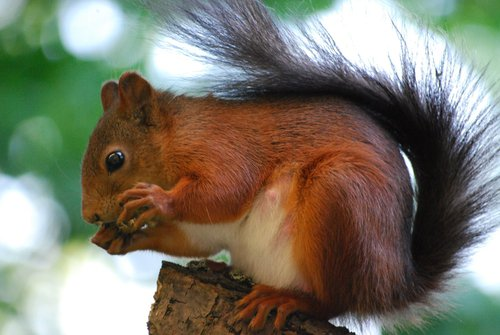
\includegraphics[width=0.8\textwidth]{images/squirrel}
  \caption[Short description]{A long description of this squirrel figure.
  Image taken from
  \url{http://commons.wikimedia.org/wiki/File:Sciurus-vulgaris_hernandeangelis_stockholm_2008-06-04.jpg}}
  \label{fig:squirrel}
\end{figure}

Citing \cite{bellard2005qfa} other documents \cite{bellard2005qfa, boileau06}
and Figure~\ref{fig:squirrel}.

Something with umlauts and a year/month date:
\cite{becher04:_feurig_hacken_mit_firew}.

And some online resources: \cite{green04}, \cite{patent:4819234}

\section{Yet Another Section}

\todo{add content}

\begin{figure}[tbp]
 \missingfigure{Come up with a mindblowing figure.}
 \caption{A mindblowing figure}
 \label{fig:todo}
\end{figure}

\section{Test commands}

\drops \LLinux \NOVA \QEMU
\texttt{memcpy}
A sentence about BASIC. And a correctly formatted one about ECC\@.

\cleardoublepage
%Additionally the combined consumption of all users makes in the first place real-pricing possible. This is instrumental for grid provider to stimulate customer using or not using their electrical device in for the grid provider convenient times. In the future will be this feature more and more necessary to avoid peaks. Through the climate crisis triggered energy transition is it highly likely that for example electrical vehicles and heat pumps are more and more components of private households. Offering the incentives to charge the car or preheating watertanks in more favorable times is only possible with a time-based pricing.
%%% Local Variables:
%%% TeX-master: "diplom"
%%% End:

\chapter{Technical Background}
\label{sec:state}

% Hier werden zwei wesentliche Aufgaben erledigt:

% 1. Der Leser muß alles beigebracht bekommen, was er zum Verständnis
% der späteren Kapitel braucht. Insbesondere sind in unserem Fach die
% Systemvoraussetzungen zu klären, die man später benutzt. Zulässig ist
% auch, daß man hier auf Tutorials oder Ähnliches verweist, die hier auf
% dem Netz zugänglich sind.

% 2. Es muß klar werden, was anderswo zu diesem Problem gearbeitet
% wird. Insbesondere sollen natürlich die Lücken der anderen klar
% werden. Warum ist die eigene Arbeit, der eigene Ansatz wichtig, um
% hier den Stand der Technik weiterzubringen? Dieses Kapitel wird von
% vielen Lesern übergangen (nicht aber vom Gutachter ;-), auch später
% bei Veröffentlichungen ist "Related Work" eine wichtige Sache.

% Viele Leser stellen dann später fest, daß sie einige der Grundlagen
% doch brauchen und blättern zurück. Deshalb ist es gut,
% Rückwärtsverweise in späteren Kapiteln zu haben, und zwar so, daß man
% die Abschnitte, auf die verwiesen wird, auch für sich lesen
% kann. Diese Kapitel kann relativ lang werden, je größer der Kontext
% der Arbeit, desto länger. Es lohnt sich auch! Den Text kann man unter
% Umständen wiederverwenden, indem man ihn als "Tutorial" zu einem
% Gebiet auch dem Netz zugänglich macht.

% Dadurch gewinnt man manchmal wertvolle Hinweise von Kollegen. Dieses
% Kapitel wird in der Regel zuerst geschrieben und ist das Einfachste
% (oder das Schwerste weil erste).

% Background Warum ist das Thema wichtig?
% Was ist das Smart Grid -> mit Background verknüpfen
% Vor, Nachteile vom Smart Grid?
% Was sind Smart Meter
% DC-Netze einführen
% Related Work: Welche andere Verfahren gibt es?
% Vllt erklärung regeln vom BSI

This section introduces an overview of the basic concepts for this work. Therefore, the key components of the smart grid are explained, what structural changes and what challenges the smart grid will bring.
In addition, this chapter discusses the current state of research.\\

\section{Smart Grid}
The original energy network was mainly considered as a transmission system to send electricity from the generators via a elongated network of cables and transformers to the consumers. Instead of a few electricity producers (e.g. nuclear power plants, coal-fired power plants), which were responsible for a large part of the electricity generation, there are now many smaller producers (e.g. wind turbines). %However, renewable power generation is often dependent on external environmental influences. Therefore, smart meters have been widely introduced in households to ensure that the smart grid is stable despite fluctuations in power generation.
However, renewable power generation is often dependent on external environmental factors. In order for the smart grid to be stable despite fluctuations in power generation, smart meters have been introduced.
This enables the electricity provider to receive the electricity consumption of a household every 15 minutes. It offers the possibility to get more easily the current electricity demand from the consumers. Previously, the current electricity demand was simulated from load forecasting models. If the demand should increase spontaneously, peaker plants, mainly consisting of coal-fired power plants, would be turned on to quickly meet this demand. This is costly and environmentally unfriendly. 
Since then, structural changes have been made to optimize the energy grid and make it more intelligent by exchanging information in near-real-time. This allows the demand to be matched to the available supply. The fundamental component of the smart grid are the smart meters, which were already mentioned. They which will be discussed in more detail in the next section.(Quelle:Smart Grid Communications)(Privacy Survey2013)

\section{Smart Meter}
Smart meters are the key component in a smart grid. A smart meter is an electricity meter that has an interface to the Internet. This enables two-way communication between the control center and the meter. This is also called Advanced Metering Infrastructure (AMI). Two-way communication improves the quality of the power grid and makes it possible to offer services that would not be possible without a smart meter. It's now possible to detect power outages. As a result, the power grid operator can detect power failures on its own. Previously, the operator was dependent on customer calls to detect power outages.
Depending on the setting, it can send electricity consumption to the electricity provider at least every 15 minutes.
hi\\
hi\\
hi\\
hi\\




\todo{write state}

\cleardoublepage

%%% Local Variables:
%%% TeX-master: "diplom"
%%% End:

\chapter{A Privacy-Preserving Aggregation Scheme Using DC-Nets}
\label{sec:design}

% Ist das zentrale Kapitel der Arbeit. Hier werden das Ziel sowie die
% eigenen Ideen, Wertungen, Entwurfsentscheidungen vorgebracht. Es kann
% sich lohnen, verschiedene Möglichkeiten durchzuspielen und dann
% explizit zu begründen, warum man sich für eine bestimmte entschieden
% hat. Dieses Kapitel sollte - zumindest in Stichworten - schon bei den
% ersten Festlegungen eines Entwurfs skizziert werden.
% Es wird sich aber in einer normal verlaufenden
% Arbeit dauernd etwas daran ändern. Das Kapitel darf nicht zu
% detailliert werden, sonst langweilt sich der Leser. Es ist sehr
% wichtig, das richtige Abstraktionsniveau zu finden. Beim Verfassen
% sollte man auf die Wiederverwendbarkeit des Textes achten.

% Plant man eine Veröffentlichung aus der Arbeit zu machen, können von
% diesem Kapitel Teile genommen werden. Das Kapitel wird in der Regel
% wohl mindestens 8 Seiten haben, mehr als 20 können ein Hinweis darauf
% sein, daß das Abstraktionsniveau verfehlt wurde.

% Die Lösung kurz vorstellen. also du hast dich für die lösung mit dem dc network entschieden und das wurde bisher noch nicht vorgeschlagen in der wissenschaft. Dann sagen bevor du das prinzip vorstellt werden erstmal alle Teilnehmer, die in dem System vorkommen, vorgestellt. dazu auch das bild aus der technischen richtlinie benutzen, wo smartmeter und smart meter admin. welche netzwerke also han etc...
%Dann sagen, dass du erstmal auf das angreifermodell eingehst und dann dc netz erklären und dann die lösung vorschlagen.
%die lösung wurde noch nicht diskutiert, weil in der wissenschaft immer davon ausgegangen wurde, dass smart meter nicht sicher sind,wir gehen davon aus, dass ein smart meter vertraut werden kann und das man deshalb auch nicht auf das billing eingehen muss, weil das smart meter korrekt arbeitet und das billing deshalb trivial ist. der stromanbieter kann auch prüfen  bzw. die logeinträge sind fälschungssicher.

%This chapter outlines the conceptual solution of this thesis to achieve privacy-preserving smart meters. The proposed protocol can be categorized as aggregation without a trusted third party[ref]. Before discussing the conceptual solution, the technical guideline from the BSI will be explained. The BSI is the cyber-security authority of the German government and is responsible for critical infrastructures such as smart grids in Germany.  The technical guideline TR-03109 resolves all security standards and security concepts that must be met by all power grid providers in Germany. Therefore, the technical guideline gives a good overview of the actual structure of the German power grid. After getting an overview of the power grid and its participants, an attacker model will be designed. The attacker model will introduce all necessary participants, what their motives are and what malicious motives they might pursue. Finally, the security protocol will be presented. It will be shown how the protocol can be integrated into the technical policy and how different potentially malicious participants are handled.

This chapter outlines the conceptual solution of this thesis to achieve privacy-preserving smart meters. The proposed protocol can be categorized as aggregation without a \gls{TTP} \ref{subsec:aggegration_without_ttp}. First, there will be a theoretical introduction to DC networks and an example to underline the theoretical concept. Subsequently, the security protocol is introduced and the functionality of the protocol is described. This includes all security mechanisms and all functions that are important for the correct execution of the protocol. In addition, mechanisms are provided to ensure the stability of the protocol in case of errors. In order to show the correctness of the protocol, the implementation of the protocol in \ref{sec:implementation} is presented and then the protocol is evaluated.

\section{A Privacy-Preserving Aggregation Scheme Using DC-Nets}
\todo{anderen Sektion Namen ausdenken}
In \cite{chaum1988dining}, David Chaum proposes a ''round-based'' protocol which he calls DC network. The DC network offers the possibility to achieve both sender anonymity and receiver anonymity in communication networks. The operation of the DC network is explained in the following section.
\subsection{DC Networks}
The DC network uses the property that any finite alphabet can be numerated( e.g a=0, b=1 etc). If an numerated alphabet from 0 is given, then this alphabet forms an abelian group regarding the addition (modulo alphabet size). The addition of the inverse element is understood as the subtraction of a character. Because of the abelian group, simple mathematical operations like addition can be performed on the numerated letters in the alphabet. 
If individual letters can be added up, then words will be also adding up as long as the words have the same length. For this reason, it is assumed that in a DC network the messages have the same length.\\
%A participant in a DC network uses one or more keys with which it superposes the messages and one generated key is then communicated to exactly one participant. 
Messages in the DC network are encrypted with a secret key to prevent a message from being traced by any participant. The principle is the same for adding up letters. For each key character, a message character is added up so that the content of the message cannot be read from the result. A generated key is shared with exactly one participant in the DC network, so that two participants use the same key to encrypt their message. These two participants are also called neighbors. For new neighbors, it is agreed that one neighbor subtracts the key and the other neighbor adds up the key. It must be considered that if there is only one neighbor in the DC network, then the neighbors can read each other's messages and no anonymity is achieved. This is because both neighbors know the key being used to disguise the messages. For this reason, a participant in a DC network exchanges a key with several neighbors. This means that nobody is able to read its neighbors messages in a DC network, because the key from the other neighbor is not known to outsiders. Thus, for each round depending on the arrangement, a message is added or subtracted with the exchanged keys by the partners. The result of the operation is distributed in the communication network and is called local superposition. 
%More precisely, each participant adds locally all key characters it generates. Then, the received keys from other participants are locally subtracted and finally, all meaningful characters (the message) that should be sent are added (modulo alphabet size) from a round. 
The distributed superpositions are added together globally and the result is transmitted back to all participants. The result is called global superposition. The global sum consists of all messages from the participants and all keys that the participants have calculated on their messages. Since each key in the global superposition has been added and subtracted exactly once\footnote[3]{As a reminder, each key is added and subtracted once precisely, because two neighbors share a key and have agreed that one neighbor will add the key and the other neighbor will subtract the key.}, the keys in the global superposition cancel out and only the meaningful messages remain. After a global superposition is distributed a round is over and a next round starts in which messages can be sent. If a participant does not want to send a meaningful message, the participant will send an empty message. This message consists only of zeros and is superposed with the key. The empty message reflects the neutral element in this structure. If all participants have sent only empty messages, the global result is a message only containing 0 for the round. If one of all participants has sent a meaningful message, the global superposition is the message for the round. If more than one participant sent a meaningful message, then the result is the total of all sent messages and a single message from the superposition cannot be recovered. The last case is also called a collision. In order to solve this problem, the collision resolution algorithm with averaging can be used in a DC network. But in this proposed protocol it is mandatory that all users send meaningful messages at the same time and that all messages form collisions with each other. %In the use case of the thesis the meaningful messages are the individual electricity consumptions of each user. Therefore the global superposition is the total power consumption of all users. From the aggregated result of all electricity consumptions it is impossible to recalculate a single electricity consumption from a individual user without major attacks on the DC Network.
\\
\\
\textbf{Key Exchange in DC Networks}
\label{subsec:key_ex}
\\
\\
Exchanging keys to calculate the local superposition can be very tedious. In addition, a different key must be exchanged for each message round. Otherwise it would be very easy to calculate the key from previously sent empty messages. Therefore, so-called pseudo-random number generators (PRNG) are commonly used. The participants share the initial values of the pseudo-random number generators with each other when they join the DC network. This can be done in the same way as the exchange of keys e.g. via a cryptographic key exchange procedure. Due to the deterministic property of PRNGs, the same number is always generated from an initial value. The result of the PRNG can be used again as a seed to produce another pseudo-random number and so forth. Therefore, for each message round in a DC network a PRNG can produce a random number after only exchanging one initial value. The random numbers are used as keys for the local superposition. This in turn means that the initial value must remain secret and must not be revealed to any other participant, since otherwise the secret keys can be found out from the initial value. The consequence would be the loss of anonymity. The security of the DC network depends largely on how secure the PRNGs are. Therefore, the PRNGs that are used must be cryptographically secure.\\
\begin{figure}[tbp]
  \centering
  \includegraphics[scale=1]{images/Schlüsselgraph.png}
  \caption[DC Network Key Graph]{A basic example of a DC network key graph\cite{stephan_escher}.}
  \label{fig:keygraph}
\end{figure}\todo{alle Bilder nochmal auflösender einfügen}
\todo{ist das wirklich vom stephan escher?}
The principle of the DC network is illustrated graphically in figure \ref{fig:keygraph} using a simple example. This visualization is also called the key graph of a DC network. A key graph is the underlying graph that is created when two participants in the DC network exchange data with each other. The users form the nodes and when two users have exchanged initial values for the PRNG, they form an edge in the graph. The example DC network shows four participants that are connected to each other along a communication link. The outer participants have only one partner, the inner participants are connected to two partners. Each participant has exchanged keys with its direct partners. The outer partners needed to exchange only one key and the inner ones exchanged keys with two direct partners.
The mathematical operation indicates whether the participant adds or subtracts the exchanged key with the partner. In the example given in the figure \ref{fig:keygraph}, the user Petra would subtract the exchanged key with Rüdiger from the message she wants to send. The result is the superposition of Petra. Rüdiger would have to add the exchanged key with Petra to his message. He would also have to subtract the key he exchanged with Sabine from the result to calculate his local superposition. After everyone in the network has calculated their local superposition, all local superpositions are distributed to every user. Subsequently, every participant in the DC network can calculate the global superposition from all local superpositions \cite{stephan_escher}\cite{pfitzmann2006security}.

%peusodzufallsgeneratoren
\section{DC Network Protocol in a German Smart Grid}
The DC network is a scheme that can be used to achieve sender anonymity and receiver anonymity. Considering the use case of the thesis, the receiver anonymity does not have to be implemented. Since the aim is to anonymize the electricity consumption of a customer and send it to the electricity provider. In this case, the electricity provider is a public recipient and known to all participants. Therefore, the identity of the electricity provider does not need to be protected. Unlike in a normal DC network, in the proposed solution the participants do not want to communicate with each other, they only want to send their electricity consumption to the electricity provider. Therefore, the global superposition does not have to be distributed in the network but only has to be calculated at the electricity provider. The only exception is when joining or exiting the DC network.
During the registration process the \gls{SMGW}s have to perform a key exchange to configure the initial value for the PRNG as explained in \ref{subsec:key_ex}. Before introducing the core functions of the network protocol, it is described how the protocol can be arranged with the \gls{TR-03109} of the \gls{BSI} \cite{TR-031}.\\
\\
\textbf{Compatibility with the TR-03109}
\\
\\
\begin{figure}[tbp]
  \centering
  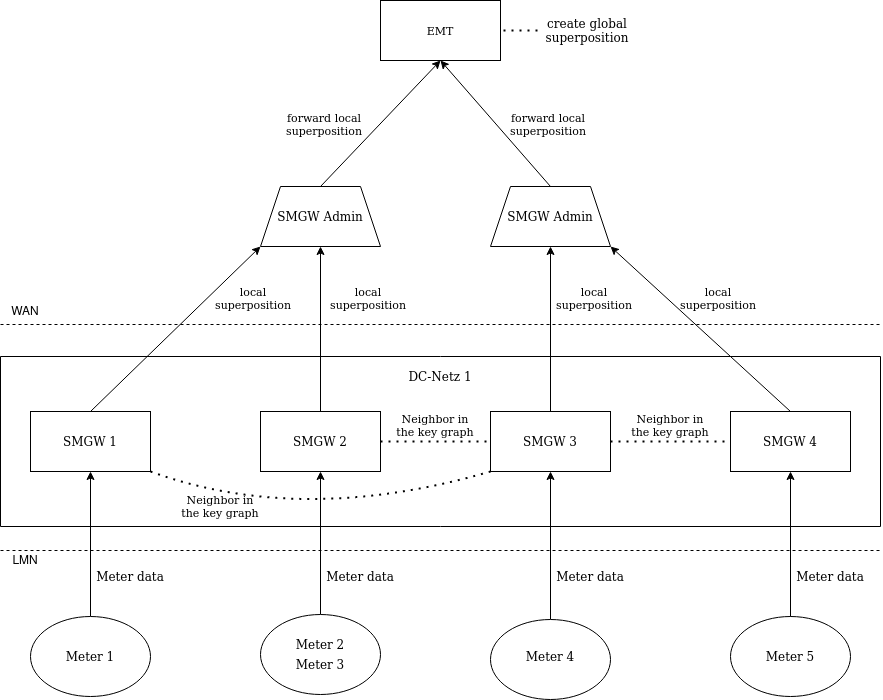
\includegraphics[width=1\textwidth]{images/Top-down_update.png}
  \caption[DC Network Compatibility with TR]{
In the figure, the 6 components of the DC network frame are
are shown.}
\label{fig:top_down}
\end{figure}\todo{In English}The DC network must be compatible with the installed infrastructure. Otherwise, the design would not be implementable and impractical for real-world use. Therefore, a large part of the requirements from the \gls{TR-03109} were taken into account in the creation phase of the design.\\ In Figure \ref{fig:top_down}}, it can be seen how the DC network is integrated into the stakeholder model of the \gls{TR-03109}. In addition, the interface boundaries of \gls{LMN} and \gls{WAN} for the different stakeholders are drawn. The design shows that the DC network protocol needs to be implemented only on the \gls{SMGW}s. No structural changes need to be made. According to the \gls{TR-03109} from the \gls{BSI}, \gls{SMGW}s are only allowed to communicate with authorized participants in the smart grid and all foreign requests are ignored. These are \gls{EMT}s, \gls{GWA}s and the electricity provider. But it is not possible for two \gls{SMGW}s to establish a communication link with each other, because \gls{SMGW}s are not authorized participants in the power grid. Therefore, it is necessary for electricity provider to take over administrative tasks, e.g. to provide necessary communication tunnels for \gls{SMGW}s to each other. Additionally, the electricity provider is storing the key graph so that possible errors on the DC network can be corrected and assure stability.\\ %In this design, careful consideration has been given to the rights of the electricity provider to ensure a stable DC network. \subsec:stakeholder_model
A message round in the stakeholder model in combination with the DC network looks as follows. As a comparison sending the power consumption without DC network was described in \ref{subsec:stakeholder_model}. The \gls{SMGW} receives the power consumption data from the meters of the different houses. The \gls{SMGW} implements the communication profiles configured by the \gls{GWA}. Despite the implementation of the DC network, there is no impact on the processing of the data in the \gls{SMGW}, since the DC network is performed only after the application of the communication profiles as it can be seen in \ref{fig:value_processing_with_dc}. The creation of the local superposition is the last processing point before sending the DC network protocol data to the electricity provider. The local superposition is then forwarded to the electricity provider via the \gls{GWA}. Although the \gls{GWA} is between the electricity provider and the \gls{SMGW} during the transmission of the data, the \gls{GWA} only forwards the data and does not perform any operations or process the protocol data. Therefore, the \gls{GWA} will not be considered further in the protocol below.\\ The electricity provider\todo{Electricity PRovider anstatt emt} then calculates the global superposition from all local superpositions. In the use case of the thesis the meaningful message contained in the local superposition is the individual electricity consumption of a customer. Therefore, the calculated global superposition is the total power consumption of all users in the DC network. In addition, \gls{SMGW}s send their electricity consumption to the electricity provider every 15 minutes. A round-based network for anonymizing content data like the DC network is particularly suitable for achieving privacy in a smart grid with high transmission intervals.
%In the use case of the thesis the meaningful messages are the individual electricity consumptions of each user. Therefore the global superposition is the total power consumption of all users. From the aggregated result of all electricity consumptions it is impossible to recalculate a single electricity consumption from a individual user without major attacks on the DC Network.
%The design aligns with the existing stakeholder model in the technical guideline. Additionally, only the DC network protocol needs to be implemented. The exact implementation of the protocol is described starting in the next paragraph. \\
\\
\textbf{Protocol Header}
\\
\\\begin{figure}[tbp]
  \centering
  
\includegraphics[width=1\textwidth]{images/Header.png}
  \caption[DC Network Frame]{
In the figure, the 6 components of the DC network data package are
are shown.}
  \label{fig:frame}
\end{figure}\todo{Protocol Identifier}In the network protocol messages are sent via data packages. The structure of a package in the DC network protocol is shown in the figure \ref{fig:frame}. Each package consists of a small header and the data part in which usually the local superposition is transfered. The purpose of each field is described further below.\\
The first field is the Protocol Identifier field. The purpose of the Protocol Identifier field is to ensure that the application of the DC network protocol is recognized by all participants and that the \gls{SMGW}s as well as the electricity provider can react correctly to the packages. This is followed by the DC Network Identifier field.%muss ich das hinschreiben?
The DC Network Identifier field offers the electricity provider the possibility to operate several DC networks in different regions and to distinguish DC networks. In addition, each \gls{SMGW} is given a unique identifier so that the \gls{SMGW}s in a network can be distinguished. If the network needs to perform an error correction, \gls{SMGW}s can be notified by the identification number from the power supplier. Although the \gls{SMGW}s can be identified by the field, the electricity provider still cannot draw any conclusions about electricity consumption from the local superposition. The Transmission Bit indicates that an \gls{SMGW} has sent a local superposition to the electricity provider in a round. Furthermore, it is used for error correction procedures. The Time Stamp field indicates when a message was sent by a participant. This allows the electricity provider to classify messages by round and not mix up for messages from different rounds. The next field is the Notification field. The field is used for correction procedures or notifications for certain operations. An overview of all notification codes is presented in table 3.1. The electricity provider can thus send notifications to the \gls{SMGW}s to start error correction procedures. In the last field, the Data field, only the local superpositions are sent. The \gls{SMGW}s do not transmit any information other than the power consumption in the Data field. Therefore, it can be assumed that rather small messages are sent with the proposed protocol.\\
\\
\textbf{Protocol Initialization}
\\
\\
For the Protocol Initialization it is assumed that the electricity provider wants to create a new empty DC network. In order to achieve this a few preparations have to be made. First, a unique and unchangeable DC Net Identifier is assigned from the electricity provider to the empty DC network. At least 2 \gls{SMGW}s have to enter the DC network. A DC network with only one participant is not operational and cannot offer anonymity. 
The \gls{SMGW}s that enter the network are assigned a Client Identifier by the electricity provider.\\
%vllt woander hin schreiben
To ensure a minimum level of protection for participants in the DC network, the DC network must have a minimum number of users. Even if the electricity provider receives aggregated electricity consumption, individual households may be more noticeable. Different house sizes and number of people in a household can lead to a significantly higher electricity consumption, which is visible in the aggregated result for small DC networks. In this master thesis, a stochastic analysis is performed in the experiments chapter \ref{sec:experiments} to determine a minimum number of participants. It is assumed that in the DC network each participants has at least 3 connections to neighbors. This reduces the risk of individual \gls{SMGW}s being disconnected from the DC network or malicious neighbors being able to reconstruct the power consumption from the local superposition.\\
%According to the Technical guideline TR-03109 from BSI, \gls{SMGW}s are only allowed to communicate with authorized participants in the smart grid and all foreign requests are ignored. These are EMTs, GWAs and the electricity provider. %But it is not possible for two SMGWs to establish a communication link with each other, because SMGWs are not authorized participants in the power grid. In order for the DC network to become operational, two SMGW must exchange an initial seed value to configure the PRNGs. Therefore, it's necessary for electricity provider to take over administrative tasks and provide tunnels for key exchange as described in \ref{subsec:key_ex}. Additionaly the electricity provider is storing the key graph so that possible errors on the dc network can be corrected and assure stability by an entity. In this design, careful consideration has been given to the rights of the electricity provider to ensure a stable DC network.
In order for the DC network to become operational, two \gls{SMGW} must exchange an initial seed value to configure the PRNGs. %When a start value is exchanged, both PRNGs of the clients are initialized. 
As a result, the same random number sequences would be generated independently of each other by the PRNG on both clients. But there is a current communication barrier that does not allow \gls{SMGW}s to communicate with other \gls{SMGW}s. With the limited communication capabilities, the \gls{SMGW}s rely on the electricity provider. The electricity provider must provide a tunnel for the \gls{SMGW}s so that the \gls{SMGW}s can communicate with each other and exchange the start seed for the PRNG. The tunnel works as follows. An \gls{SMGW} receives the tunnel information by the power provider. The \gls{SMGW} can then send messages to the tunnel of the power provider. When messages arrive at the tunnel, the power provider forwards the messages to the receiving \gls{SMGW}. Of course, the electricity provider has the technical possibility to eavesdrop on the tunnel. For this reason, secret information such as the start value of the PRNG must be exchanged in a cryptographically secured procedure via the tunnel. One method to securely exchange the start value would be the Diffie Hellman key exchange.\\
\begin{figure}[tbp]
  \centering
  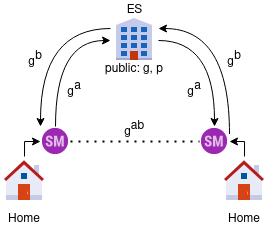
\includegraphics[scale=0.7]{images/key_exchange.png}
  \caption[Diffie-Hellman Key Exchange in TR-03109]{The Diffie-Hellman key exchange between two SMGWs via a electricity supplier \gls{ES}.}
  \label{fig:keyexchange}
\end{figure}
%vllt noch den tunnel einzeichnen im diagramm?
Diffie-Hellman is a known key exchange protocol, where two users can publicly exchange a secret over a unsecure channel without a third person being able to figure out the secret. 
Diffie-Hellman requires a generator $g$ and a prime $p$, and the two values are public to all users. If two users want to exchange a key via Diffie-Hellman, then both users choose a secret random number a that is between $1$ and $p-1$. Each user calculates the public key $ka$ by $ka=g^a$. The public key is distributed to the partner and at the same time the partner's public key $kb=g^b$ is obtained, where $b$ is the random number between $1$ and $p-1$ of the partner. After obtaining the public key, both users can calculate $kab=g^{ab}$.%\begin{equation}
%\label{eq:abc}
%kab=g^{ab}
%\end{equation}
Even if an attacker could eavesdrop on the values $g^a$ and $g^b$, he would not be able to compute $g^ab$ because the computation of the discrete logarithm problem cannot be performed efficiently. How the Diffie-Hellman key exchange is executed in the smart grid use case is shown in Figure \ref{fig:keyexchange}. 
%fußnote. natürlich ist in der kommunikation zwischen sm und es noch der gwa, der aber vernachlässigt werden kann, da der nur die daten weitersendet zum es.
Both \gls{SMGW}s receive their public generator and prime number from the electricity provider. Then, $g^a$ and $g^b$ are calculated and sent to the partner via the electricity provider's provisioned tunnel. Afterwards, $g^ab$ can be calculated by both \gls{SMGW}.\\
\gls{SMGW}s can generate cryptographically secure keys because they have a hardware security module built in. Therefore, key exchange procedures such as Diffie-Hellman can be executed for the \gls{SMGW} without any problems. Diffie-Hellman was also only mentioned as an example. There are various attacks on the presented textbook Diffie-Hellman variant.\todo{quelle}
The forwarding of \gls{SMGW} messages by the electricity provider enables the implementation of other substantially secure key exchange procedures. The advantage of this approach is that \gls{SMGW}s are anonymous to other \gls{SMGW}s. When the keys are exchanged, only the partners with whom the key is currently exchanged are aware of it. Uninvolved \gls{SMGW}s do not receive any information about the entry of new users in a DC network. Furthermore, a \gls{SMGW} can generally obtain little information about other participants in the DC network since it can not communicate directly to other \gls{SMGW}s. But the participants share their Client Identifiers during the key exchange in the registration process. Due to the exchanged communication details, each participant in the DC network knows the identification number of its neighbor. This is helpful later for error correction measures. %Vllt angriffe nach dem Kapitel SChreiben?
\\The use of a key exchange method also involves risks. By forwarding messages, the electricity provider knows which \gls{SMGW} have exchanged keys with each other. Exchanging keys is equivalent to creating an edge in the key graph. %referenz hinzufügen als ich keygraphs erklärt habe
Therefore, a malicious electricity provider can easily perform an active attack on single \gls{SMGW}s with the knowledge of the structure of the key graph. %the key graph of the DC network. The knowledge about the structure of the key graph alone does not give the electricity provider any further knowledge, but a malicious electricity provider could use the knowledge to launch active attacks on individual \gls{SMGW}. 
An example would be that if a electricity provider wants to get information about the power consumption of a \gls{SMGW}. The electricity provider could connect one or more \gls{SMGW}s it controls to the victim \gls{SMGW} through a key exchange that the attacker \gls{SMGW} launches. The electricity provider could now hope that in the future the victim \gls{SMGW} will only have keys with the attacker \gls{SMGW}s. Since the electricity provider controls the attacker \gls{SMGW} and knows the keys of the attacker \gls{SMGW}, it can reconstruct the electricity consumption of the victim \gls{SMGW} from the local superposition. To counter the introduced attack, participants must have a minimum number of neighbors. The more neighbors a \gls{SMGW} has, the smaller the chance that each neighbor is a malicious attacker. Moreover, the electricity provider would have too much power in the DC network if it can control which \gls{SMGW}s connect to each other upon entry. Therefore, a joining \gls{SMGW} must be assigned to a random partner in the DC network.\\ %Furthermore, in order for error correction measures to be implemented as easily as possible, the underlying key graph in the DC network must be planar.\todo{hier nochmal drüber schauen}\\
\\
\textbf{Bootstrap Phase in a DC Network}
\\
\\
\begin{table}
\centering
\adjustbox{max width=\textwidth}{
	 \begin{tabular}{|c|c|}
	\hline
	Notification Description & Functionality\\
	\hline 
	Notification 1 & A SMGW wants to register in a DC Network\\ 
	\hline
	Notification 2 & A SMGW has succesfully entered a DC Network\\
	\hline
	Notification 3 & Electricity provider informs SMGW that its neighbor is leaving the DC network\\
	\hline
	Notification 4 & Resent local superposition according to the correction procedure\\
	\hline
	Notification 5 & Transmitting local superposition\\
	\hline
	Notification 6 & Former defective DC client is rejoining the DC network\\
	\hline
	Notification 7 & An SMGW informs the electricity provider that it is leaving the DC network \\
	\hline
	\end{tabular}}
	\caption[Notification Description List]{An overview of all notification messages.} 
	\label{img:notification}
\end{table}
\begin{figure}[tbp]
  \centering
  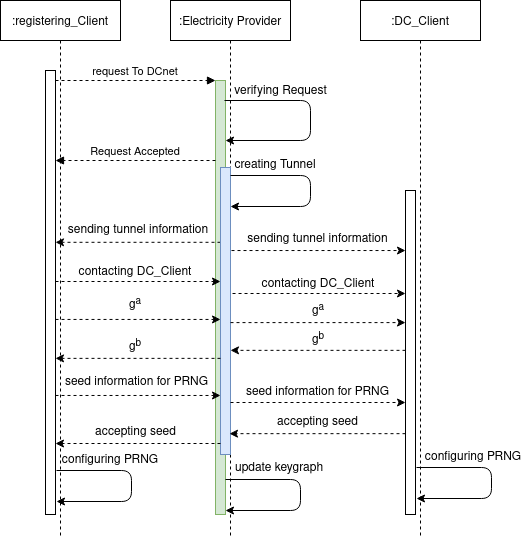
\includegraphics[width=0.8\textwidth]{images/Registering2.png}
  \caption[Sequence Diagram Registering]{
A sequence diagram showing the functions for registering an SMGW in a DC network.}
  \label{fig:sequencediagramregistering}
\end{figure}
A \gls{SMGW} that wants to register in the DC network sends a special defined request to its power provider. For this purpose the notification field in the header is used and notification 1 is sent. Notification 1 represents a request from the \gls{SMGW} to register in a DC network. The electricity provider assigns the requesting DC client to a suitable geographical region and suggests a random DC client (\gls{SMGW}) which is already registered in the DC network. Afterwards the electricity provider establishes a tunnel and sends the tunnel information to the DC client and the registering client. Via this tunnel it is possible for the two \gls{SMGW}s to create a communication link via the electricity provider. If an \gls{SMGW} sends to the tunnel, the message is forwarded to its future neighbor. The DC client which is already present in the DC network is only informed by the electricity provider that it receives a new neighbor and has to exchange contact information. The requesting \gls{SMGW} needs to send the seeds for the PRNG over the tunnel. To prevent the electricity provider from reading the seeds, the clients swap the seed secured by the Diffie-Helmann key exchange through the tunnels provided.\\%ist das korrekt?
Once the seeds have been exchanged, the power provider is informed by the requesting client that it has successfully entered the DC network by\todo{wie wird die lokale summe verifiziert?} notification 2. The PRNGs are now configured and the generated keys can be added or subtracted to the message in order to create the local superposition. The procedure is explained in more detail in paragraph \ref{subsec:key_ex}.%erklärung zu PRNGs
The communication exchange between all participants in the registration process of a DC network is graphically illustrated in Fig \ref{fig:sequencediagramregistering}. %nochmal diagram anpassen.
Afterwards all participants in the DC network can send their local superpositions to the power provider. The provider forms the global superposition and receives the aggregated power consumption of all \gls{SMGW}s in the DC network. If necessary, the electricity supplier must ensure that in the future messages can continue to be exchanged between registered customers via the same tunnel. In addition, already registered clients can not choose which new communication partners they get. Furthermore, it is assumed that the electricity provider has already been authorized by the \gls{GWA}. Otherwise, the \gls{SMGW} would not be able to establish a connection to the supplier.\\
%(der Gedanke ist, dass es viele verschiedene kleine DC-Netze gibt, die getrennte Schlüsselgraphen besitzen, jedes DC-Netz sendet seine lokale Summe an den Stromanbieter, der alle Werte aufsummiert und die globale Summe bildet (für ein DC-Netz)
\\
\textbf{SMGW Regular Operation}
\\
\\
%wie sieht eine normale Operation aus? wie häufig wird gesendet? wofür wird das transmisson bit verwendet? und der timestampt
So far, the steps to initialize a DC grid into the already operating power grid have been explained. Next, a description is given of how the technical process takes place in the DC grid, assuming that no faults occur or corrective measures need to be taken. The \gls{SMGW} transmits its electricity consumption periodically from the moment it enters the DC network. The transmission interval for the electricity consumption is 15 minutes. Hence, for the DC network, it is most practical if all \gls{SMGW}s send their local superposition to the power supplier at the same time or within a short transmission interval (e.g. one minute). This can be done without problems, because according to ref 3.1 all \gls{SMGW} must update their time in regular intervals with NTP servers. If an \gls{SMGW} has not sent a local superposition within the transmission interval, corrective measures are implemented. The packet that a \gls{SMGW} sends to the power provider is filled in as follows:
\begin{enumerate}
\item DC Net Identifier:\\
The DC net in which the \gls{SMGW} is registered is entered here.
\item Client Identifier:\\ 
The assigned Client Identifier is sent in this field.
\item Transmission Bit:\\
This field is exactly 1 bit and is set to 1 when a local superposition is sent.
\item Time Stamp:\\
A time stamp is appended when the frame is generated.
\item Notification:\\
Notification message 5 is sent to inform the electricity provider that this message is a local superposition.
\item Data:\\
Generated local superposition is entered in the data field.
\end{enumerate}
The electricity provider processes the received frames according to the following procedure:\\
\begin{enumerate}
\item DC Network Identifier:\\
DC Network Identifier indicates to which DC net the message is processed.
\item Client Identifier:\\
The Client Identifier of the package is stored in a memory structure. The memory structure shows, which client has not sent a local superposition in the round.
\item Transmission Bit: Each message has a transmission bit set to 1. All transmission bits are added up and at the end of the round it can be checked whether all \gls{SMGW}s have sent their local superposition. If the summed transmission bits do not correspond to the number of participants in the DC network, correction procedures must be applied.
\item Time Stamp: The power supplier can assign the message to the correct round.
\item Notification: Notification message 5 informs the electricity supplier that the local superposition is being transmitted.
\item Data:
The local superposition in the field is added up with all other superpositions and the electricity provider gets the global superposition. This is the aggregated power consumption of all \gls{SMGW}s in the DC network.
\end{enumerate}
\\
\\
\textbf{Teardown Phase in the DC Network}
\\
\\
\begin{figure}[tbp]
  \centering
  \includegraphics[width=0.8\textwidth]{images/Exit.png}
  \caption[Sequence Diagram Exiting]{A sequence diagram showing the functions for a SMGW, which wants to exit a DC network.}
  \label{fig:Exit}
\end{figure}
An exit can be caused, for example, when the customer changes the electricity provider. Then a notification message 7 is sent from a \gls{SMGW} to the electricity provider, which informs the electricity provider about the exit of the \gls{SMGW}. The electricity provider instructs the neighbors of the exiting client with a notification message 3. The electricity provider may not abuse Notification 3. Otherwise, a malicious electricity provider would be able to change the structure of the DC network at will. Hence, the misuse must be prevented technically, since the exit from the DC network is one of the standard functions and it is difficult per design to prevent a misuse of standard functions.\todo{per design... ist das ok?} In addition to the notification message 3, the DC Client Identifier of the exiting \gls{SMGW} is sent as well. This notification signals to the neighbors of the exiting \gls{SMGW} that they must discard their PRNG configurations to client $X$ and that they must not be used in the calculation of the local superposition in the next round. In order to avoid a synchronization error in the DC network, the "neighbors" must confirm to the power provider that the configuration has been discarded. Otherwise the case may occur that a \gls{SMGW} continues to add the old key to its message. This would result in a useless global superposition.\\ Furthermore, the key graph must be considered. It could happen that the underlying key graph splits into two DC networks. In this case, two separated DC networks are sending to the same DC network identifier. In the example of Figure \ref{fig:keygraph}, the scenario could occur if Sabine and Rüdiger throw away their shared key. The result is different depending on the position where a DC net splits. But at least one DC network experiences a significant loss of anonymity due to the smaller number of participants that can be aggregated. In the case of particularly serious splits, it can even lead to a participant being completely disconnected from the DC network. If a disconnected client notices that it no longer has any neighbors, it sends a special emergency message to the power provider. Then a new registration process is initiated before the next round starts.\\ To avoid splitting into two DC networks, the exiting \gls{SMGW} informs its neighbors with which direct partners it was connected. These then initiate a registration process and exchange keys with each other. The fact that all neighbors have exchanged keys with each other guarantees that a DC network does not split when an \gls{SMGW} leaves.\\ Furthermore, all participants have to have a minimum number of 3 neighbors. This makes the possibility of disconnection from the DC grid much less likely, since several neighbors would have to leave the DC grid at the same time for a participant to be exposed. In the sequence diagram in figure \ref{fig:Exit} it is shown which communication exchange is performed so that an \gls{SMGW} can leave the DC network.
\section{Error Correction Procedures}
\label{error_corr}
It was described how DC networks work and how a DC network works in a normal operation without interference. This section explains which attacks on the network are possible and how the DC network deals with potential disturbances.
\\
\\
\textbf{SMGW Connection Loss}
\label{error_corr_conn}
\\
\\
\gls{SMGW} can access the Internet by communicating over their \gls{WAN} interface. If the Internet connection is interrupted, this can lead to an \gls{SMGW} not being able to send its local superposition in time. The result is that the electricity provider cannot calculate a meaningful global superposition in the round. The electricity provider notices the error immediately because the global transmission bit does not correspond to the number of participants in the DC network. In this case, the following corrective actions are implemented:\\ %vllt noch gliedern in 1. locate errorneous client 2. korrektur via local sum 3. save keys von client 4. restore keygraph when client is back up
The electricity provider detects which \gls{SMGW} has not sent a local superposition based on the Client Identifier. Since the \gls{SMGW} sends a complete header and the Client Identifier of an \gls{SMGW} is also sent underneath, an electricity provider only has to check which Client Identifier was not sent. The missing Client Identifier is also the client that is defective. Once the defective client is located, notification 4 is sent by the electricity provider to the neighbors of the defective client. The notification contains the Client Identifier of the defective client and requests the neighbors to recalculate their local superposition, but without using the key of the defective client. Afterwards the updated local superposition is resent to the electricity provider. Even though the first attempt failed the electricity provider can calculate a meaningful global sum by using the resent local superposition instead of the old local superposition. At the same time, the keys of the defective client are stored by the neighbors in a backup, so that when the defective client re-enters the DC network, the same key graph is restored. The neighbors of the defective client experience no loss of anonymity during the correction process.\\%vllt noch schreiben weil jeder client mehr als eine verbindung hat
After this procedure, the defective client is temporarily no longer in the DC network. As soon as the \gls{SMGW} obtains an Internet connection, it rejoins in the DC network by sending a Notification 6 to the electricity provider. Thereupon the electricity provider informs the neighbors that in the next round the key of the former faulty neighbor is to be reused for the calculation of the local superposition. The power consumption of the \gls{SMGW} during the time of Internet loss is not retransmitted. This is because retransmission of the power consumption would lead to a complete loss of anonymity. The electricity provider knows at which time stamp which smart meter was defective and could assign the resent electricity consumption directly. Furthermore, the electricity provider knows how many smart meters are functional at any time and how many are defective through the transmission bit. Therefore, the electricity provider can evaluate how conclusive the data is in the DC network. %and the assigned number of participants in the DC network. 
If not a larger amount of participants of the DC network fails, the electricity provider is still able to ensure a good network stability. %Especially since the chance of an Internet outage is unlikely. 
In addition, an Internet loss does not have an impact on the billing of a \gls{SMGW}, because the calculation of the billing is executed via another procedure on the \gls{SMGW}. Therefore, the electricity provider does not have to fear any loss of income, even though the electricity consumption is not sent.\\
\\ 
\textbf{Manipulation of the Local Superposition}
\label{subsec:mani_local}
\\
\\
\begin{figure}[tbp]
  \centering
  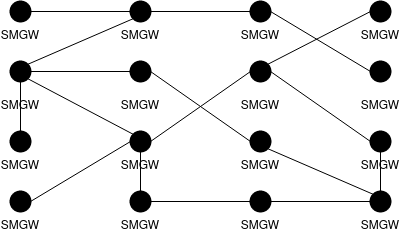
\includegraphics[width=0.5\textwidth]{images/DC Net before Split.png}
  \caption[Example DC Network]{An example of a DC network before it is split in the algorithm. The edges between the nodes represent a PRNG configuration.}
  \label{fig:splitDCNetwork}
\end{figure}One of the considerations that absolutely must be made in a DC network is: What happens if an \gls{SMGW} intentionally manipulates its local superposition?\todo{dieser satz korrekt?}\todo{planar reinnehmen oder nicht reinnehmen?}
First of all, it must be mentioned that this attack does not help the customer at all to avoid the electricity costs. This is because the electricity costs are calculated by a separate procedure and therefore the billing cannot be affected by the attack.\\ If this problem does occur, it should rather be assumed that it is an external attacker who has taken over an \gls{SMGW} and wants to sabotage the availability of the DC network.
If the local superposition is manipulated, e.g. by deliberately sending a wrong local superposition, it is no longer possible for the electricity provider to calculate a meaningful global superposition. Hence, it is not possible to see the aggregated power consumption for the whole DC network. In the case of the attack, the electricity provider cannot assume that the situation will resolve itself and must take measures to find the manipulating \gls{SMGW}. Furthermore, it must be assumed that the attacker is well aware that the electricity provider will be looking for him. Therefore, the procedure must be designed in such a way that the attacker is found even though he tries to conceal his identity.\\
For this purpose, a slightly modified version of Pfitzmann's error localization and recovery protocol can be applied \cite{pfitzmann2006security}. The protocol of Pfitzmann describes 2 different modes, the anonymity mode (A-Mode), in which the DC net works normally and the fault tolerance mode (F-Mode), in which defective stations are searched for .
The F-mode can be extended in this application so that an attacker can also be searched for. If there is an incorrect calculation in the global superposition and no \gls{SMGW} is having Internet issues, this is communicated publicly by the electricity provider to the \gls{SMGW}s. All \gls{SMGW}s then save the keys and the electricity consumption from the last round. At the same time the electricity provider saves all receiving local superpositions from the round and enjoys special rights that only prevail in F-mode. The figure \ref{fig:splitDCNetwork} shows an example DC network to illustrate how the proposed algorithm works.\\
In the following, an algorithm exploits a property of DC networks that allows a DC network with one meaningful global superposition to separate into two DC networks with two separate meaningful global superpositions.
After a round is manipulated by an active attacker, the DC network is halved and the failed round is repeated with the same configurations and power consumption. Since the hole round is repeated every participant including the attacker has to resend the same local superposition from the failed round. Since there are now two DC networks, a global superposition will be meaningful and the other global superposition will be unreadable. 
This allows the electricity provider to narrow down the attacker, since the attacker will always be located in the DC network where the calculation of a meaningful global superposition fails.\\
The algorithm is executed in four steps:\todo{hier weitermachen}
\begin{enumerate}
\item Halve the key graph. 
The power provider has the overview of the key graph and can therefore separate the key graph into two parts. %Splitting the graph into two halves should be trivial since the planar separator theorem holds.
\item If a \gls{SMGW} is exactly on the border of the bisected key graph and has a neighbor in the other half of the key graph, then this \gls{SMGW} is informed as a border node by the power provider that the neighbor's key is thrown away for this computation.
\end{enumerate}
The temporary throwing away of the keys leads to the splitting of the key graph at that point. The power provider can request an \gls{SMGW} to throw away a key only in F-mode, because throwing away a key of a neighbor immediately weakens the anonymity of an \gls{SMGW}. 
\begin{enumerate}[resume] 
\item All SMGWs in one half of the key graph now retransmit the local superposition from the last failed round. 
\end{enumerate}
The border \gls{SMGW}s that threw away a key, calculate the new correct local superposition without the key of the neighbor in the other part of the key graph. This procedure results in all nodes sending the same message from the last round except the border nodes and allows two global superposition to be calculated. One global superposition from the first half and one global superposition from the second half of the DC network. So the old DC network round is repeated, but in a split net to reduce the number of possible attacker \gls{SMGW}. The electricity provider can check by the stored local superposition if the same local superposition is really resent and can check the correctness in a resent round. 
\begin{enumerate}[resume]
\item If the calculation of a global superposition fails in the first half of the DC network, then the attacker will be located in the first half and the first half is separated again in two halves. If the calculation of a global superposition fails in the second half of the DC network, then the attacker will be located in the second half and the second half is separated again in two halves. If the global superposition fails in both halves or is calculated correctly, then the attacker will be among the border nodes.
\end{enumerate}
The procedure is continued recursively until it is reduced to one \gls{SMGW} that is eligible to be the attacker. The figure \ref{fig:FirstSplitting} shows the first step of the DC network splitting algorithm.
There can be the special case that the attacker \gls{SMGW} is a border node. Since the border nodes send a recalculated local superposition, the power provider cannot immediately rule out whether the attacker is among the border nodes. Therefore, for each bisection, an additional subgraph must be formed in which the former border nodes have no neighbors outside the subgraph. In this way it is possible for the electricity provider to control the local superposition when resending the local superposition of the former border nodes. \\
Since the power provider is granted extended rights in F-mode, it must be ensured that the power provider does not abuse F-mode by, for example, running the DC network in F-mode all the time. To prevent misuse, all \gls{SMGW}s in the DC network must be informed at all times as to which mode the DC network is in. If the DC network is conspicuously often in F-mode, this could be an indication that the electricity provider is abusing its rights. In this case, the \gls{SMGW}s have the option to leave the DC network and terminate the contract with the electricity provider.
\begin{figure}[tbp]
  \centering
  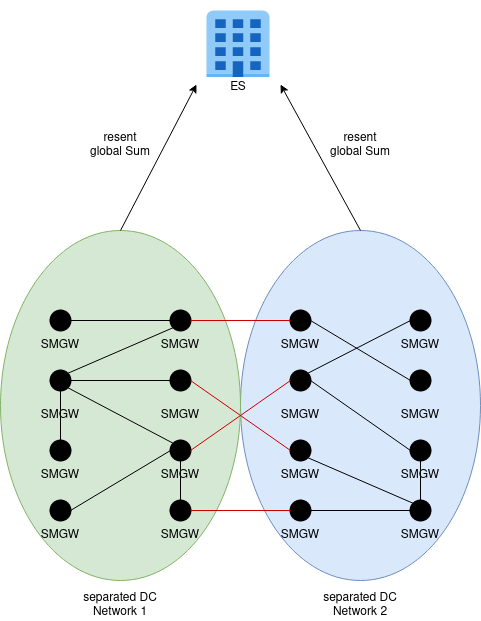
\includegraphics[width=0.5\textwidth]{images/DC Net Split.png}
  \caption[DC Network Splitting Algorithm]{The result of the first division of the DC network in F-mode. Red edges are division edges removed from the original network.}
  \label{fig:FirstSplitting}
\end{figure}
%was passiert mit den Sonderknoten? wie wird mit den 3 kanten umgegangen, aber man hat ja am ende nur 2 \gls{SMGW}?
%lsg größere gruppe mit der der angreifer identifiziert wird.
%also wenn nur noch 2 in frage kommen, werden diese beiden in eine größere gruppe gesteckt und geschaut, ob die größere gruppe falsch ist.
\\
\\
\textbf{DC Network Size}
\\
\\
With a small number of participants, conclusions can be drawn about individual participants from the aggregated result. This is the case if the electricity consumption of one user is equal in percentage to the residual consumption of the other users. Or it is also feasible that a user does not consume any electricity. In a DC network with 2 users, the power consumption would be directly readable even if the individual loads are aggregated. The goal is not to avoid the disclosure of information, but rather to make it hard to draw inferences about an individual user from the aggregated consumption \cite{le2020differential}.
In this thesis, the experiments chapter determines the minimum size of a DC grid to guarantee that statistical inferences are difficult to realize.
On the other hand, it is in the interest of the power supplier not to realize huge DC networks. The more participants a DC network has, the more frequently errors occur that have to be corrected by corrective measures. Although the DC network should scale with many participants, the question arises as to how meaningful the results are when hundreds of participants partially fail.%Etwas über die Größe schreiben, dass die DC netze nicht zu klein sein dürfen, aber es auch vorteile bringt, wenn sie nicht zu groß sind.
%vllt noch schreiben wie das in die technische Richtlinie implementiert werden könnte?


%noch unbedingt schreiben, dass in dem Protokoll unbedingt gewollt ist, dass es zu kollisionen kommt und das in einem normalen DC netz kollisionsauflösungsverfahren angewendet werden. siehe überlagerndes empfangen


\section{Implementation}
\label{sec:implementation}
% Hier greift man einige wenige, interessante Gesichtspunkte der
% Implementierung heraus. Das Kapitel darf nicht mit Dokumentation oder
% gar Programmkommentaren verwechselt werden. Es kann vorkommen, daß
% sehr viele Gesichtspunkte aufgegriffen werden müssen, ist aber nicht
% sehr häufig. Zweck dieses Kapitels ist einerseits, glaubhaft zu
% machen, daß man es bei der Arbeit nicht mit einem "Papiertiger"
% sondern einem real existierenden System zu tun hat. Es ist sicherlich
% auch ein sehr wichtiger Text für jemanden, der die Arbeit später
% fortsetzt. Der dritte Gesichtspunkt dabei ist, einem Leser einen etwas
% tieferen Einblick in die Technik zu geben, mit der man sich hier
% beschäftigt. Schöne Bespiele sind "War Stories", also Dinge mit denen
% man besonders zu kämpfen hatte, oder eine konkrete, beispielhafte
% Verfeinerung einer der in Kapitel 3 vorgestellten Ideen. Auch hier
% gilt, mehr als 20 Seiten liest keiner, aber das ist hierbei nicht so
% schlimm, weil man die Lektüre ja einfach abbrechen kann, ohne den
% Faden zu verlieren. Vollständige Quellprogramme haben in einer Arbeit
% nichts zu suchen, auch nicht im Anhang, sondern gehören auf Rechner,
% auf denen man sie sich ansehen kann.




% Also kurzer Überblick über die Struktur schreiben, dann auf GRPC eingehen. Wenn GRPC erklärt wurde, würde ich den DC_rounds Service vorstellen. Dann pseudoartig auf die Funktionen eingehen und ein Diagram zeichnen.
%Wo gab es probleme bei der implementation? Es gab probleme bei der synchronisation der unterschiedlichen teilnehmer.-> unterschiedliche Sekunden. Außerdem war es neu, dass mehrere nutzer auf den selben servercode "zugreifen" und das parallele programmieren. die fork nicht vergessen.
% wo gibt es unterschiede? design von grpc eingehen, man kann keine Nachrichten weiterleiten mit grpc. Nur 2 verbindungen zwischen CLients möglich.vllt noch mehr?
The conceptual approach of the DC network was presented above. Nevertheless, smart grids are a real-world system and it must be shown that the theoretical solution can be implemented in a practical environment. This section deals with the implementation of the introduced DC network protocol. It is described which technical tools were used and where implementation problems occurred.
\subsection{Structure of the Testbed}
%In the practical Implementation in this work it was tried to implement a DC network with the same requirements as de
In the practical implementation in this work it was tried to implement a DC network with the same requirements as defined in the section above. But for technical reasons, the exact same structure could not be implemented due to the framework used. If there are any deviations from the defined protocol, then these will be described and explained in this chapter\footnote[5]{The source code for the implementation can be found in \cite{Impl}}.
Four Raspberry Pis are used to realize the testbed of the design, where three Raspberry Pis simulate the \gls{SMGW} and one Raspberry Pi represents the electricity provider. In the following, the Raspberry Pis that represent the \gls{SMGW}s are called clients and the Raspberry Pi that represents the power provider is simply referred to as the power provider. All clients have a communication link via \gls{LAN} to the electricity provider. However, the clients do not have a physical connection to each other. As suggested in the protocol, the only way for the clients to communicate is through the power provider. After the clients join the DC network, the clients build their local superposition and send it periodically to the power provider. The electricity provider adds up the local superposition and stores the global superposition in an external text file. In a smart grid, electricity consumption is sent to the electricity provider every 15-60 minutes. Since the implementation is a demo, the sending interval for a local superposition is 10 seconds. In addition, the demo was implemented in such a way that after four messages a client fails and a corrective action must be taken. After that the client can re-enter the DC network. To avoid having to implement the application and the hole underlying network protocol, gRPC was used as a framework.\\
\\
\textbf{gRPC Remote Procedure Calls - gRPC}
%hier ein kleiner text
\\
\\
gRPC \cite{gRPC} is an open source remote procedure call (RPC) system developed by Google since 2015. gRPC relies on a client-server structure and simplifies the construction of linked systems. With gRPC, so-called services can be defined. Each service allows to declare different functions that can communicate via a self-selected message format referred to as Protocol Buffers. Therefore, the functions are implemented on the client, while the server runs the interface and processes the client requests. On the client-side is a stub that holds the same functions that are on the server. In gRPC server and client can communicate with each other even they were implemented in different programming languages. In this work, both server and client were implemented in Python. A simple application example of gRPC is shown in Figure \ref{fig:gRPC_structure}.
\begin{figure}[tbp]
  \centering
  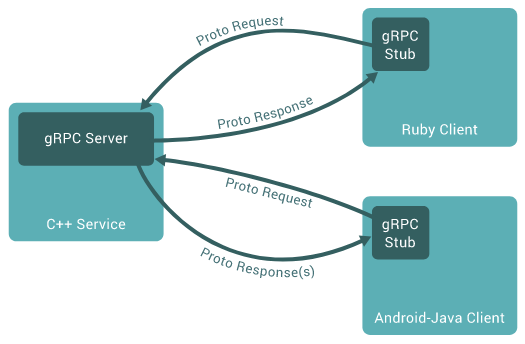
\includegraphics[width=0.8\textwidth]{images/grpc.png}
  \caption[gRPC Framework Structure]{An overview of the structure between client and server in gRPC.}
  \label{fig:gRPC_structure}
\end{figure}\\
\\
\textbf{Protocol Buffers in gRPC}
%hier ein kleiner text
\\
\\
Protocol Buffers are used by default in gRPC and allow structured data to be serialized \cite{Proto}. %With Protocol Buffers, structured data can be specified as message formats. 
The structured data is specified via a message format in the Protocol Buffer file. Afterwards the basic source code of the protocol is automatically generated from the defined message format by executing a Protocol Buffer method. Subsequently, data can be sent from client to server through channels provided by gRPC. Listing \ref{fig:listing3.1} shows the implementation of the protocol header by a Protocol Buffer message format. Each header field is assigned a data type and also a unique field number that determines the order of the fields.\\
%\label{listing4.1} 
\lstinputlisting[language=protobuf2,label=fig:listing3.1 ,style=protobuf,caption={%
The implementation of the DC network protocol header in a Protocol Buffer message format.}]{protobuf/dc_net.proto}
%\label{fig:listing3.1}
%\lstinputlisting[language=protobuf2, style=protobuf,caption={%
%The implementation of the DC network protocol header in a Protocol Buffer %message format.}]{protobuf/dc_net.proto}%\label{listing4.1}
\subsection{Server Implementation}
The server implements all functions that are defined as a service in the Protocol Buffer file. The client implements most of the logic of the DC network. However, when the client accesses a service, most of the service functionality is implemented on the server. Therefore, the client prepares all necessary data and sends the data over a communication channel to the server. The data is then processed by the server and the result is communicated to the client as a response. Listing \ref{fig:listing3.2} shows all service functions implemented on the server. %The data is then processed by the server and the result is communicated to the client as a response. Listing \ref{listing4.2} shows all service functions implemented on the server. 
Each function in the service is defined as an RPC and a name is assigned to the function. In addition, the RPC accepts a message format. For example, the addClientToDCnet function uses the message format defined in Listing \ref{fig:listing3.1}. Afterwards, the functionality of addClienttoDCnet is implemented using gRPC framework.
\\
%\label{listing4.2}
\lstinputlisting[language=protobuf2,label=fig:listing3.2 ,style=protobuf,caption={%
All server functions provided by the DC network service to the client.}]{protobuf/dc_net_server.proto}
%\label{fig:listing3.2}

%\lstinputlisting[language=protobuf2, style=protobuf,caption={%
%All server functions provided by the DC network service to the client.]}{protobuf/dc_net_server.proto}
%\label{listing4.2}
\\ %The functions of the service can be divided into 2 categories. First, helper functions for registration or initialization into the DC network. Second, functions in which logic of the DC net is implemented. In the following, the task of the helper functions is described first. Then the more complex functions are described, which also contain logic of the DC network.
\subsection{Client Implementation}
%hier ein kleiner text
When the in client application starts, a fork function is executed on client-side. The fork function allows a process to create a second process by duplicating the address space of the calling process. The calling process is called parent and the duplicated process is called child. In the application, the parent process takes care of the child process. If the child process crashes, the parent process ensures that the child is restarted correctly. The main logic of the DC network is found in the child process of the client. Only in the child process the services provided by the server are called and used. In addition, the communication channel of gRPC is implemented only on the child. The communication channel forms the interface in which the defined Protocol Buffers can be sent as messages. This means that the parent process has no access to the communication between server and client. Once the communication channel is configured, the interaction between client and server can begin. Figure \ref{fig:Client Implementation} illustrates the structure of the client implementation in a flow chart.
%In the demo, a client is periodically forced to crash so that the error correction procedures can be demonstrated. The actual logic of the application and the communication between client and server is located in the child process. 
\\
\\
\textbf{Initialization}
\\
\\
First, it is assumed that the server is already started. Otherwise, the client cannot be started in gRPC, since no communication channel can be created. The server waits for requests from the client and processes the requests. Second, the child establishes a connection to the electricity provider. In response, the child receives a DC Net identifier and a Client Identifier. A registering client is stored with Client Identifier by the server in a list. This gives the server an overview of the number of participants in the DC Net. In addition, the server can identify faster which client could not send its messages in case of error correction measures. \\
\\
\textbf{Registration}
\\
\\
After a client has received a DC Net Identifier and a Client Identifier, the client requests the server to assign it to a random neighbor. In order for the neighbor and the registering client to synchronize the configuration of their PRNG, both have to perform a Diffie-Hellman key exchange. All the necessary information for calculating the public key is provided by the server and is communicated to the clients on request. In the proposed protocol from the previous chapter, it was described that the electricity provider must offer a tunnel so that two \gls{SMGW}s can communicate and exchange public keys via Diffie-Hellman with each other. The tunnel in the protocol represents the communication channel in gRPC. But in gRPC all RPC requests are started by the client. The server only responds to the client's requests. Forwarding messages from a requesting clients to a non-requesting clients is therefore not possible or very difficult to implement in gRPC. Instead of the public keys being forwarded to the clients by the server, as suggested in the protocol, the public keys are stored by the clients on the server for a short time and the clients make a request for the public keys. 
Each client only needs to obtain the public key of its neighbor through a request to the server and is able to compute the secret key. After the Diffie-Hellman key exchange has been executed and the PRNG has been configured, the client can create the local superposition and send its local superposition to the server for each round. 
\\
\\
\textbf{Generation of the global Superposition}
\\
\\
The server receives all the local superposition and adds them up to get the global superposition. Subsequently, the server verifies the correctness of the global superposition. If the global superposition is incorrect, then a client in a DC network has failed and could not send a local superposition. The defective client is located by the server by looking up which client has not sent a local superposition to the server. Afterwards the neighboring clients are instructed by the server to recalculate the local superposition without using the key of the failed client and resent it to the server. The global superposition is then updated by the power provider. \\
\\
\textbf{Preparations for the next Round}
\\
\\
After each sending of the local superposition, all clients check whether a new subscriber wants to register in the DC network. If so, one client is notified by the server that it gets a new neighbor. Subsequently, another registration process takes place with the Diffie-Hellman key exchange which was described before. Another deviation from the protocol is that in the implementation each client has no minimum number of neighbors than the required 3 neighbors in the protocol. The flow chart in Figure \ref{fig:Client Implementation} illustrates the structure of the client implementation with the key functions.
\begin{figure}[tbp]
  \centering
  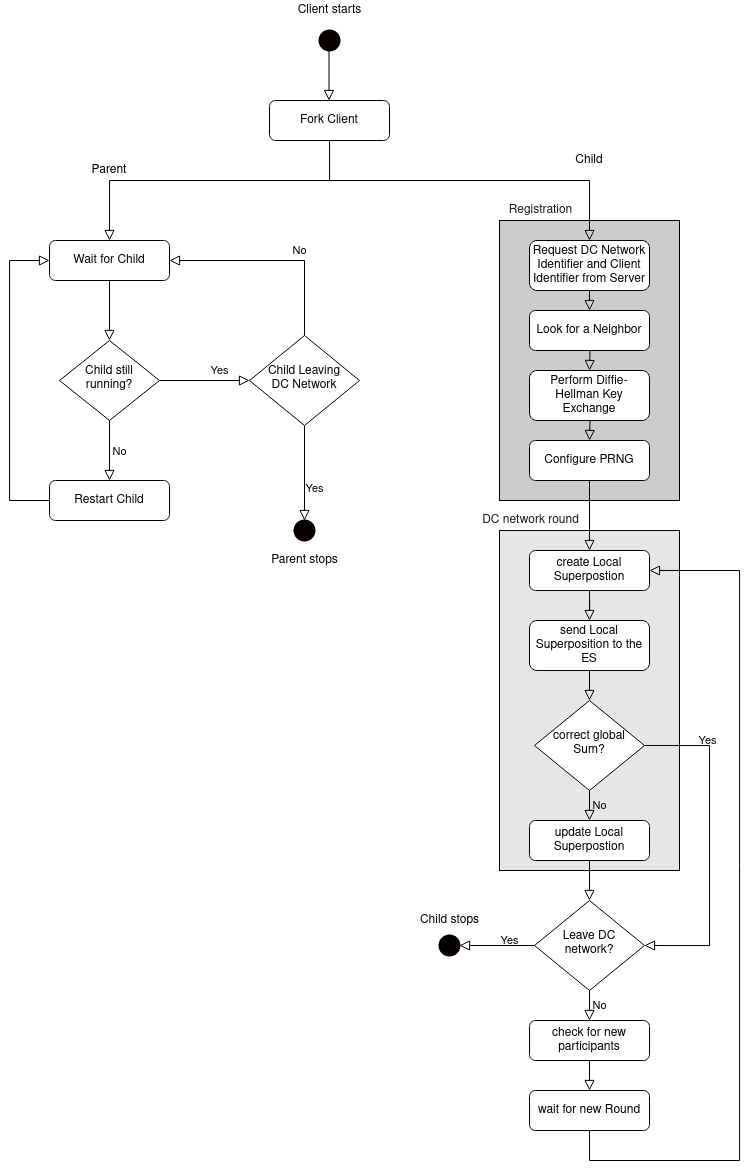
\includegraphics[width=0.8\textwidth]{images/Client_structure.png}
  \caption[Flowchart Client Implementatioen]{The flowchart shows all program operations that are performed in the client.}
  \label{fig:Client Implementation}
\end{figure}

%\\
%\textbf{Helper Functions}
%%\\
%\\
%The helper functions in the service mainly perform tasks to register the client in the DC network or to ensure client communication with each other. Therefore, the helper functions do not take over any core logic in the DC network. In the following a documentation with the tasks of the functions is described.
%\begin{enumerate}
%\item addClientToDCnet:\\
%The first action that the client child performs is to register on the DC network. For this the addClientToDCnet function is used. In the server the request from the client is processed. The client is assigned a client identifier and the identifier is added to a list so that the service has an overview of all clients in the DC network.
%\item ConnectDCClients:\\
%The ConnectDCClients function assigns a random neighbor to a requesting client.

%\end{enumerate}
%\\
%\\
%\textbf{DC Network Functions}
%\\
%\\

\subsection{Challenges}
Several challenges were encountered during the implementation in this thesis. The most serious and time-consuming 2 errors are described below.\\
\\
\textbf{Multiple Client access on the Server}
\\
\\ 
In the experimental environment, three clients communicate with a server. A particular challenge was therefore to implement the server cleanly and consistently so that multiple clients could access the same function or even the same line of code at the same time without the server crashing or the program entering an inconsistent state. The implementation was thus particularly difficult in the service functions in which the calculations of the global superposition or the verification of the global superposition were carried out.%vllt noch irgendwas schreiben mit Da der Author zuvor noch keine Erfahrung in verteilen Programmieren hatte etc.
\\
\\
\textbf{gRPC Client-to-Client Communication}
\\
\\
The protocol defined that the electricity provider must provide a tunnel for \gls{SMGW} to \gls{SMGW} communication. It was tried to implement the same structure as in the protocol. However, the clients in the gRPC framework do not receive an \gls{IP} address, so the server cannot distinguish calls from different clients. In search of a solution the following suggestions have been considered. 
\begin{enumerate}
\item Setup a Server on each Client:\\
In this approach, each Raspberry Pi on which a client application is implemented would get an additional server that can communicate with the power provider. In addition, a client would have to be implemented on the power provider so that requests from the power provider can be sent to clients over a communication channel. In the work it was decided against it, because it is a considerable additional effort and requires an extra implementation of servers on the clients.
\item Bi-directional Streaming:\\
gRPC offers different ways to send messages. One way is a bidirectional streaming RPC where server and client exchange a sequence of messages via a stream. In gRPC can be configured depending on the use.
For example in a message stream the server can wait for all client requests before responding or it can respond immediately after each message. It can be defined in the Protocol Buffer syntax with the keyword stream. The stream property can be exploited to implement message forwarding in gRPC. Various solution sketches have been found that promote this approach. However, the proposed solutions were vague and storing the public keys in the short term on the server was much simpler to implement. 
\end{enumerate}\\
%\\
%\textbf{Crashing Parent}
%\\
%\\
%During the implementation there were indeterministic crashes of the parent in the client. The error could not be traced for a long time, because the crash occurred at different times during the runtime of the application. When the parent crashes, the child continues to work without interruptions. However, the child cannot be restarted if the parent crashes. It has been found by accident that the fork function is not executed correctly after the communication channel has been created.  
%sowas schreiben wie, dass der Mehrfachzugriff auf den Server problematisch war und schwer zu implementieren, da du noch nie mit verteilten Systemen gearbeitet hast. Dann noch schreiben, dass grpc die technischen mögichkeiten eingeschränkt hat, da es keine Client zu CLient kommunikation gab. Vllt zusammenfassen, dass die Clients einfach zu implementieren waren, aber die schwerste aufgabe der server war. Das Problem mit dem Kommunikationskanal und das der Parent die ganze zeit abgestürzt ist.

%Den Service noch beschreiben!


\section{Evaluation}
\label{Evaluation}
In this chapter the properties of the DC network are analyzed. Various characteristics are evaluated, including the performance of the process, the security and the necessary minimum size of the network.
\subsection{Performance}
\label{performance}
Regarding the performance, it is considered to what extent the proposed network is more efficient or inefficient compared to the \gls{TR-03109}. In addition, the message and memory volume generated by the protocol is considered.
\\
\\
\textbf{Computational Performance}
\\
\\
The proposed DC network is highly scalable. Due to the fact that on the \gls{SMGW} side only a simple computation of the power consumption with a generated key through a PRNG has to be performed to form the local superposition, hardly any computational power will have to be used. Furthermore, a local superposition is sent only every 15 minutes. The computational overhead caused by the sending the local superposition is negligible for the \gls{SMGW} and the protocol should be able to run without problems even on lightweight systems. It has to be considered that the used PRNG really generates random numbers. The built-in hardware security module in the \gls{SMGW} offers cryptographically secure PRNG. On the side of the power provider, only simple operations need to be performed as well. Every single received local superposition of a \gls{SMGW} has to be added up to form the global superposition. Addition of many thousands of summands is no problem for ordinary computers and the complexity of the calculation does not deviate from the proposal of the \gls{TR-03109}, since the transmitted data has to be summed up as well.\\
In case of the error correction the transmission bit allows the power provider to immediately detect which \gls{SMGW} in the network has failed. Even if several \gls{SMGW} fail at the same time, it is no issue for the neighboring \gls{SMGW} to resend the updated local superposition to the power provider. Afterwards, the electricity provider efficiently calculates the global superposition \ref{error_corr_conn}.\\
\\
\textbf{Message Overhead}
\\
\\
The messages sent in the protocol can be implemented with a small header. The message field in which the local superposition are entered must always be the same size, otherwise the DC network cannot be implemented. Therefore, large data packets are not to be expected, since the local superposition require a sufficiently large message field, which will not require more than several 100 bytes. \\
\\
\textbf{Message Volume}
\\
\\
When registering a requesting \gls{SMGW} in a DC network, several messages must be exchanged between the \gls{SMGW} and the electricity provider as well as between the requesting \gls{SMGW} and the neighbor \gls{SMGW}. If a DC network round runs without errors, no additional messages are exchanged.
%In case of error correction measures, a large number of multiple messages must be sent, otherwise no meaningful global sum can be calculated and the members in a DC network must coordinate to correct the error. Considering that normally only one message is sent to the power provider every 15 minutes, it should be bearable for the power provider if there is a minimal to medium traffic volume every 15 minutes in a DC network.
However, an increased message volume is to be expected during error correction. Especially in the case of an active attacker, several phases will be run in F-mode, requiring message exchange between client and server. However, it must be mentioned that most of the time in the DC network no messages are exchanged at all. Messages are only transmitted when a client enters or leaves, or when the local superposition is sent. If the local superposition fails, the system has enough time to correct the error until the next round. Therefore, an increased message volume due to the error correction can be tolerated.\\
\\
\textbf{Memory Overhead}
\\
\\
The memory overhead of \gls{SMGW} in a DC network is minimal. Only the PRNG key from the neighbors need to be stored. However, the power provider needs to store the key graph. For this reason the power provider has a larger storage overhead compared to the \gls{TR-03109}. Additionally, it must be assumed that the electricity provider will operate multiple DC networks simultaneously. Therefore, a medium storage overhead is expected.

\subsection{Security}
The security evaluation considers the extent to which the security objectives are better or worse protected compared to the \gls{TR-03109} from the \gls{BSI}. Possible attacks on the security objectives have already been explained in the Design chapter \ref{error_corr} and in the related work chapter \ref{subsec:attacks}.
\\
\\
\textbf{Availability}
\\
\\
Availability is one of the most important security objectives of the DC network. If an \gls{SMGW} should fail, e.g. due to a missing Internet connection, then no global superposition can be formed and the functionality of the network is not possible. This is equivalent to an unavailable network for the power provider. Measures have been described to deal with this failure. If an attacker succeeds in taking over an \gls{SMGW}, he can deliberately send incorrect local superposition with the intention of disrupting availability. Against this active attack, an algorithm was proposed that allows the power provider to switch to F-mode and search for the attacker and restore availability. According to this, temporary outages may occur in the DC network, but all of them can be solved in a short time by troubleshooting procedures. A degradation of availability is therefore not expected.
\\
\\
\textbf{Anonymity}
\\
\\
By using PRNGs, anonymity decreases from information-theoretically secure to complexity-theoretically secure anonymity. Nevertheless even if an \gls{SMGW} is controlled by an attacker, it would not be possible for the attacker to read the power consumption of other \gls{SMGW}s. This is because the attacker has no access to the global superposition. This can only be calculated by the electricity provider. With the proposed method, the attacker lacks the necessary information to launch a potential attack on the DC network\footnote[4]{Assuming the attacker does not have control over a large number of \gls{SMGW} in the DC network.}. Furthermore, the attacker also has no information about the key graph. This further complicates the chances of a successful attack and to deanonymize the electricity consumption of costumers. The electricity provider is potentially the most dangerous attacker in the protocol, since the \gls{SMGW}s cannot communicate with each other, they rely on the electricity provider to register in the DC network. As a result, the power provider has to take over administrative tasks and therefore possesses a lot of control. To ensure that the electricity supplier is not too powerful, its competences have been restricted. The best chance of the electricity provider to break the anonymity to its customers is that the administrative powers are abused to connect individual \gls{SMGW}s to malicious neighbors. Once the electricity provider manages to link an \gls{SMGW} with only malicious neighbors, the local superposition can be reconstructed and the electricity consumption is visible. This is prevented by forcing the electricity provider to select a random neighbor in the registering phase for a registering \gls{SMGW}. Additionally, the electricity provider should be technically forced, that it can't remove a random \gls{SMGW} at will, but only if an \gls{SMGW} wants to leave the DC network by itself. These measures make it almost impossible for the electricity provider to affect the selection of neighbors in the DC network.
\\
\\
\textbf{Eavesdropping}
\\
\\
In the case of eavesdropping on one or more channels of \gls{SMGW}s by an attacker, attackers can read but not understand payload data because the local superposition is not a meaningful message. An attacker can therefore only observe when an \gls{SMGW} sends local superposition. Furthermore, the attacker can assume from an increased message volume that an error correction procedure is being used in the DC network. 
\\
\\
\textbf{Malicious Electricity Provider}
\\
\\
The strongest attacker in the DC network is an electricity provider that has malicious intent with the motivation to obtain additional privacy compromising data. Due to the advanced administrative functions available to the electricity provider, the electricity provider could be tricked into exploiting its administrative rights. Therefore, there is a fine line between granting administrative privileges to the electricity provider to maintain the DC network and restricting administrative privileges so that the electricity provider cannot breach security. Careful consideration has been given in the design to what powers are necessary for the electricity provider. However, if a malicious power provider does tamper with the DC network, the \gls{SMGW} will have the ability to leave the DC network.
\\
\\
\textbf{Protocol compatibility with the TR-03109}
\\
\\
The protocol has been designed with the structural specifications of the \gls{TR-03109}. Therefore, after implementation, it could be integrated into the currently specified German smart grid without any major complications. The \gls{WAN} interface of the \gls{SMGW} does not need to be extended and existing communication links are not affected by the protocol. 
But the biggest weakness in the presented protocol is the electricity provider, since it knows the key graph. This design decision was made only because the technical policy does not allow direct communication between two \gls{SMGW}s via the \gls{WAN} interface. If this requirement were changed in the \gls{TR-03109}, then a decentralized DC network could be integrated into the German smart grid. This would make attacks from a malicious electricity provider impractical.

\clearpage

%%% Local Variables:
%%% TeX-master: "diplom"
%%% End:

%%% Local Variables:
%%% TeX-master: "diplom"
%%% End:



%%% Local Variables:
%%% TeX-master: "diplom"
%%% End:


\chapter{}
\label{sec:Appendix}
% Hier greift man einige wenige, interessante Gesichtspunkte der
% Implementierung heraus. Das Kapitel darf nicht mit Dokumentation oder
% gar Programmkommentaren verwechselt werden. Es kann vorkommen, daß
% sehr viele Gesichtspunkte aufgegriffen werden müssen, ist aber nicht
% sehr häufig. Zweck dieses Kapitels ist einerseits, glaubhaft zu
% machen, daß man es bei der Arbeit nicht mit einem "Papiertiger"
% sondern einem real existierenden System zu tun hat. Es ist sicherlich
% auch ein sehr wichtiger Text für jemanden, der die Arbeit später
% fortsetzt. Der dritte Gesichtspunkt dabei ist, einem Leser einen etwas
% tieferen Einblick in die Technik zu geben, mit der man sich hier
% beschäftigt. Schöne Bespiele sind "War Stories", also Dinge mit denen
% man besonders zu kämpfen hatte, oder eine konkrete, beispielhafte
% Verfeinerung einer der in Kapitel 3 vorgestellten Ideen. Auch hier
% gilt, mehr als 20 Seiten liest keiner, aber das ist hierbei nicht so
% schlimm, weil man die Lektüre ja einfach abbrechen kann, ohne den
% Faden zu verlieren. Vollständige Quellprogramme haben in einer Arbeit
% nichts zu suchen, auch nicht im Anhang, sondern gehören auf Rechner,
% auf denen man sie sich ansehen kann.
\begin{figure}[H]
  \centering
  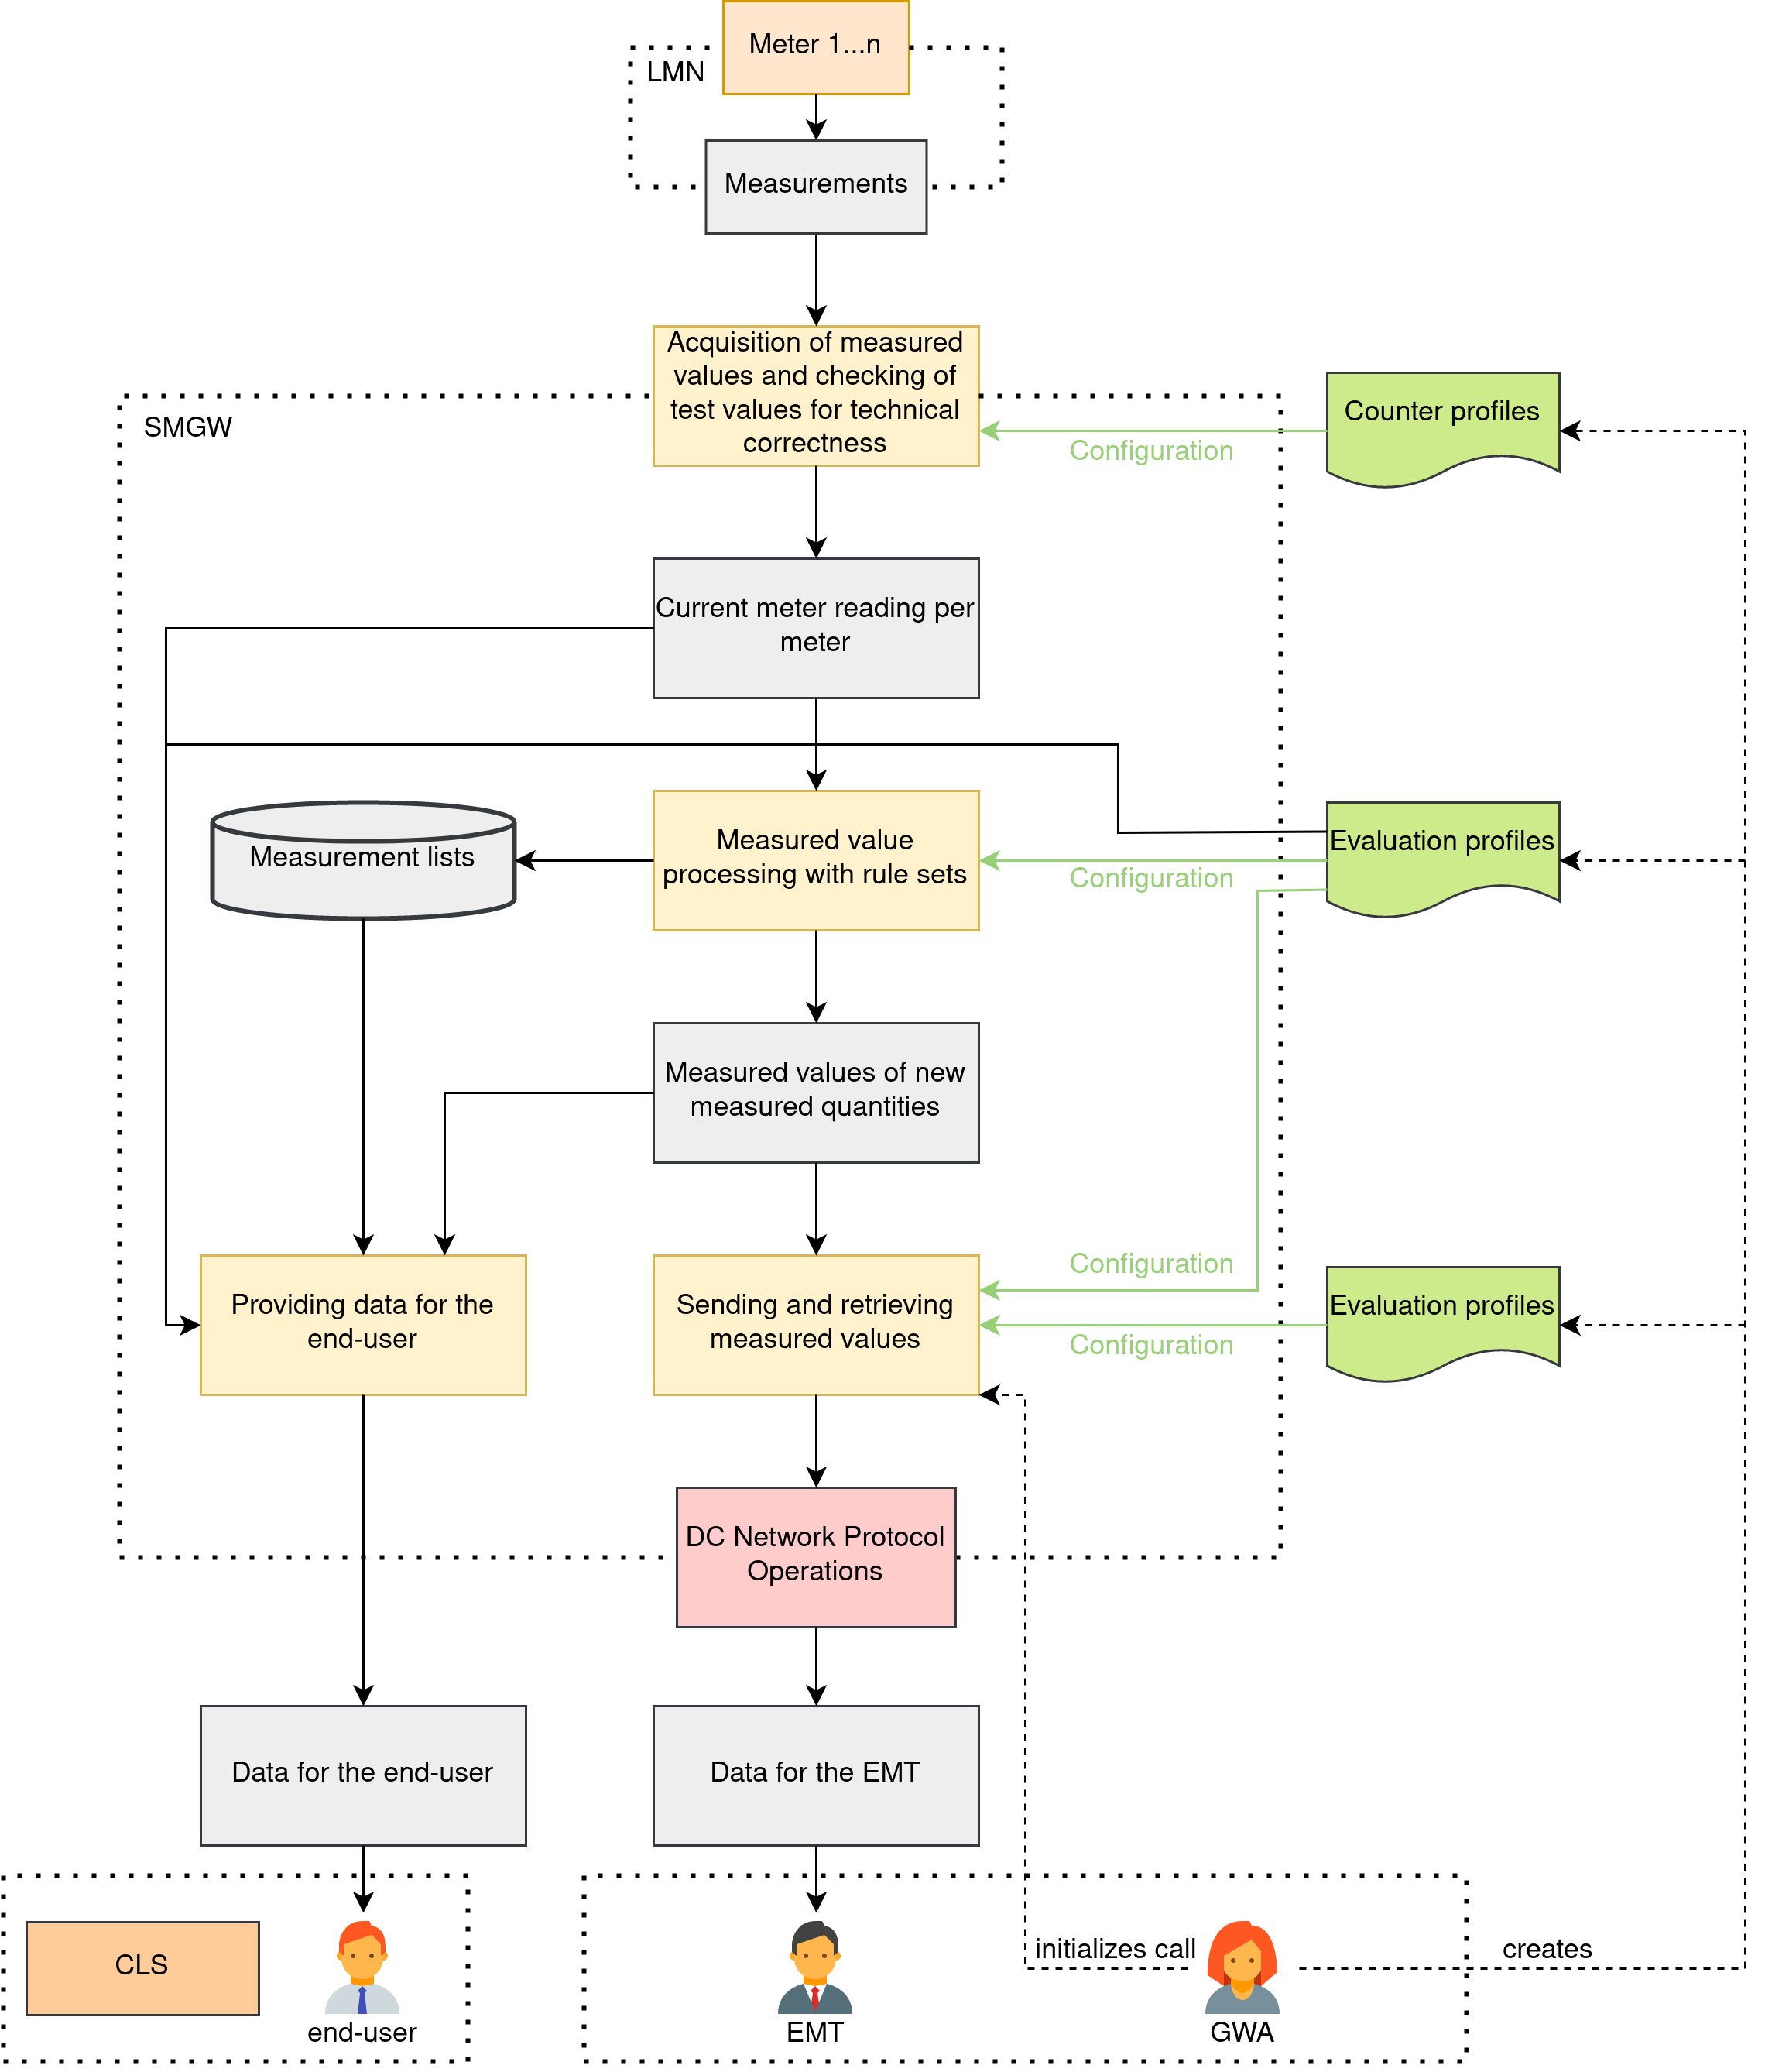
\includegraphics[width=1\textwidth]{images/Messverarbeitung_mit_DC_Eng2.png}
  \caption[Measured Value Processing in a SMGW]{An overview of the measured value processing within the SMGW with configuration profiles from the GWA and DC Network Protocol Extension.}
  \label{fig:value_processing_with_dc}
\end{figure}
%\renewcommand\topfraction{1}   
%\renewcommand\floatpagefraction{1}
\chapter{Two Weeks Experiments}
\enlargethispage{10}
\vspace*{-10\baseline}
\begin{figure}[!Hhtp]
\centering
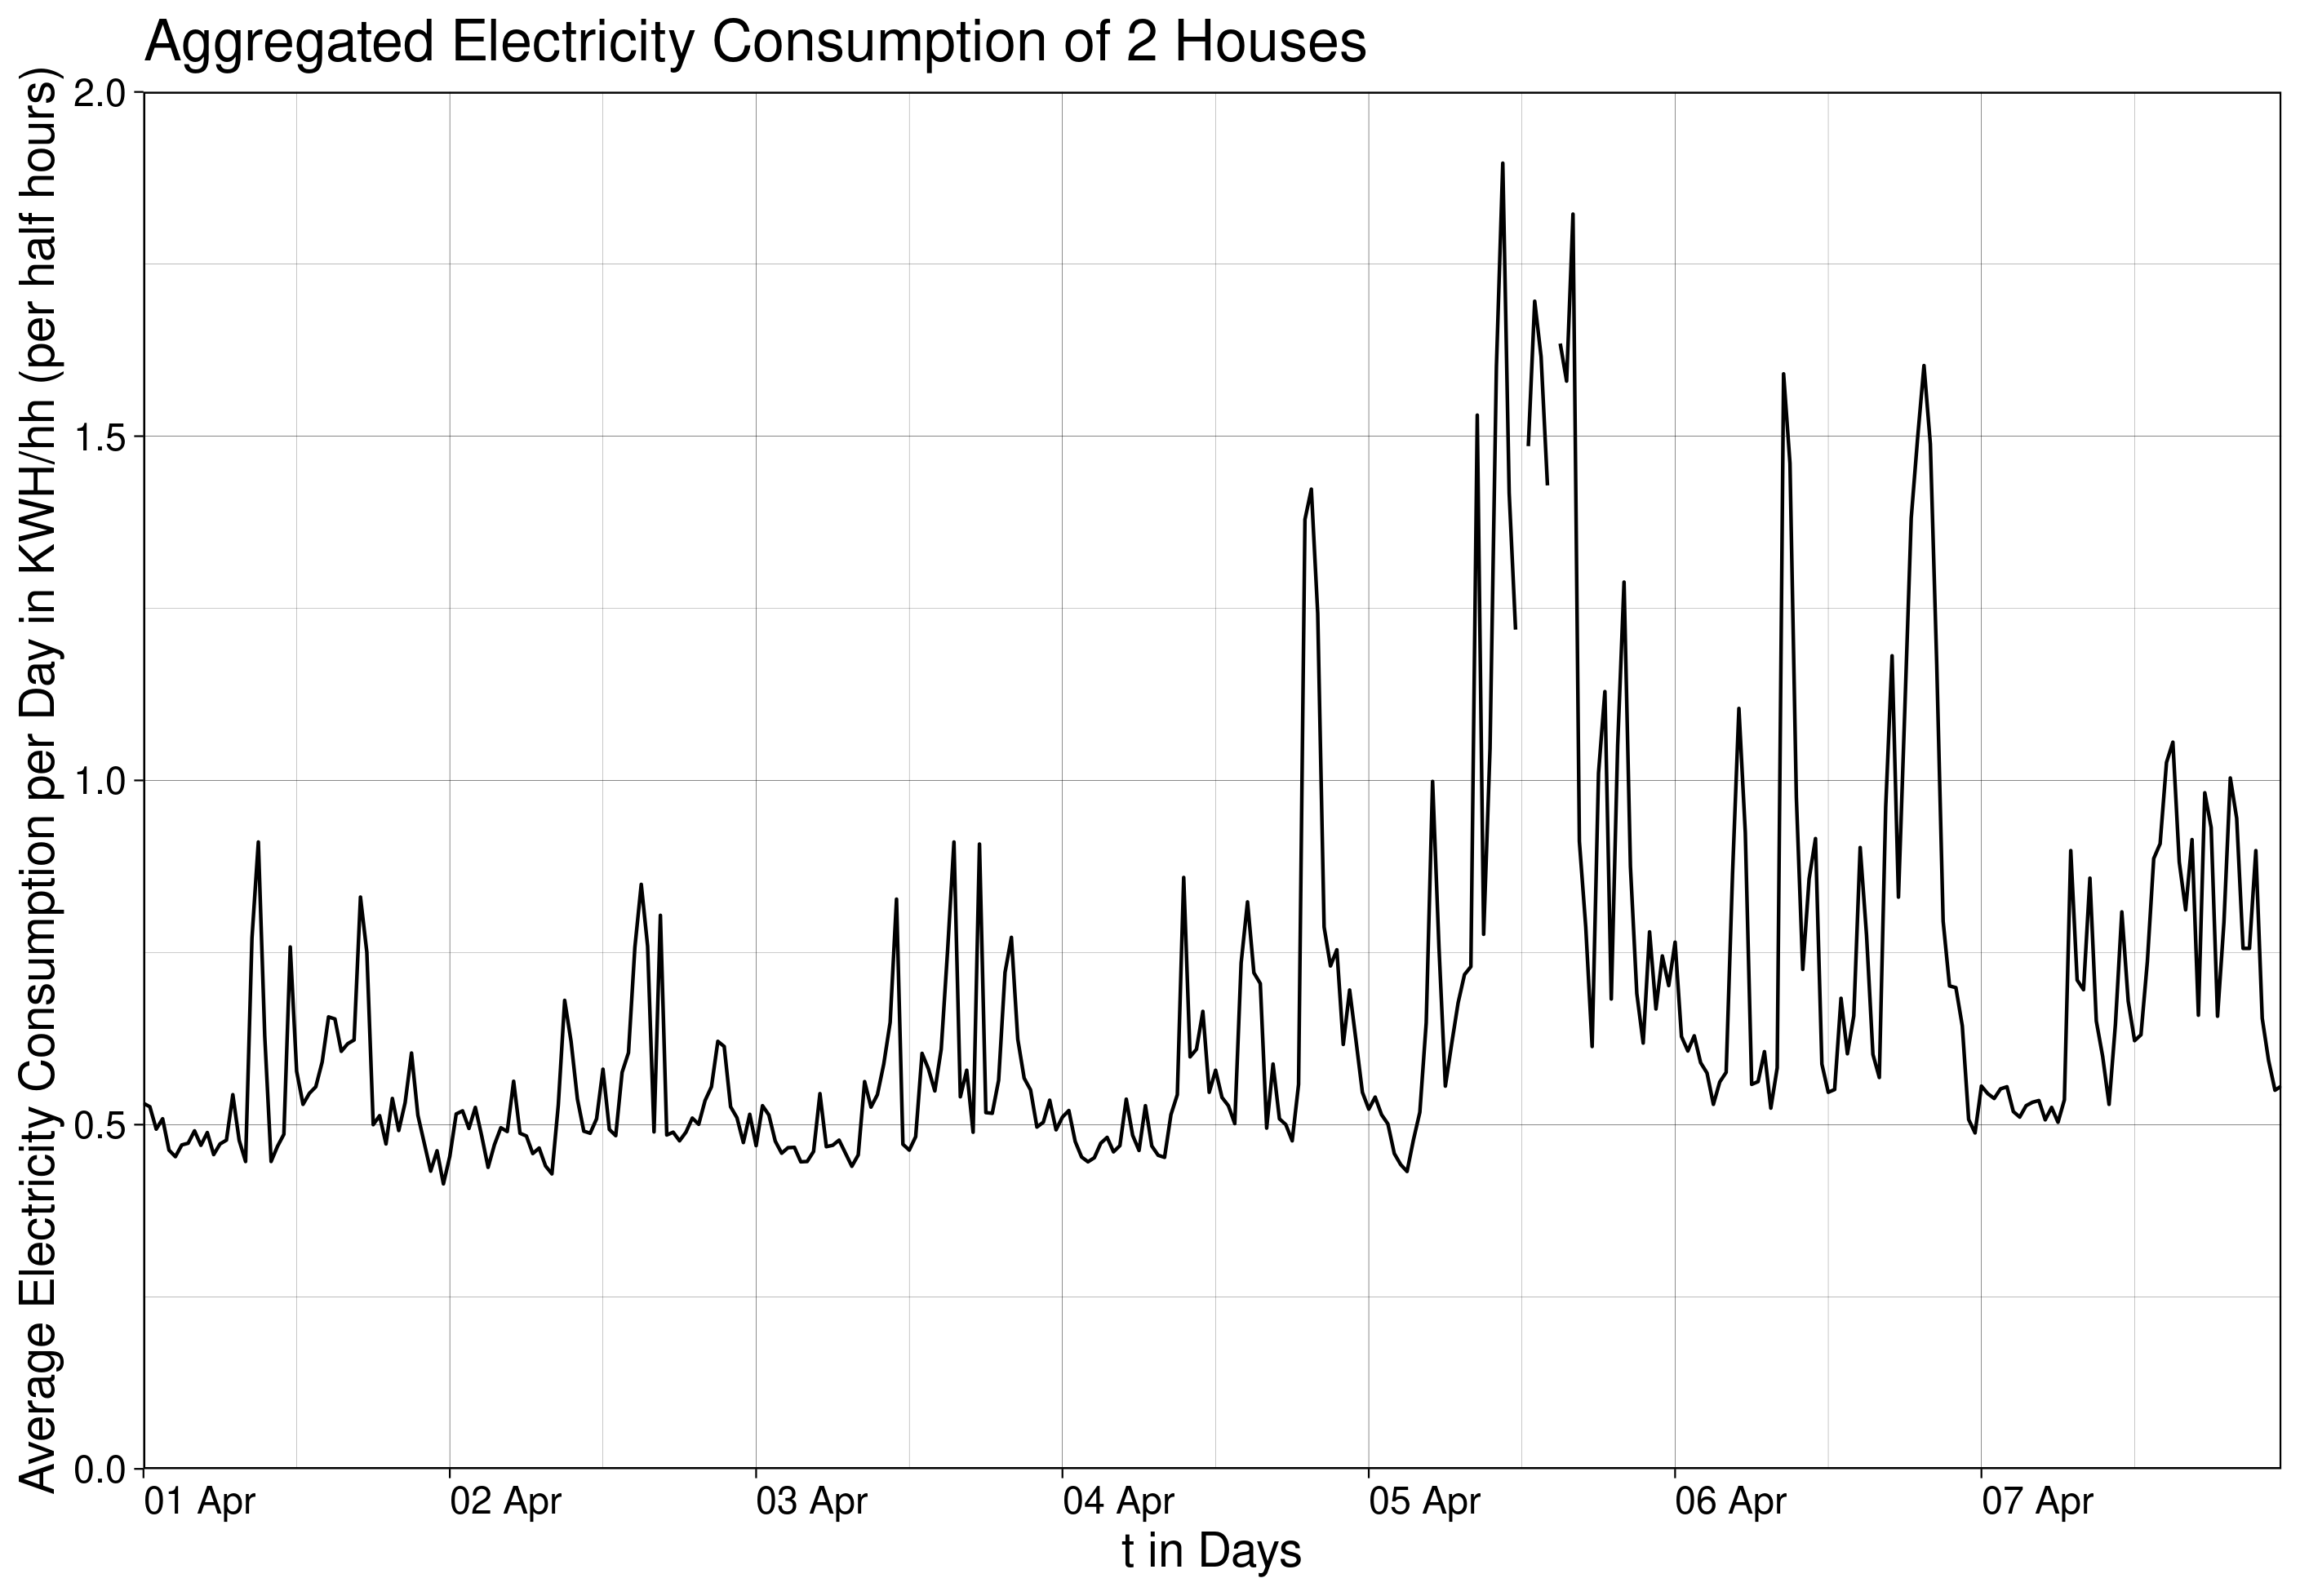
\includegraphics[width=0.8\columnwidth]{images/Aggregated Electricity Consumption of 2 Houses6.png}
\caption[Aggregated Electricity Consumption of 2 Houses of the 2nd Experiment of the 2nd Experiment]{}
\label{img:2_Houses_weekly}
%\vspace*{\floatsep}
\centering
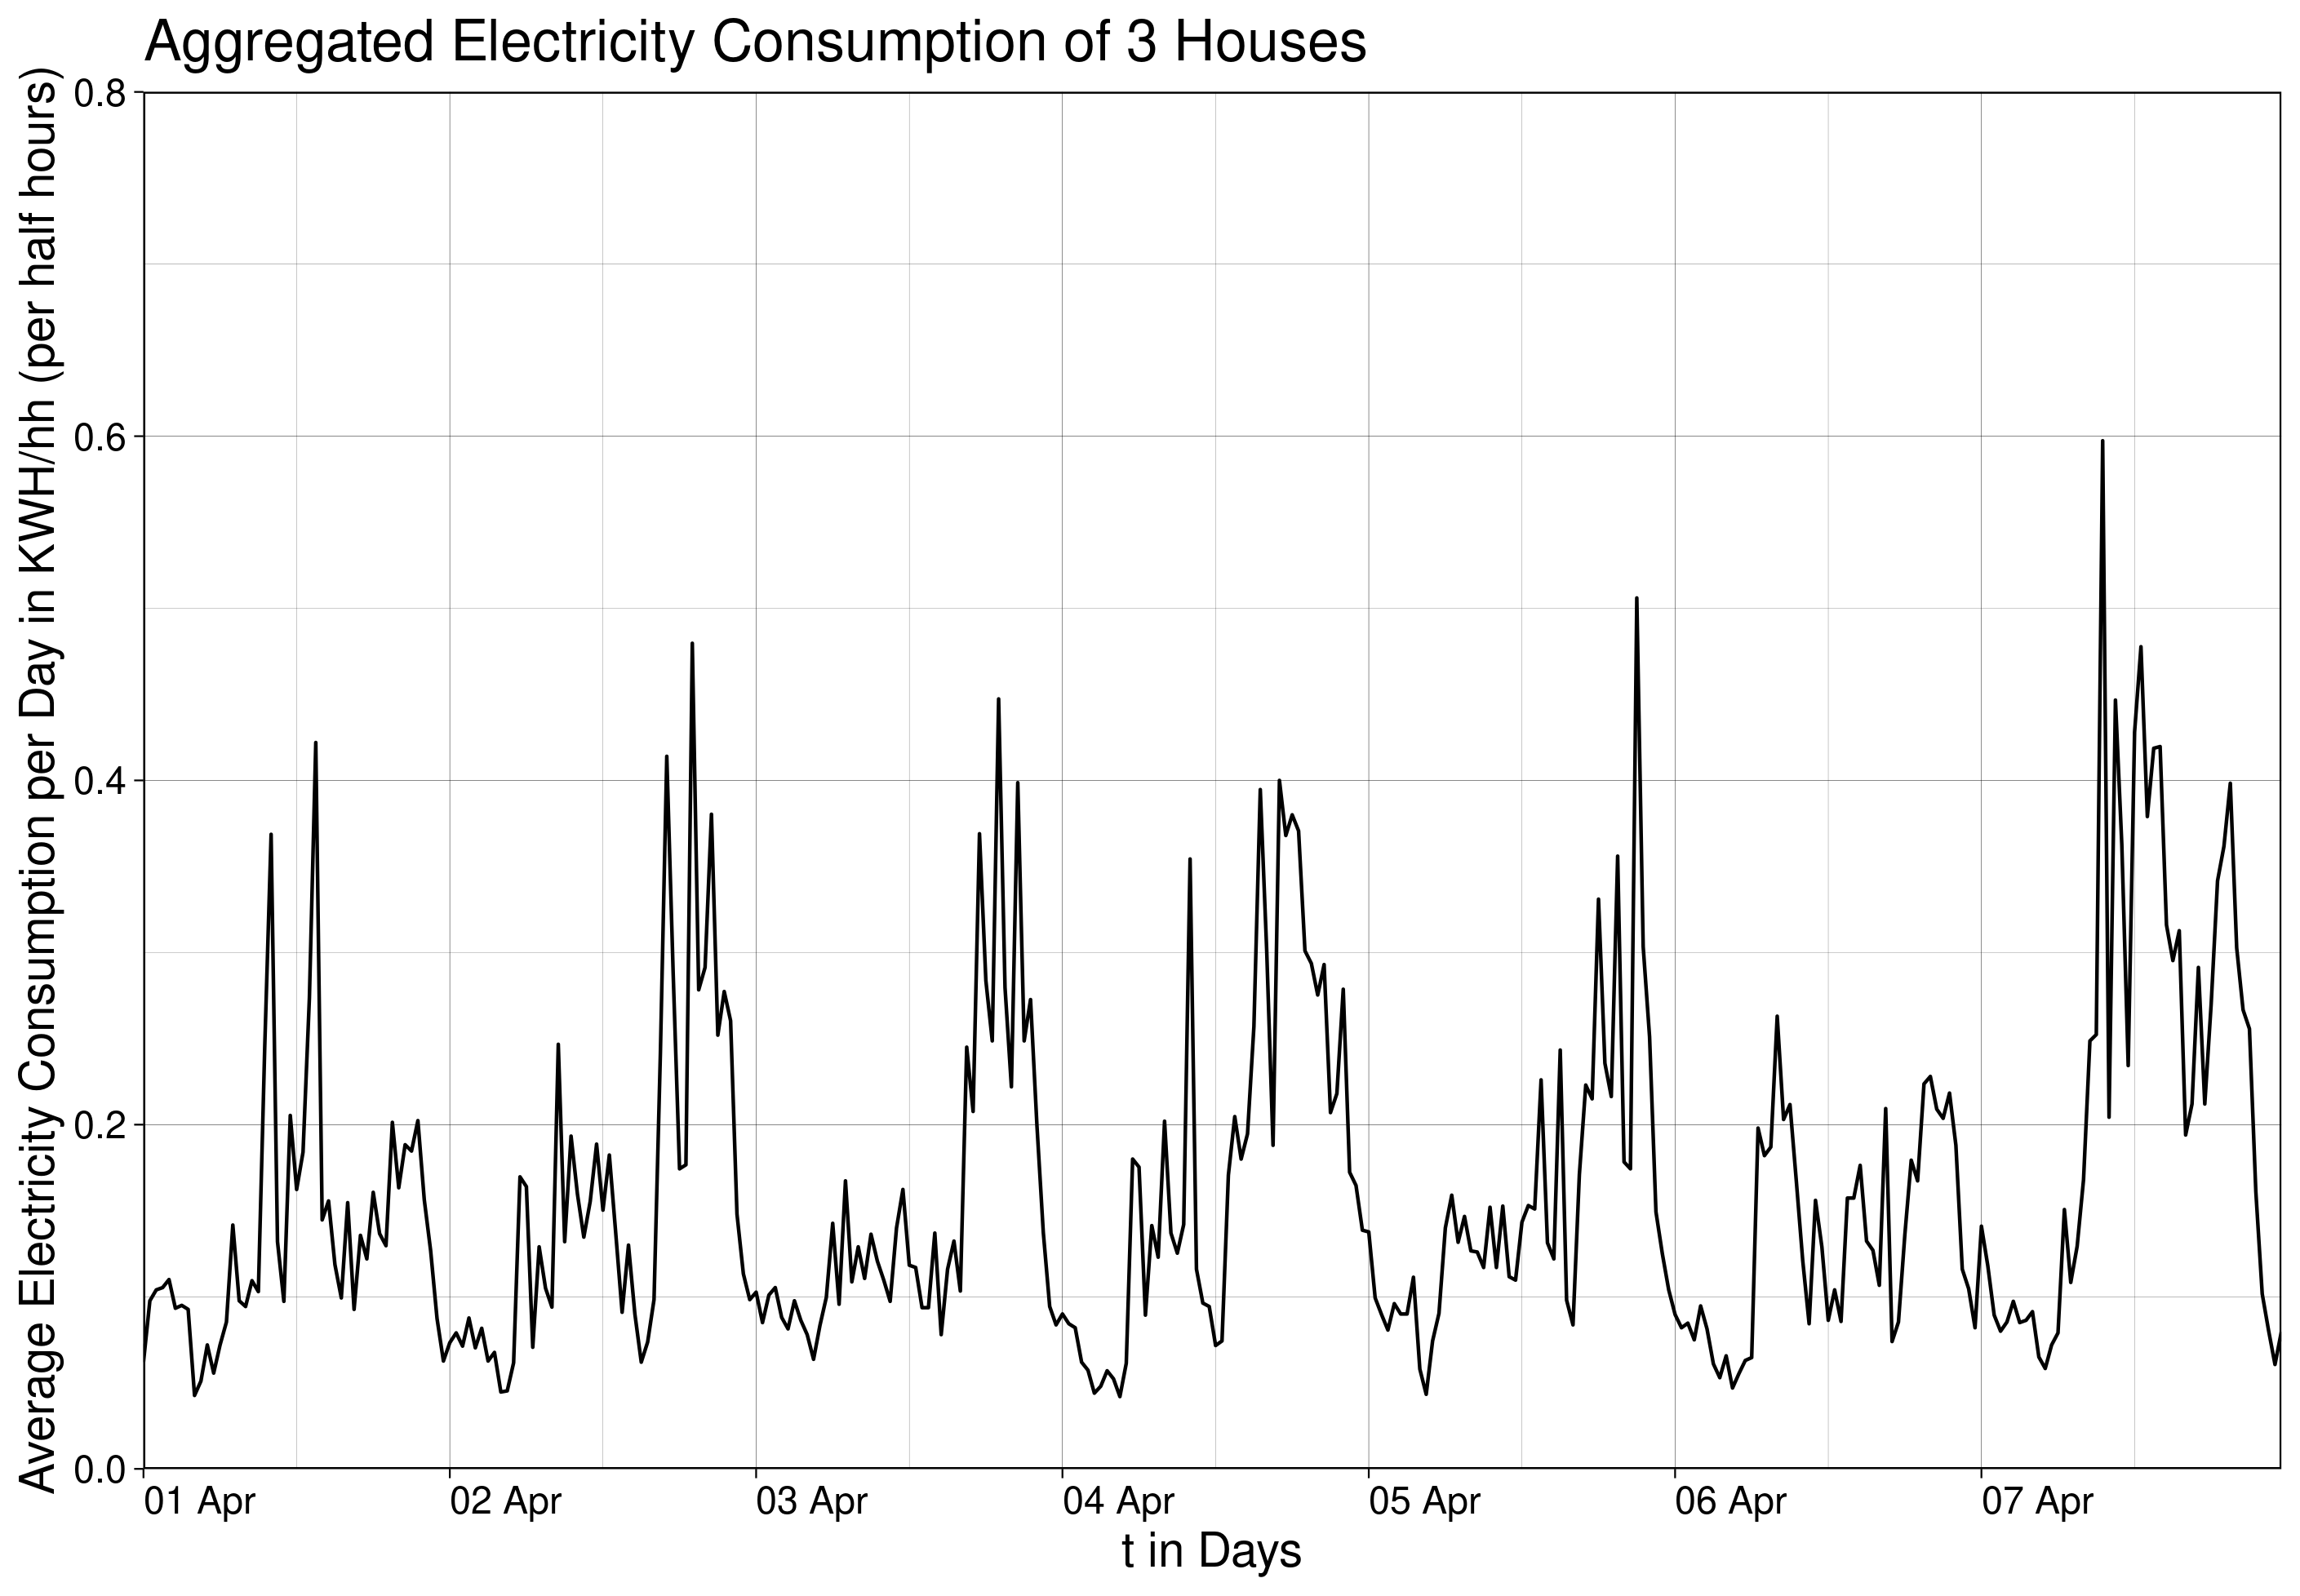
\includegraphics[width=0.8\columnwidth]{images/Aggregated Electricity Consumption of 3 Houses5.png}
\caption[Aggregated Electricity Consumption of 3 Houses of the 2nd Experiment]{}
\label{img:3_Houses_weekly}
\end{figure}

\nopagebreak
\afterpage{%
\begin{figure}[!p]
\centering
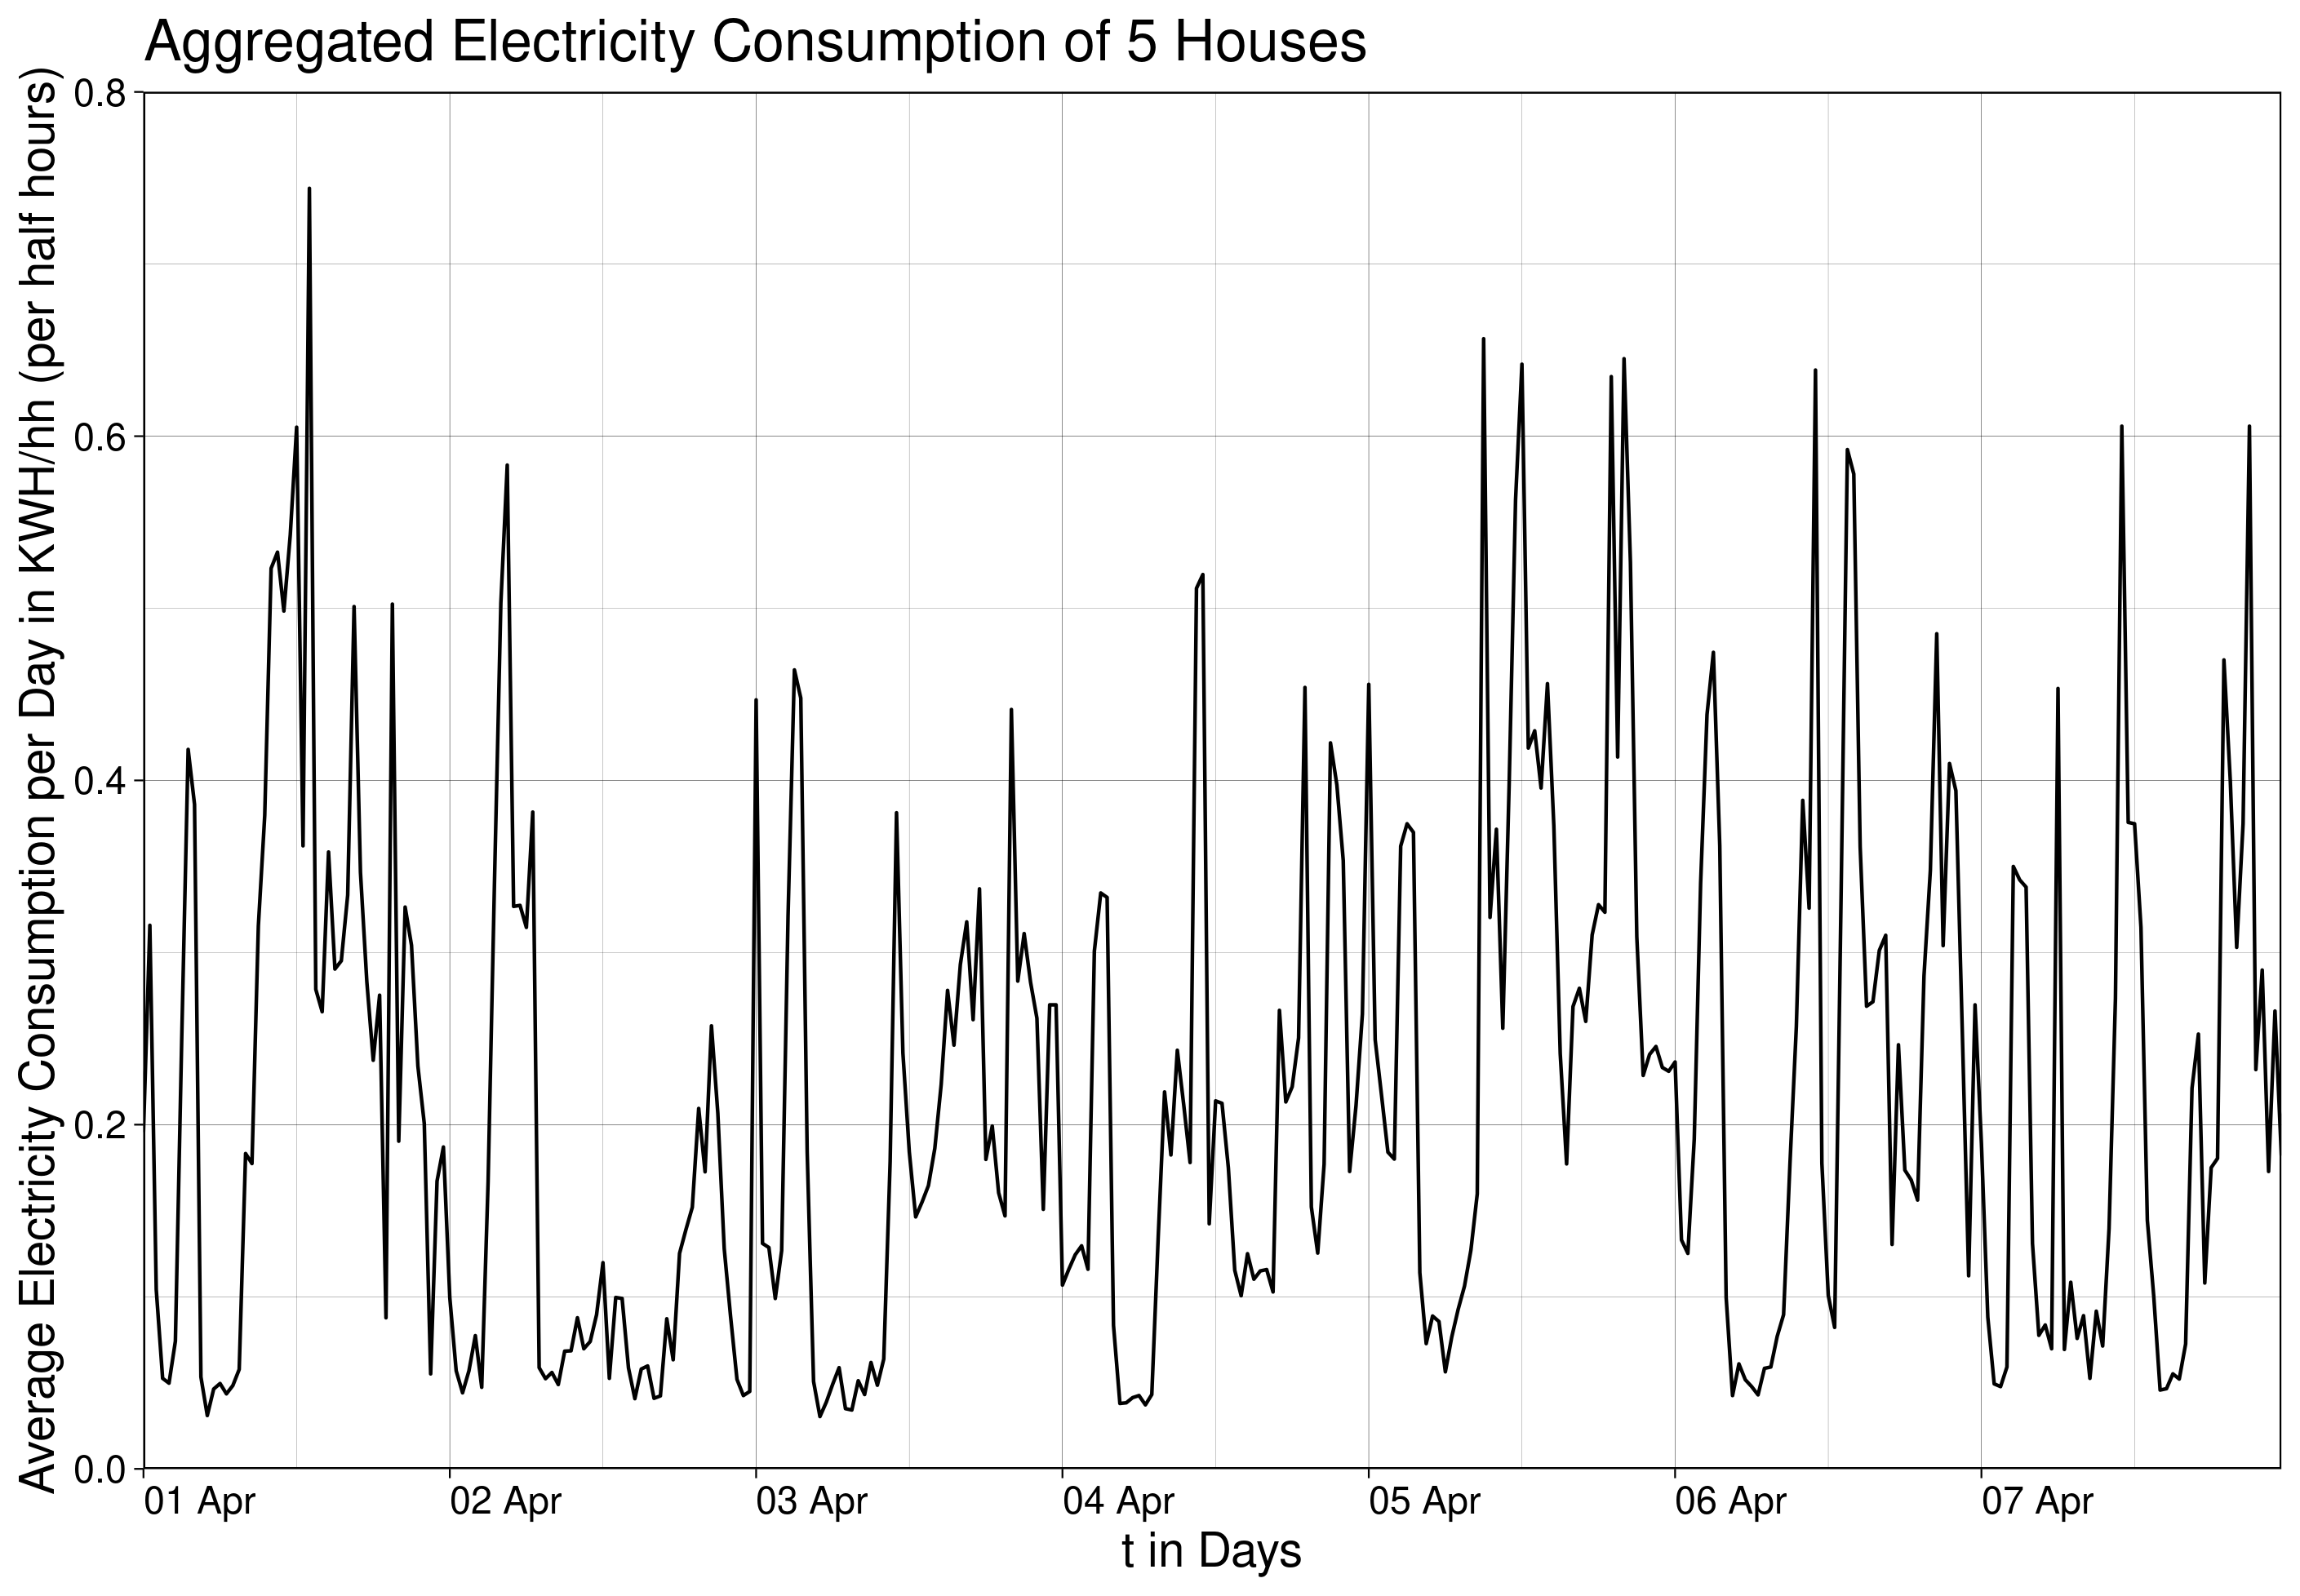
\includegraphics[width=0.85\textwidth]{images/Aggregated Electricity Consumption of 5 Houses5.png}
\caption[Aggregated Electricity Consumption of 5 Houses of the 2nd Experiment]{}
\label{img:5_Houses_weekly}
\end{figure}
\begin{figure}[!p]
\centering
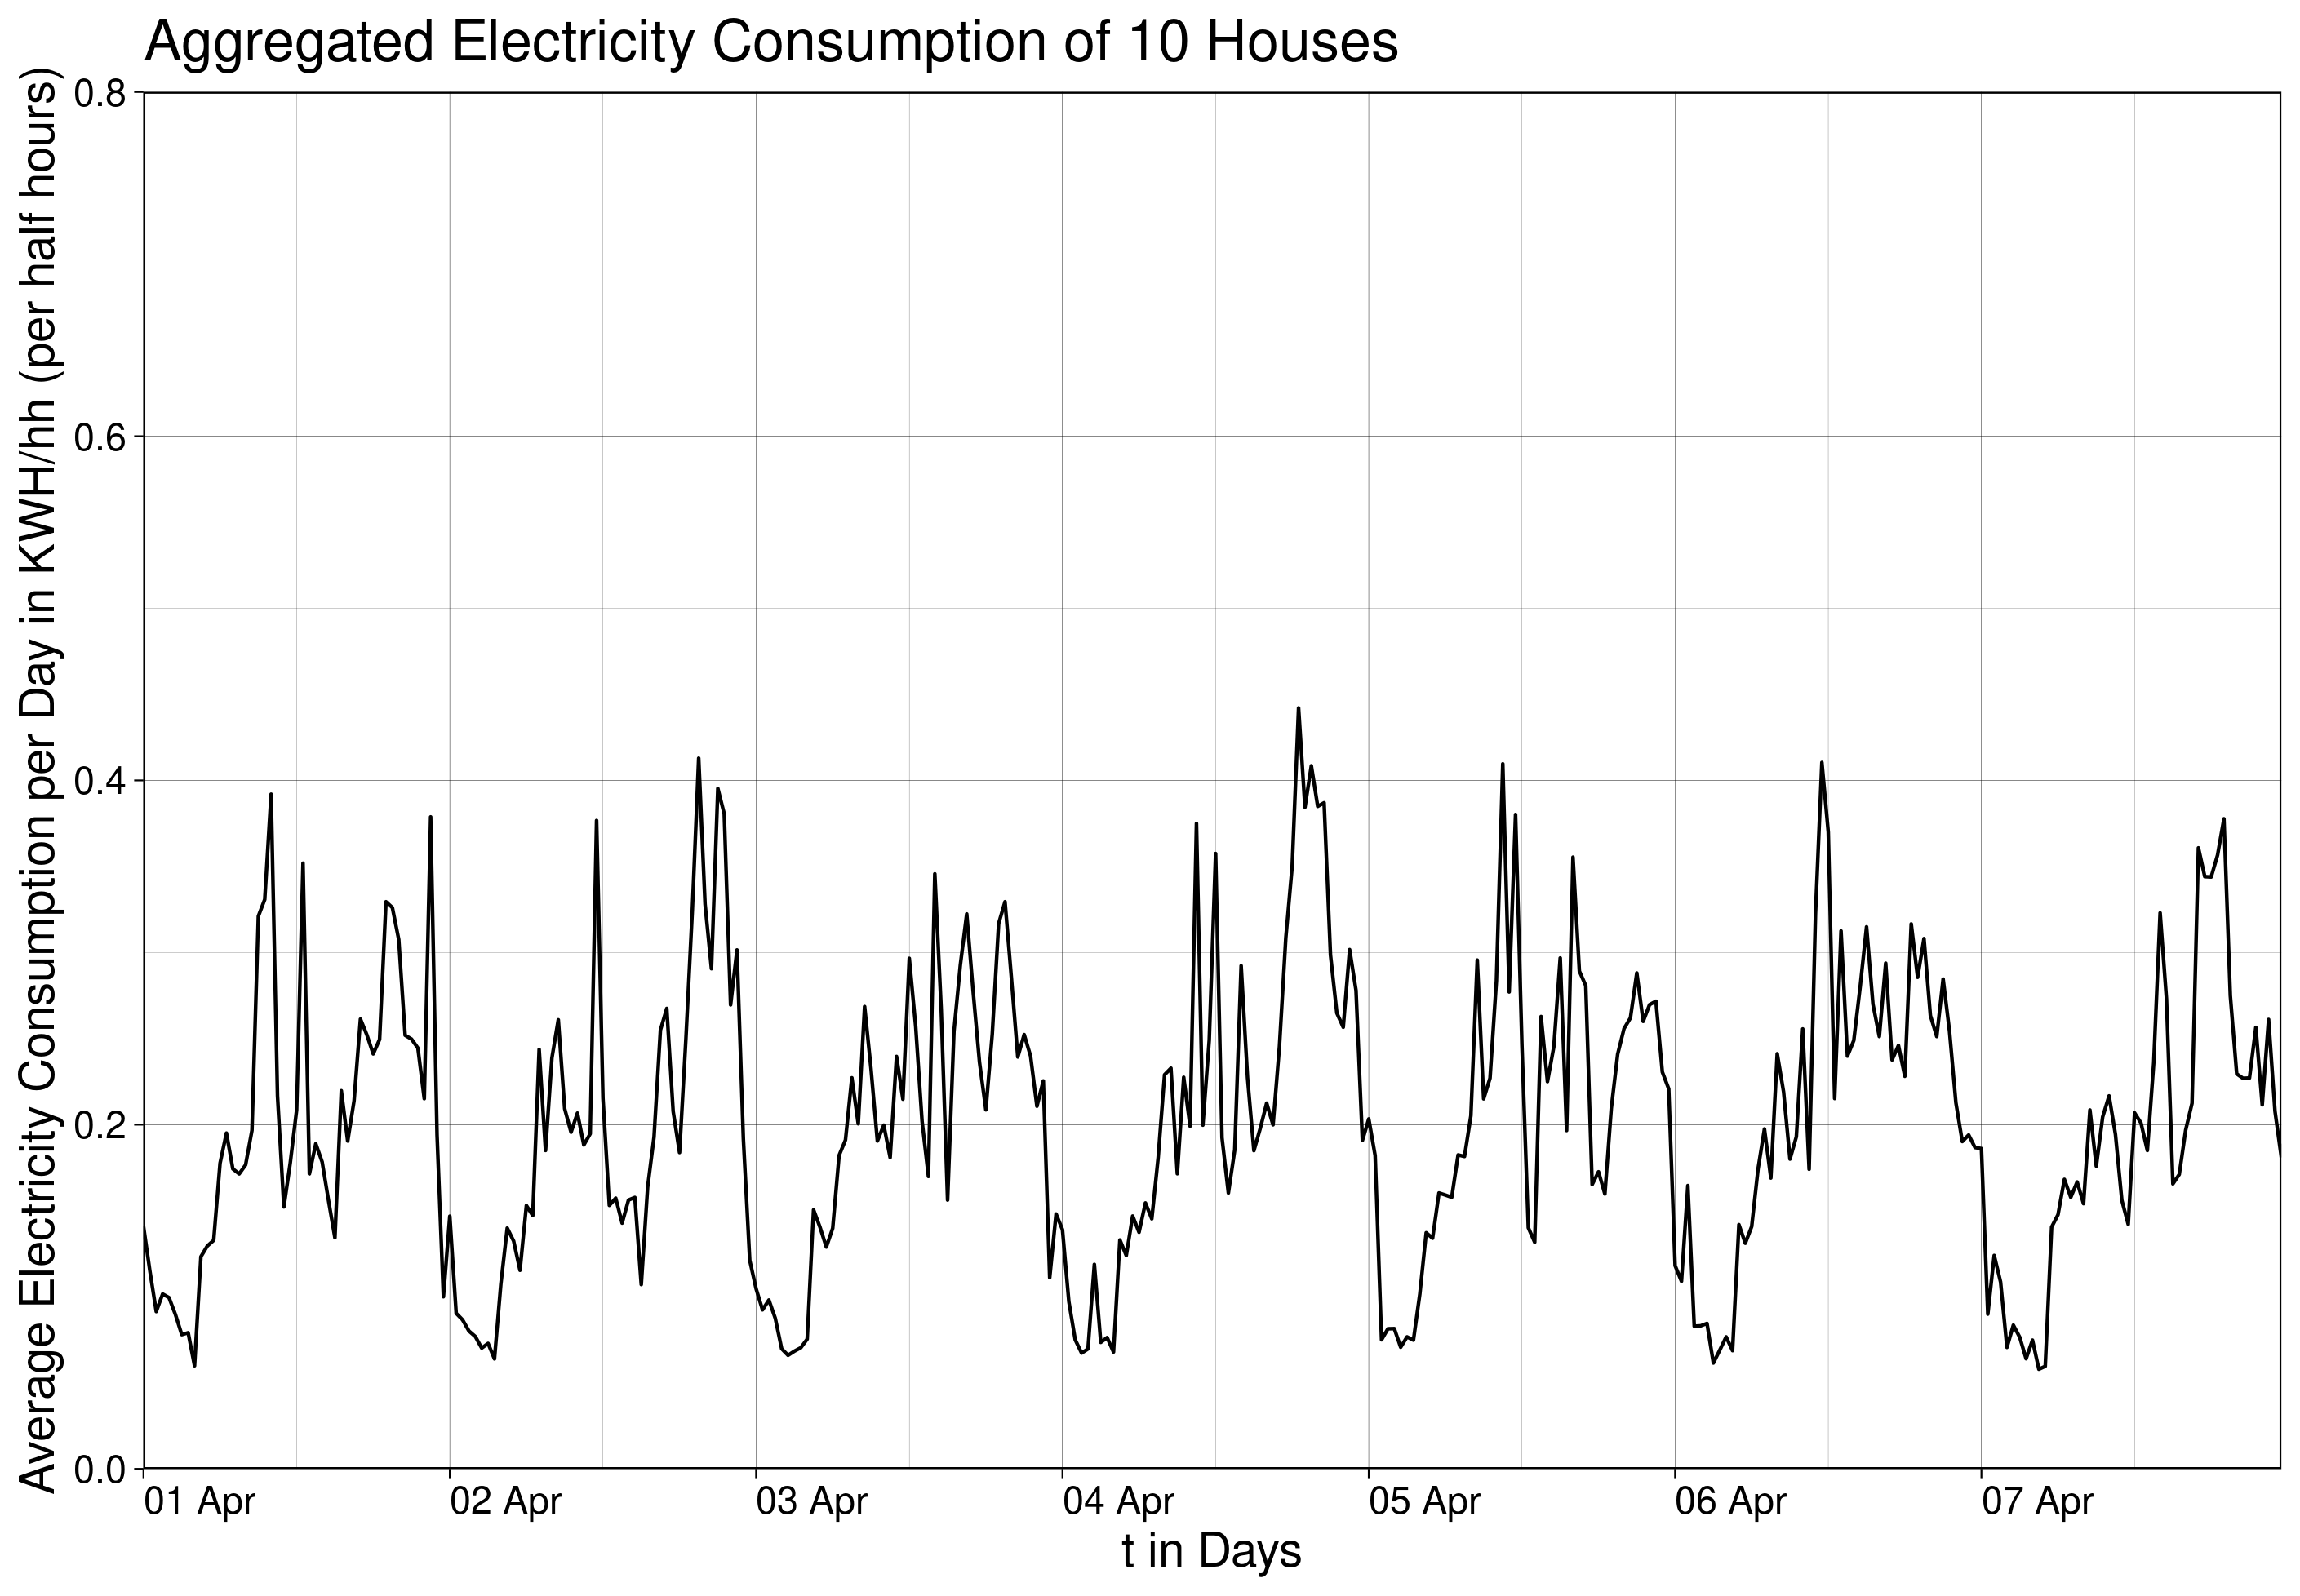
\includegraphics[width=0.85\textwidth]{images/Aggregated Electricity Consumption of 10 Houses5.png}
\caption[Aggregated Electricity Consumption of 10 Houses of the 2nd Experiment]{}
\label{img:10_Houses_weekly}
\end{figure}
\clearpage
}
\afterpage{%
\begin{figure}[!p]
\centering
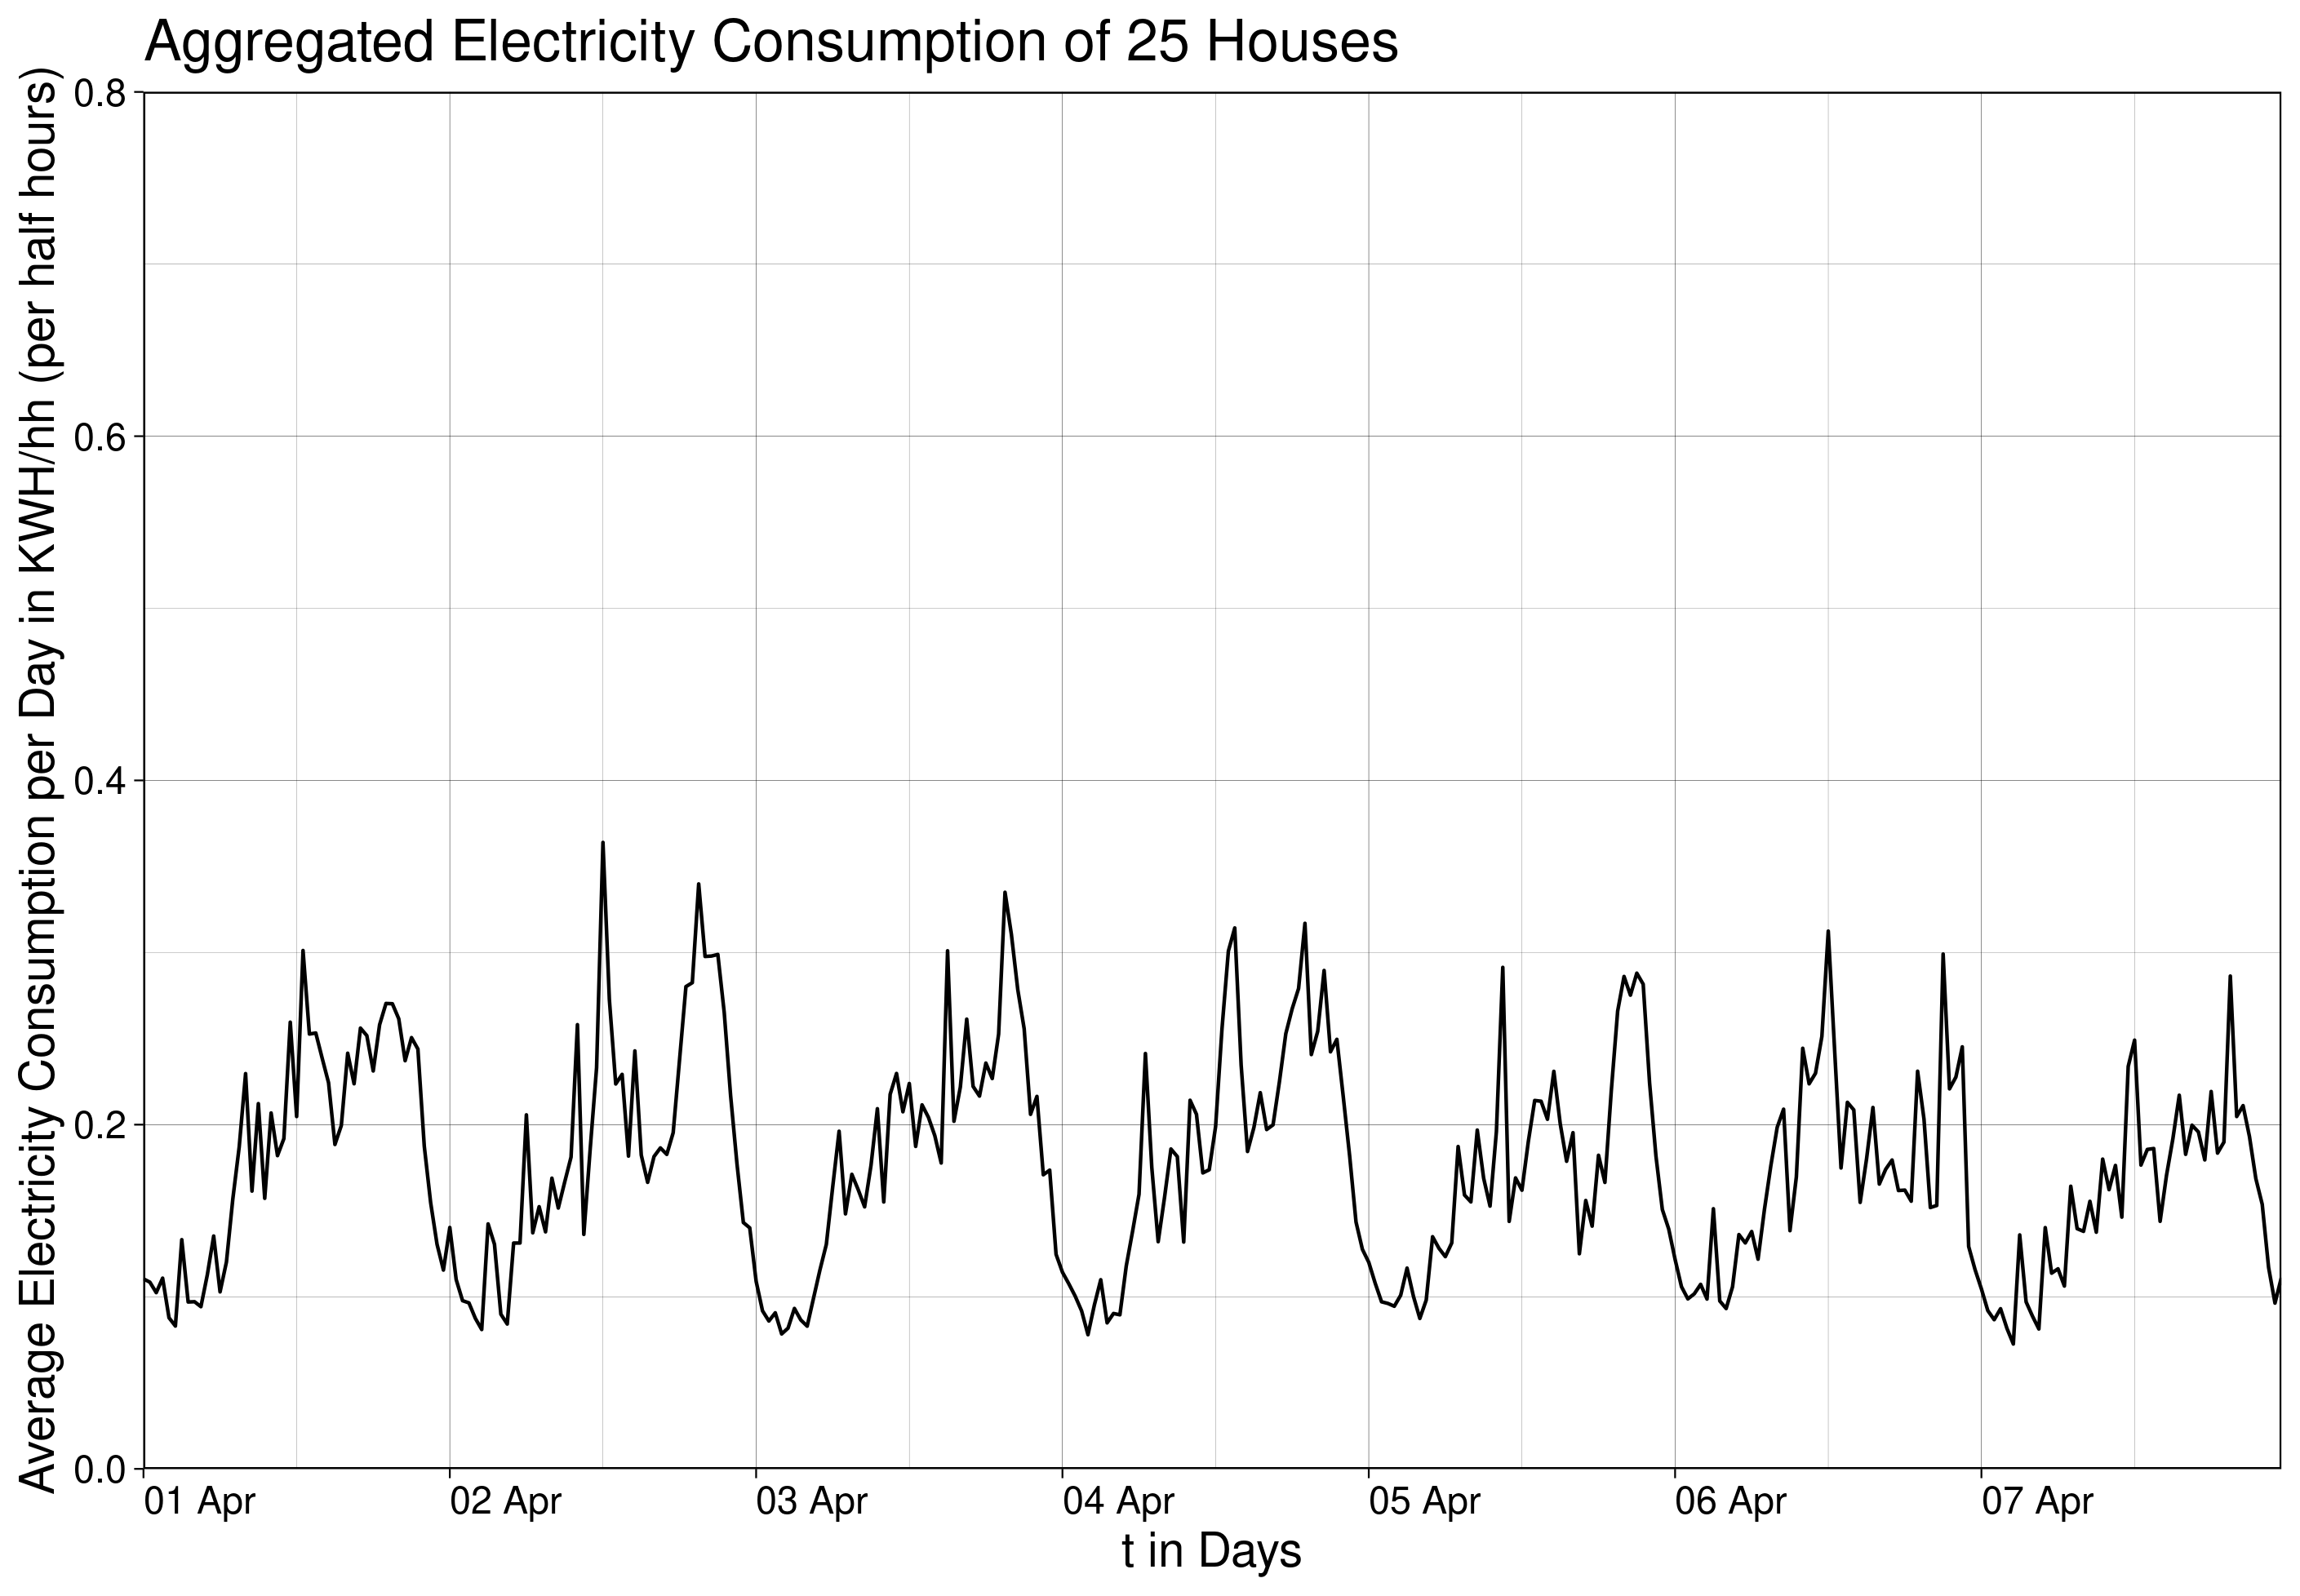
\includegraphics[width=0.85\textwidth]{images/Aggregated Electricity Consumption of 25 Houses5.png}
\caption[Aggregated Electricity Consumption of 25 Houses of the 2nd Experiment]{}
\label{img:25_Houses_weekly}
\end{figure}
\begin{figure}[!p]
\centering
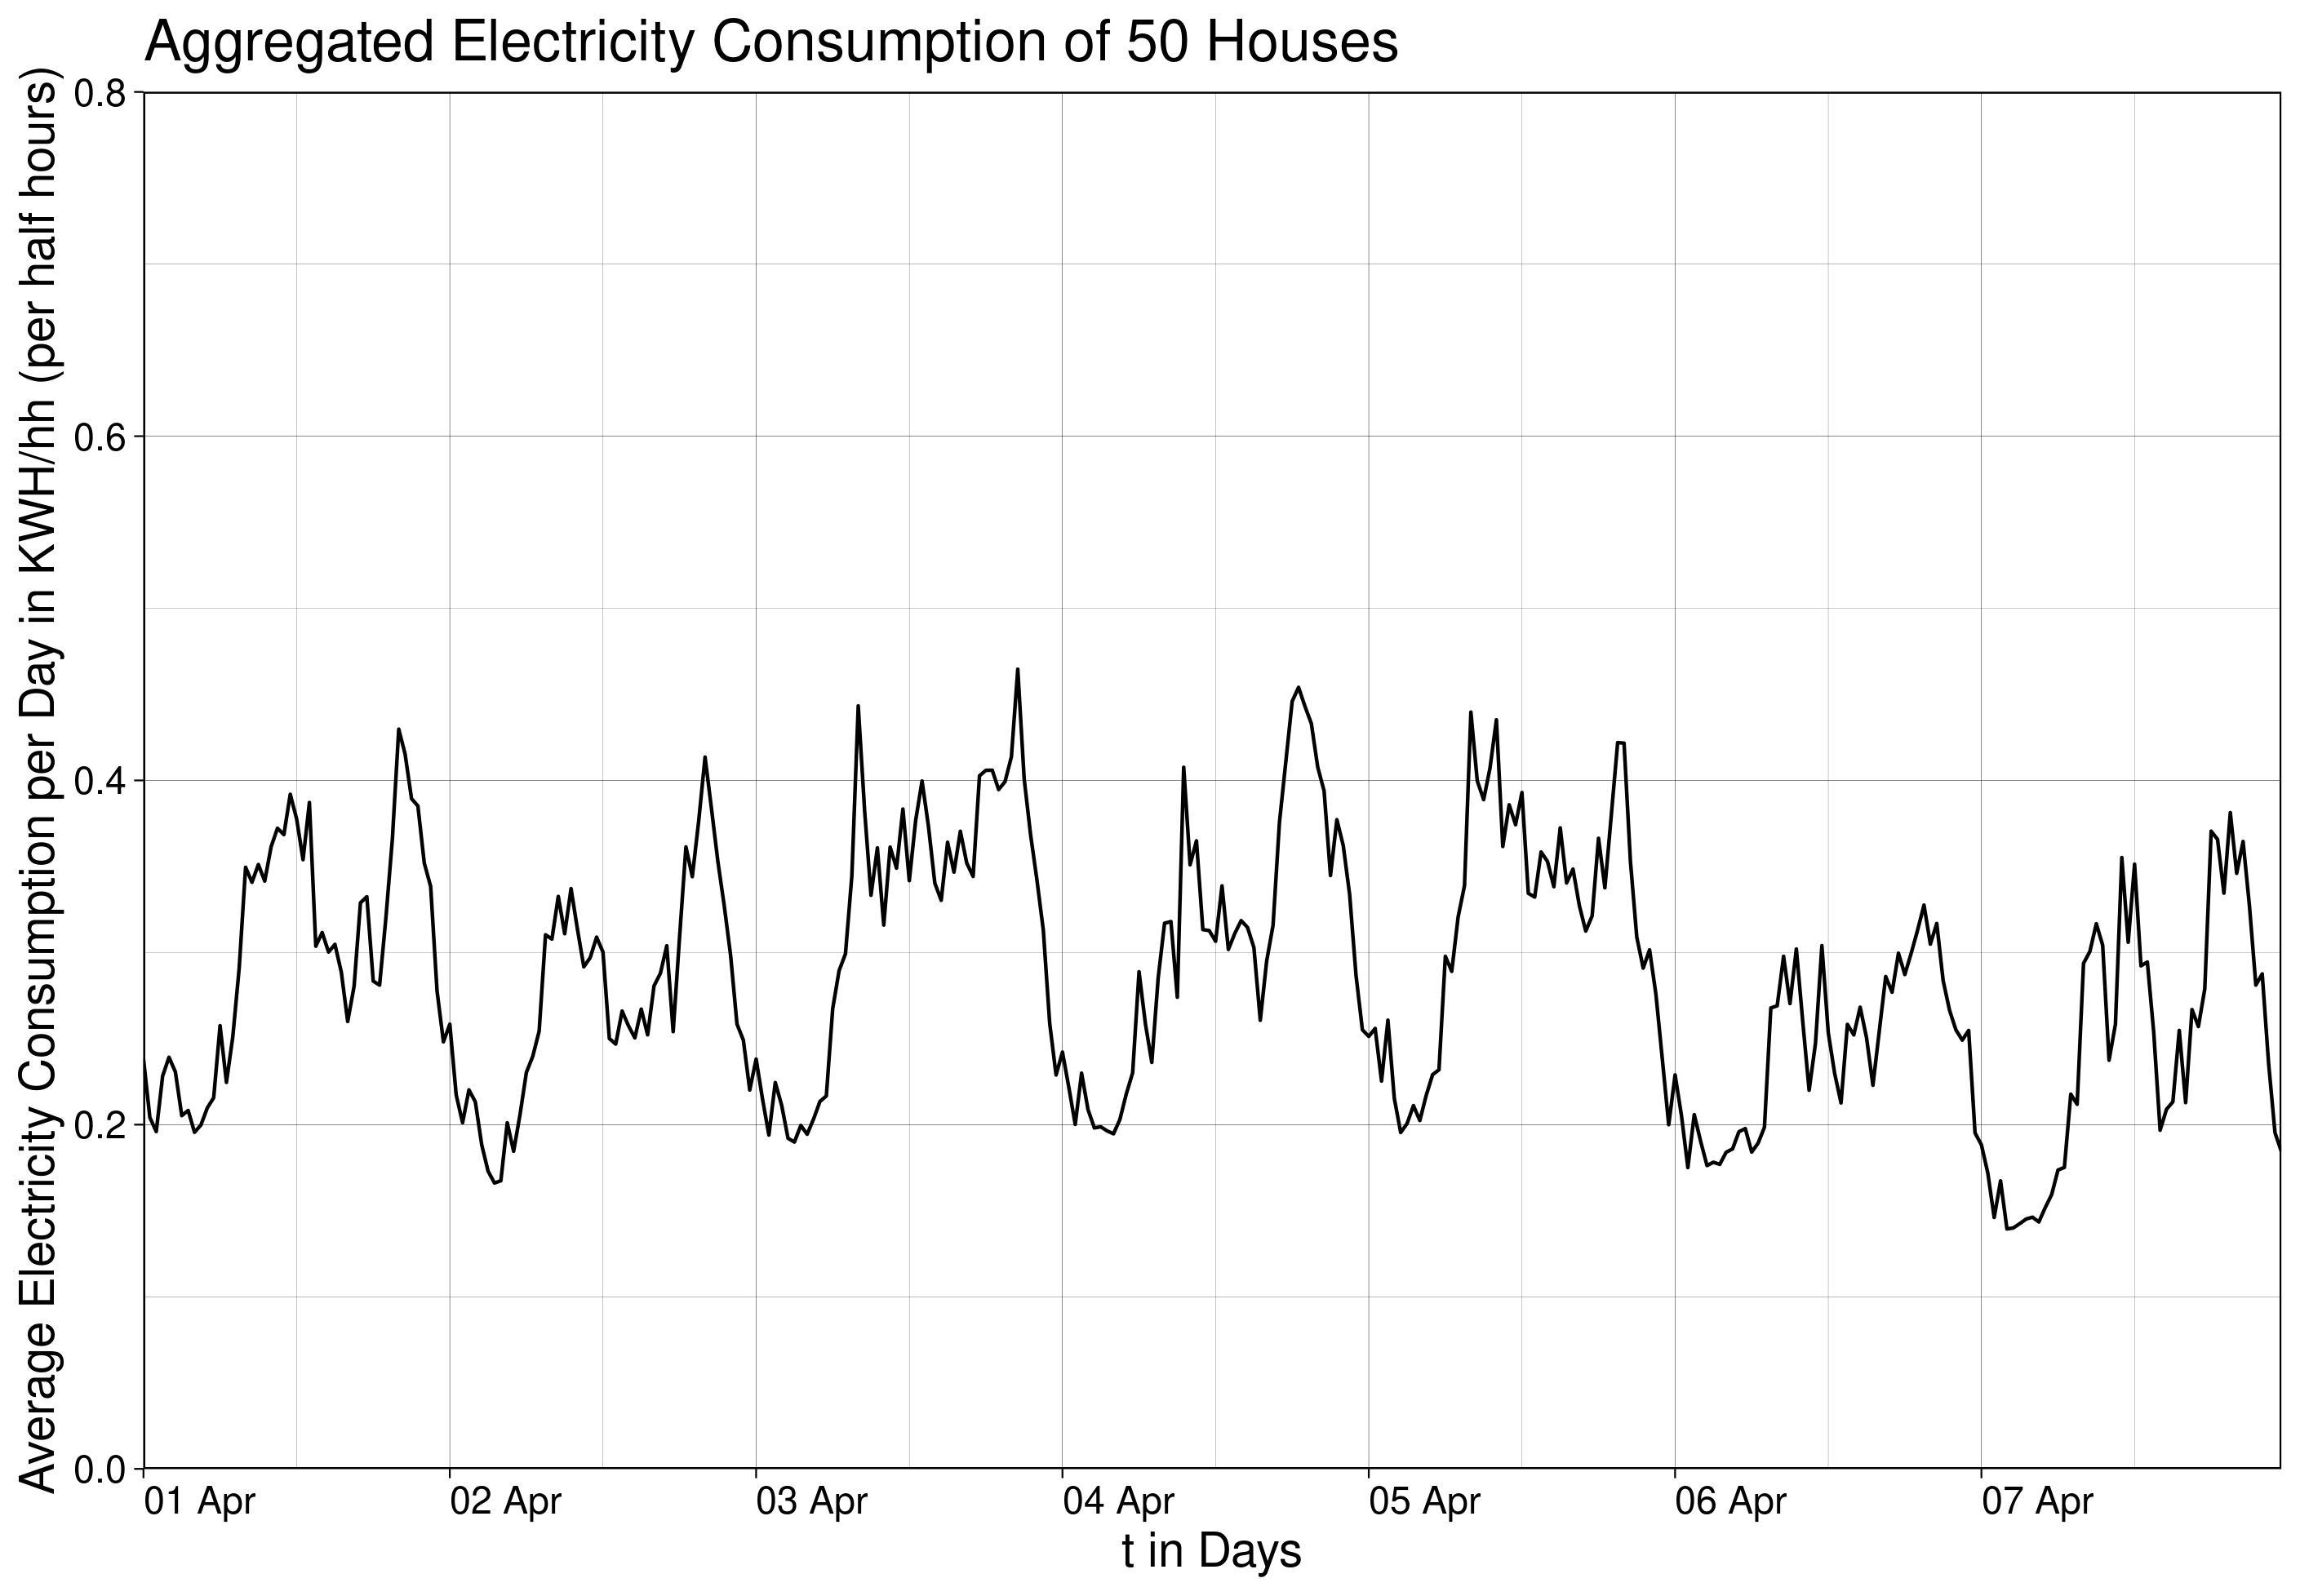
\includegraphics[width=0.85\textwidth]{images/Aggregated Electricity Consumption of 50 Houses5.png}
\caption[Aggregated Electricity Consumption of 50 Houses of the 2nd Experiment]{}
\label{img:50_Houses_weekly}
\end{figure}
\clearpage
}
\afterpage{%
\begin{figure}[!p]
\centering
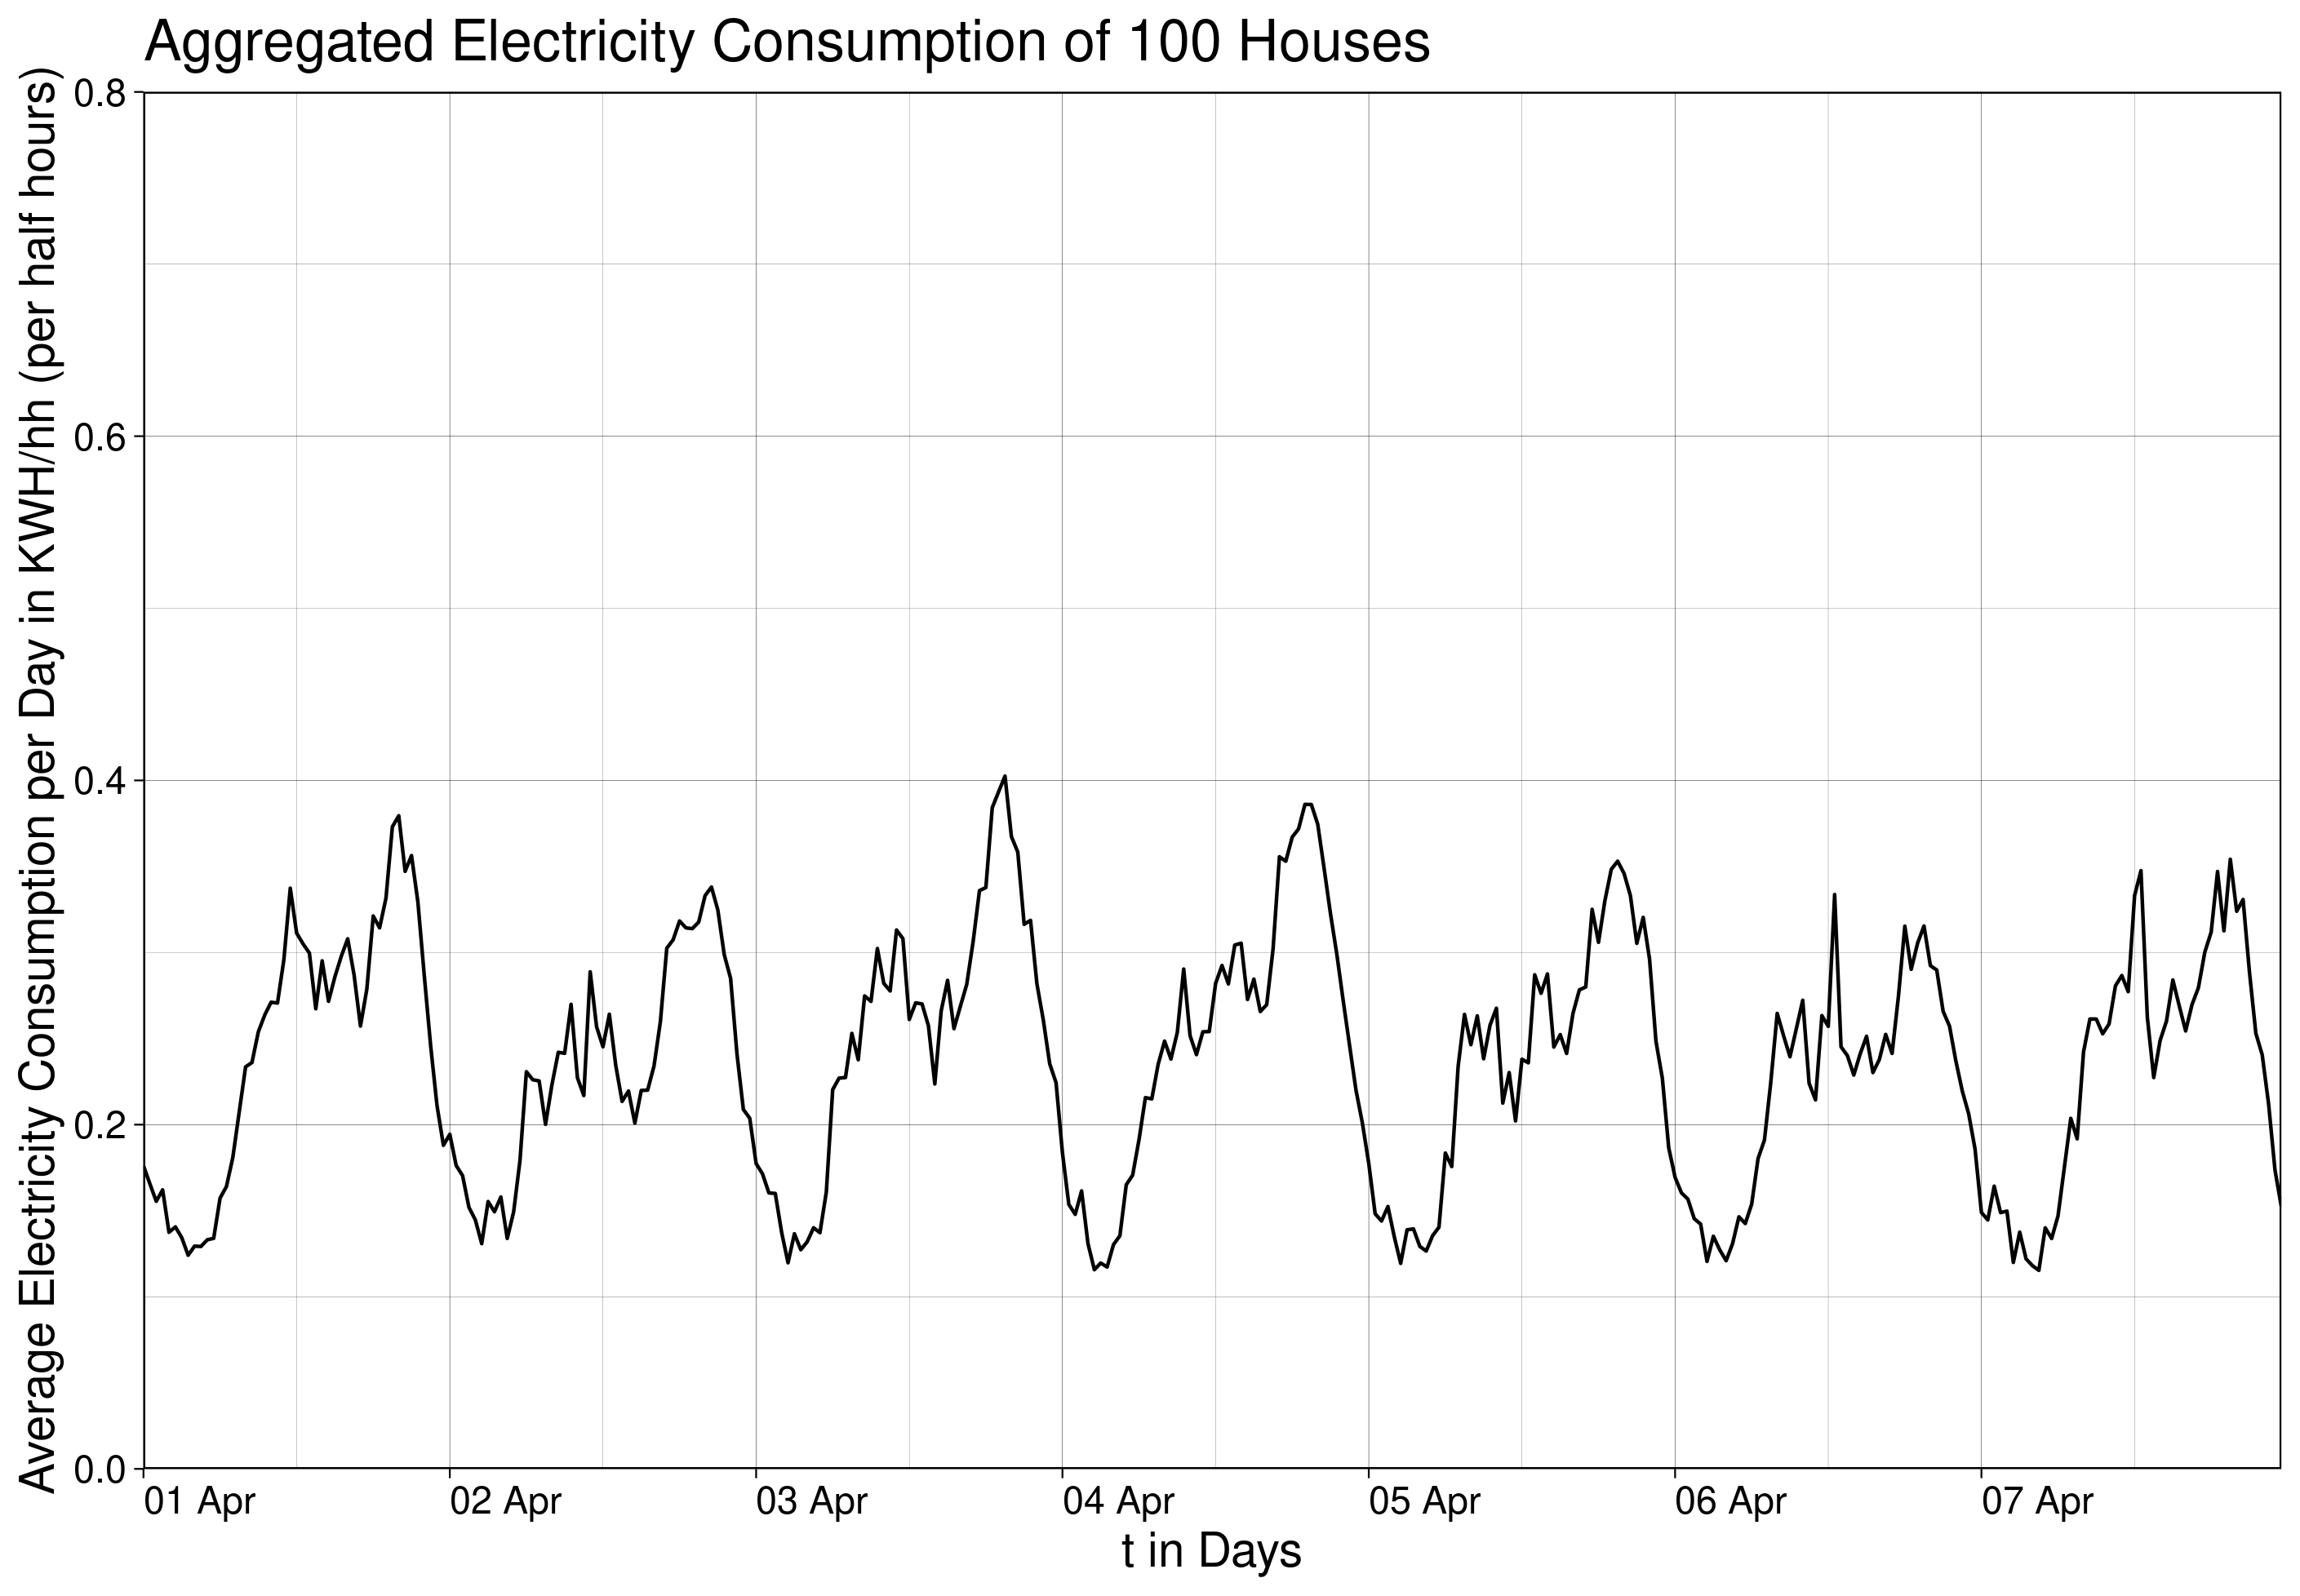
\includegraphics[width=0.85\textwidth]{images/Aggregated Electricity Consumption of 100 Houses5.png}
\caption[Aggregated Electricity Consumption of 100 Houses of the 2nd Experiment]{}
\label{img:100_Houses_weekly}
\end{figure}
\begin{figure}[!p]
\centering
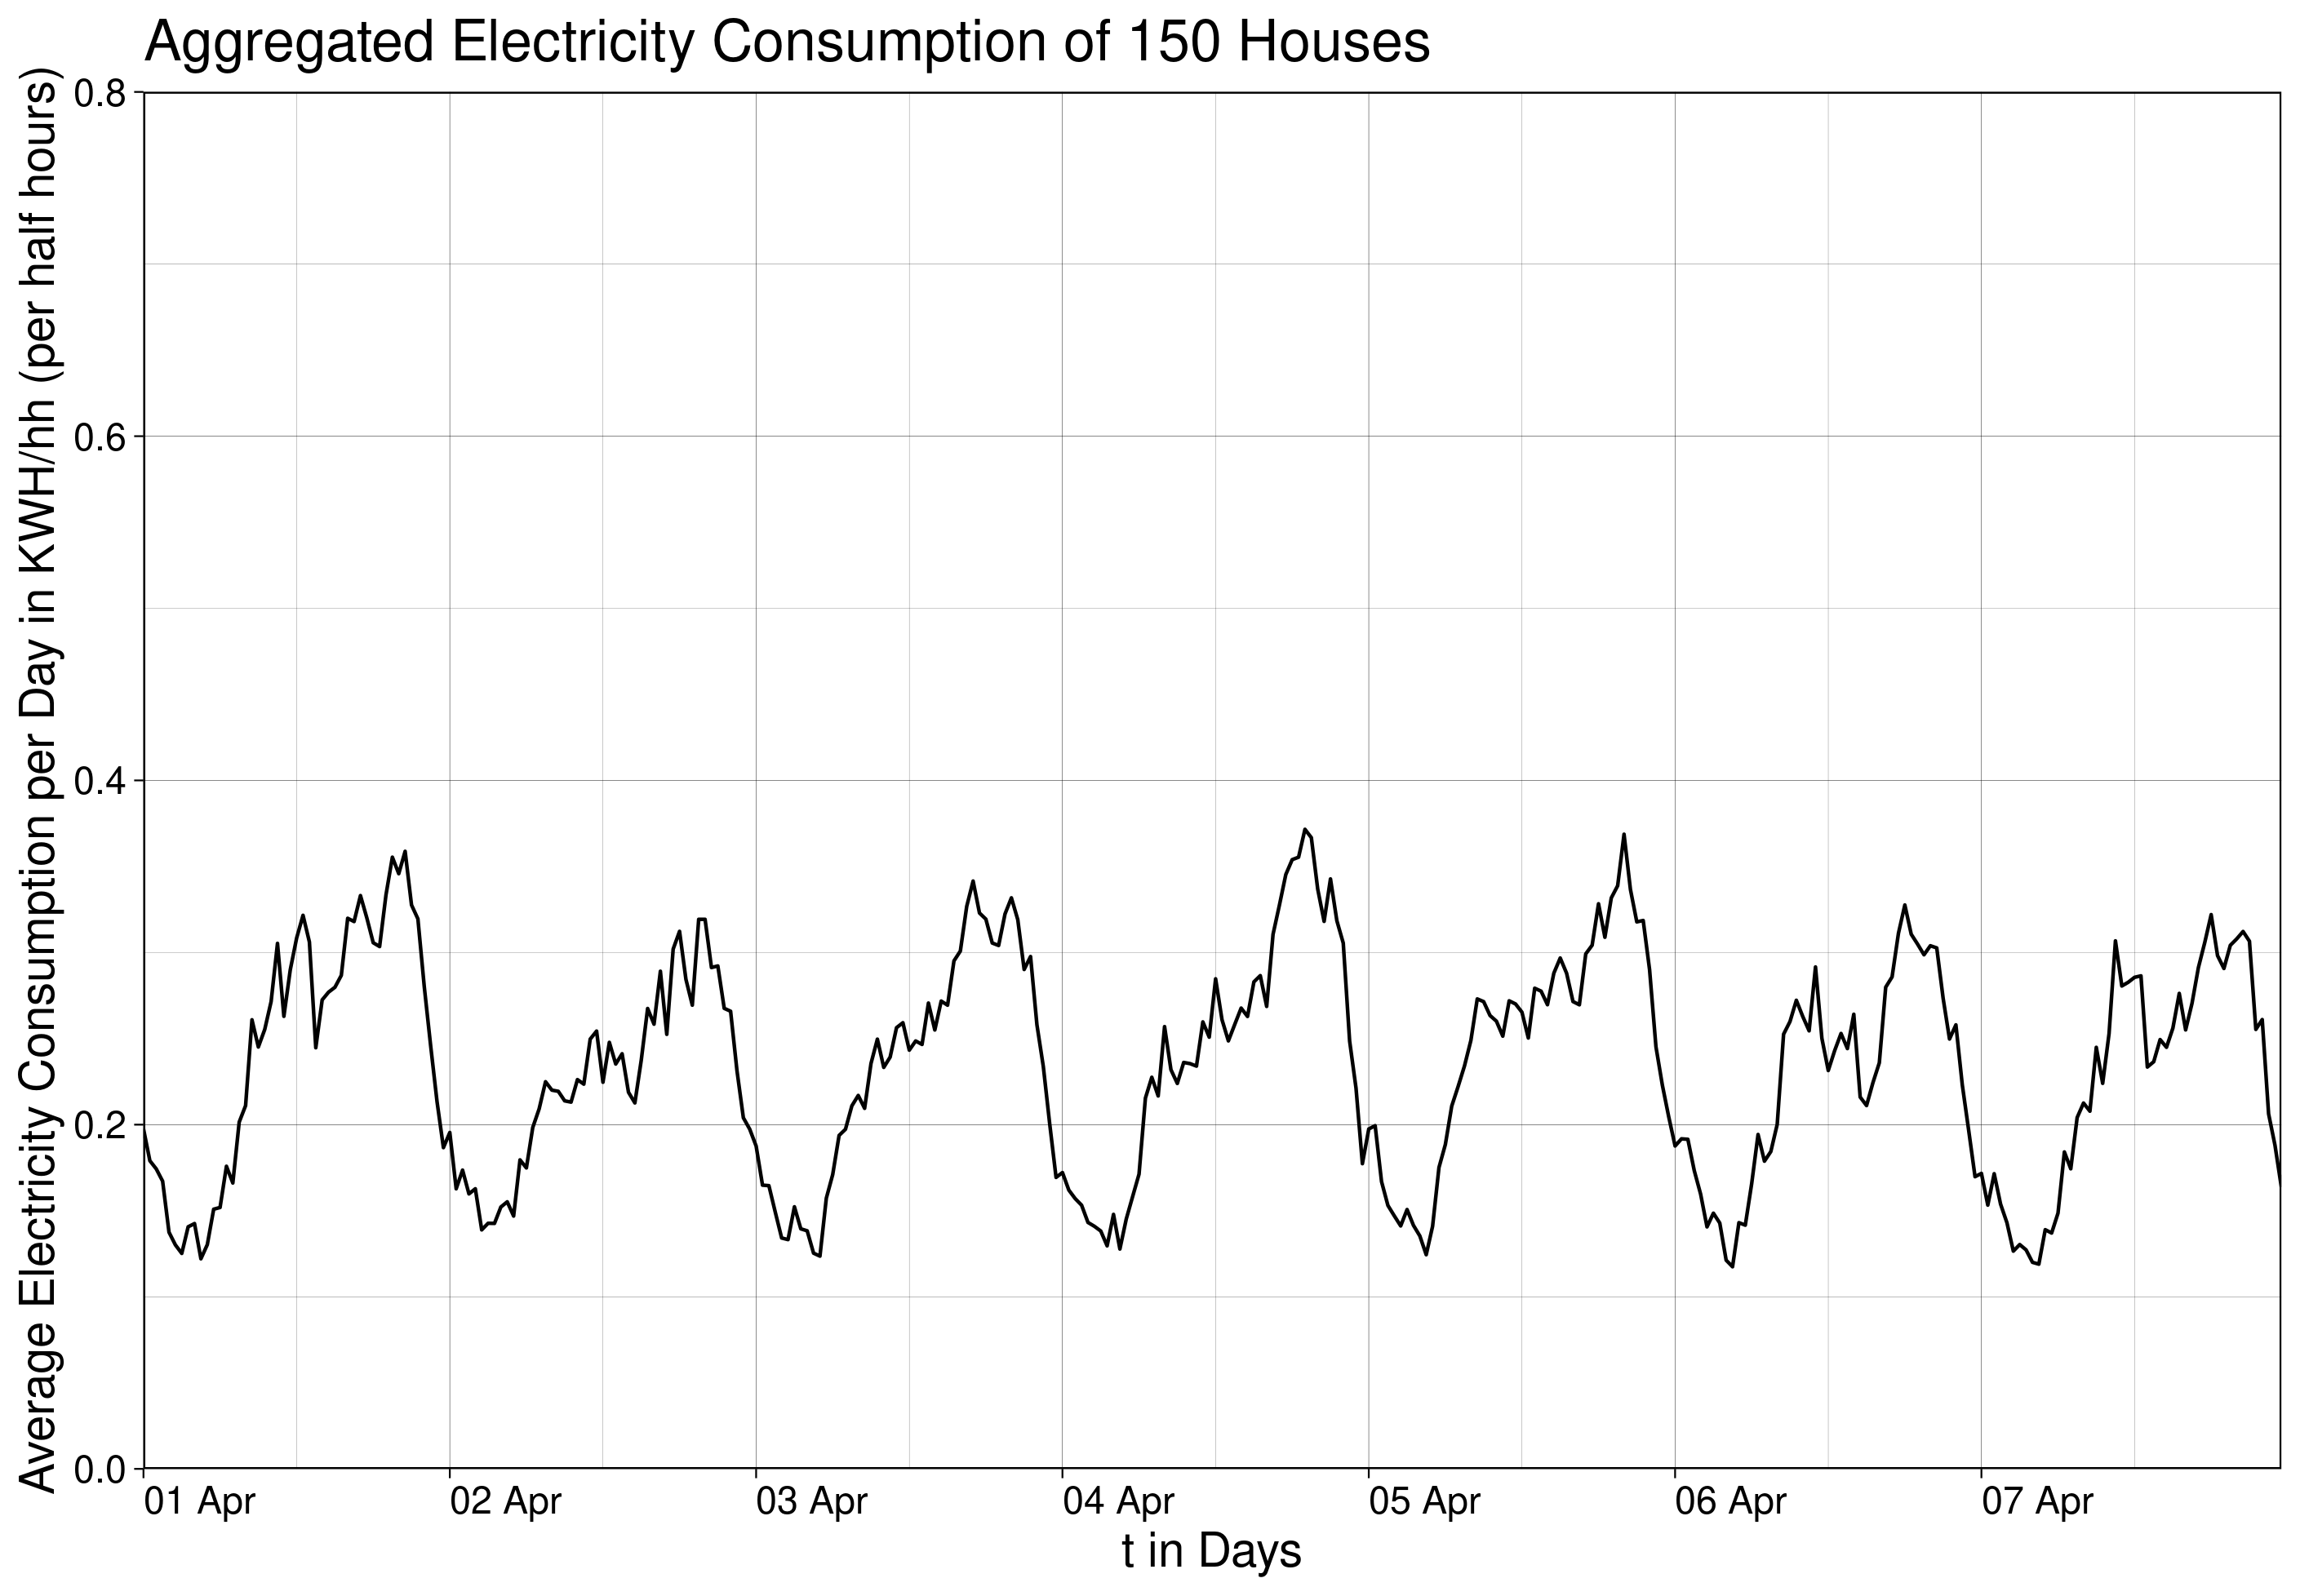
\includegraphics[width=0.85\textwidth]{images/Aggregated Electricity Consumption of 150 Houses5.png}
\caption[Aggregated Electricity Consumption of 150 Houses of the 2nd Experiment]{}
\label{img:150_houses_weekly}
\end{figure}
\clearpage
}
\afterpage{%
\begin{figure}[!p]
\centering
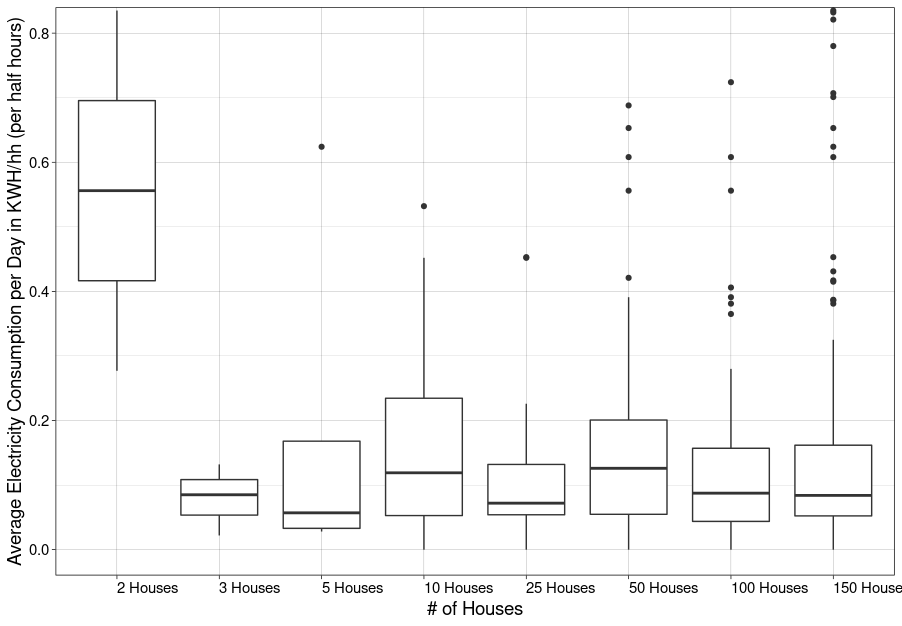
\includegraphics[width=0.85\textwidth]{images/Boxplot_test4.png}
\caption[Boxplot of the first Week]{}
\label{img:boxplot_first}
\end{figure}
\begin{figure}[!p]
\centering
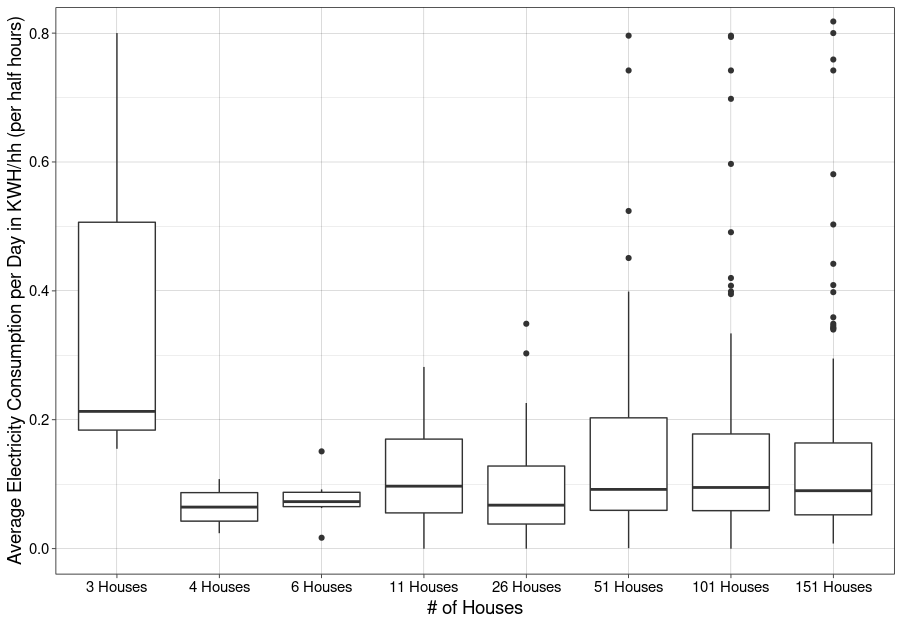
\includegraphics[width=0.85\textwidth]{images/boxplot_2nd_week.png}
\caption[Boxplot of the second Week]{}
\label{img:boxplot_second}
\end{figure}
\clearpage
}

\afterpage{%
\begin{figure}[!p]
\centering
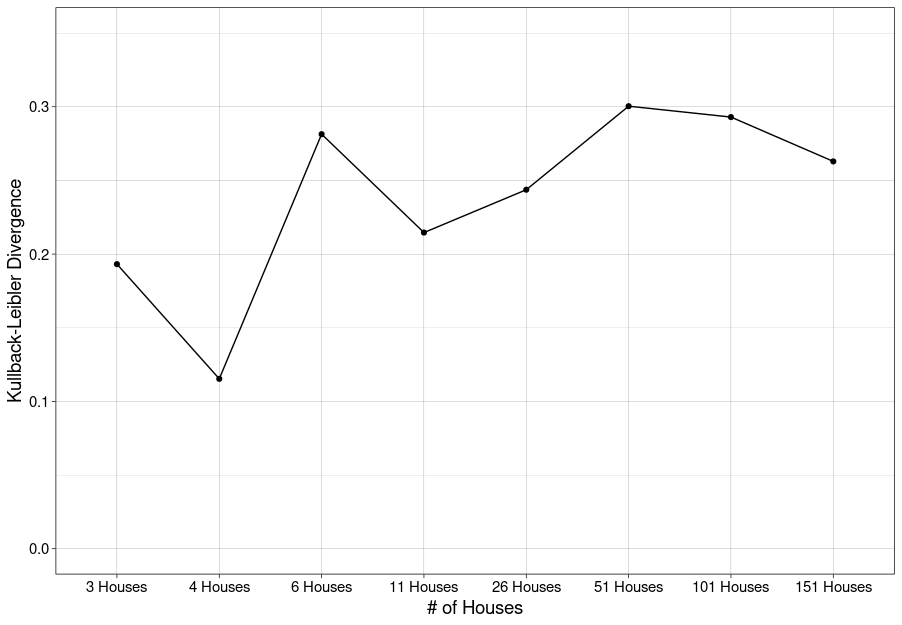
\includegraphics[width=0.85\textwidth]{images/KLD_Test2.png}
\caption[Kullback Leibler Divergence]{Kullback Leibler Divergence}
\label{img:KLD}
\end{figure}
\begin{figure}[!p]
\centering
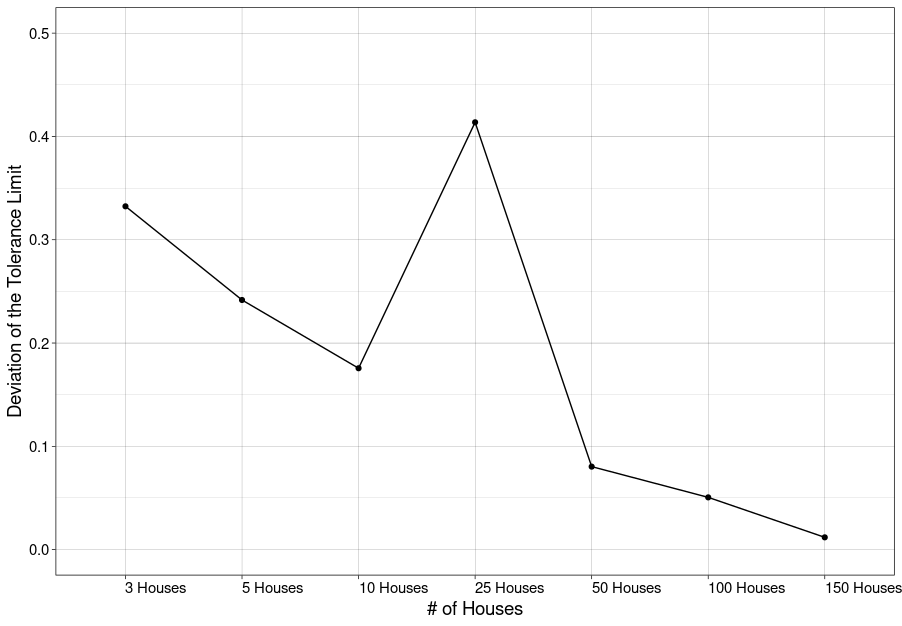
\includegraphics[width=0.85\textwidth]{images/Deviation1.png}
\caption[Deviation of the 2nd Experiment]{Deviation}
\label{img:Dev_2nd}
\end{figure}
\clearpage
}
\afterpage{%
\begin{figure}[!p]
\centering
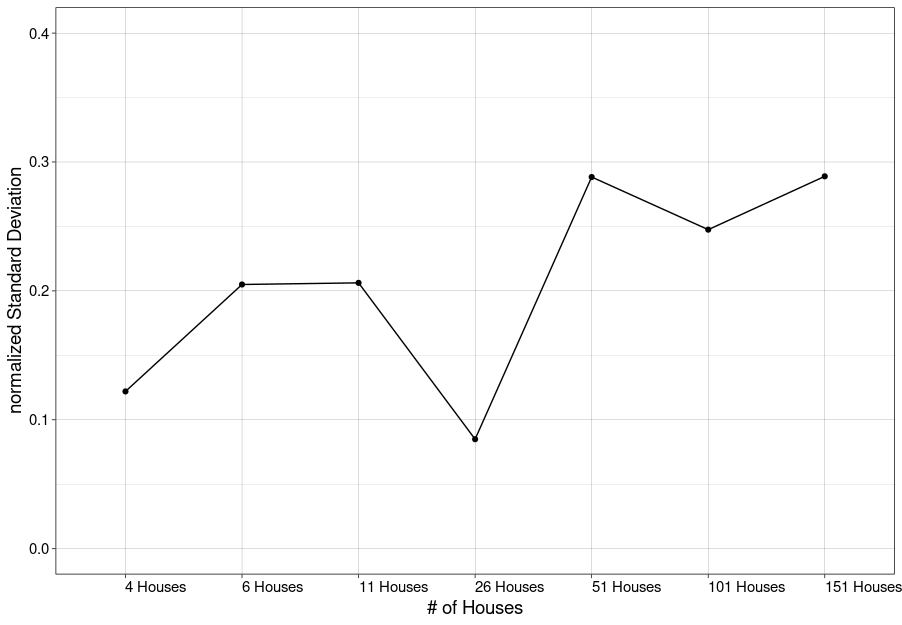
\includegraphics[width=0.85\textwidth]{images/standard_deviation2_test4.png}
\caption[normalized Standard Deviation]{normalized Standard Deviation}
\label{img:SD}
\end{figure}
\clearpage
}

\chapter{Yearlong Experiments}
\enlargethispage{10}
\vspace*{-10\baseline}
\begin{figure}[H]
\centering
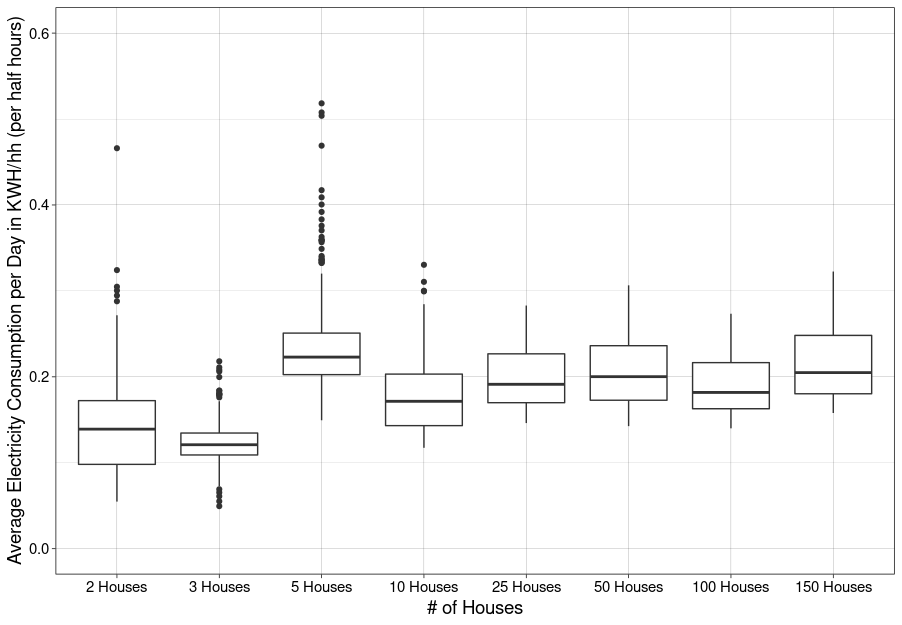
\includegraphics[width=0.8\columnwidth]{images/boxplot_neu_neu.png}
\caption[Boxplots of the Average Base Load]{Boxplots of the Average Base Load}
\label{img:Box}
\centering
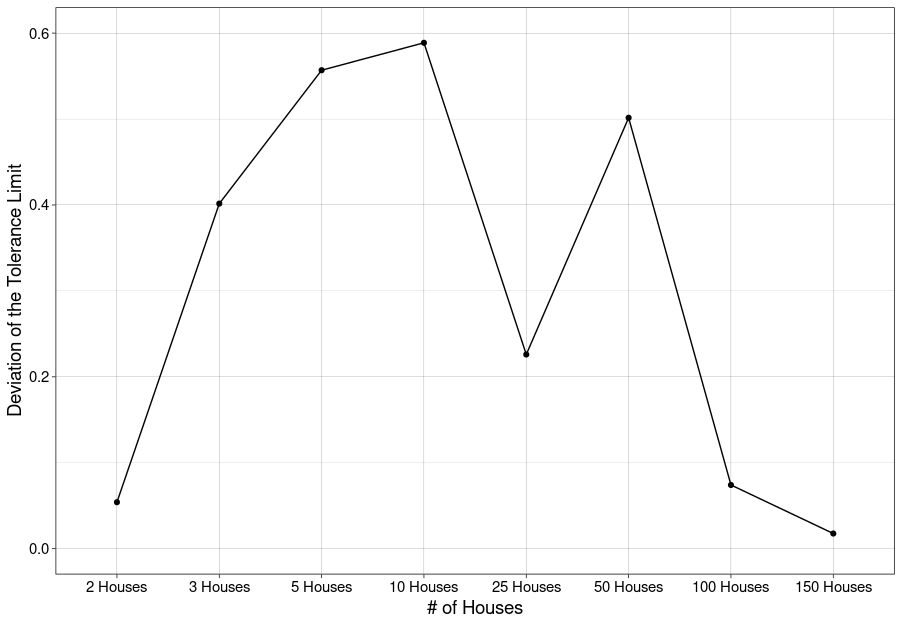
\includegraphics[width=0.8\columnwidth]{images/Deviation_Houses.png}
\caption[Deviation of the Standard Variance]{Deviation of the Standard Variance}
\label{img:Deviation}
\end{figure}
\nopagebreak
%Nachschauen mit den ferien im april bei 2 häusern
%durchschnittliche Mittelwert(von boxplots)
%ergebnisse der abweichung
%versuche wurden 2 mal wiederholt.
\afterpage{%
\begin{figure}[!p]
\centering
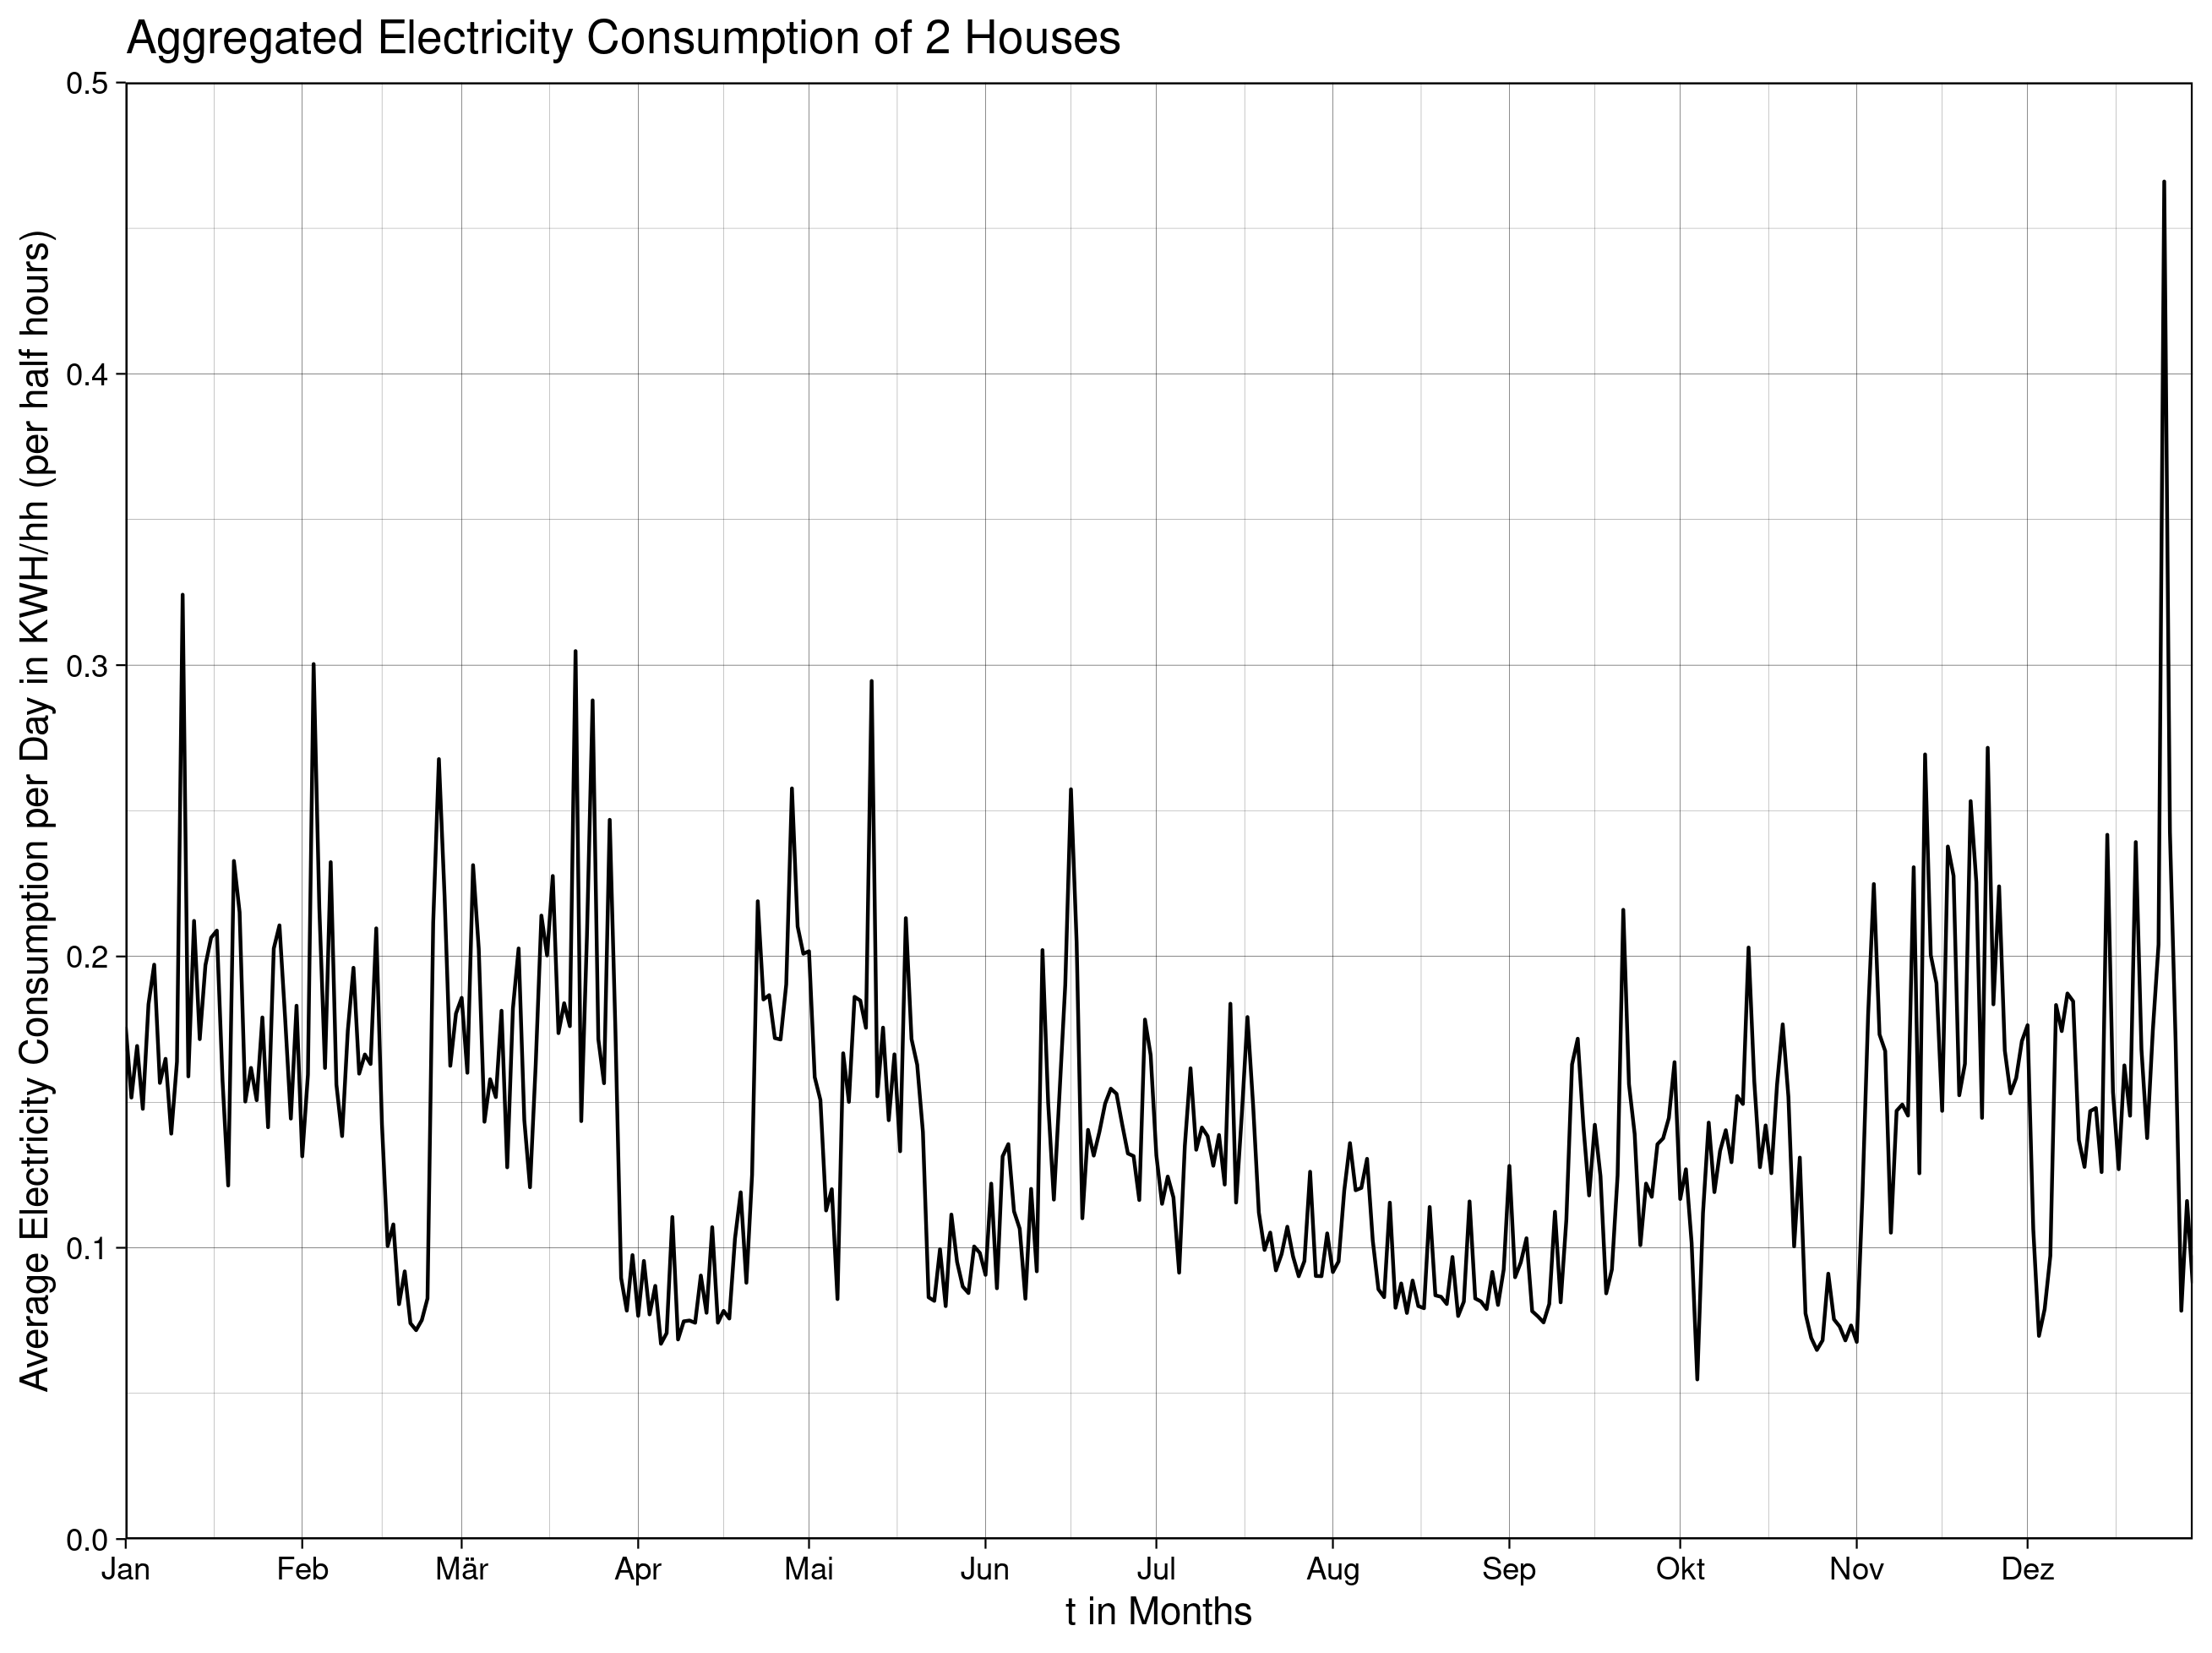
\includegraphics[width=0.85\textwidth]{images/Aggregated Electricity Consumption of 2 Houses.png}
\caption[Aggregated Electricity Consumption of 2 Houses]{}
\label{img:2_Houses}
\end{figure}
\begin{figure}[!p]
\centering
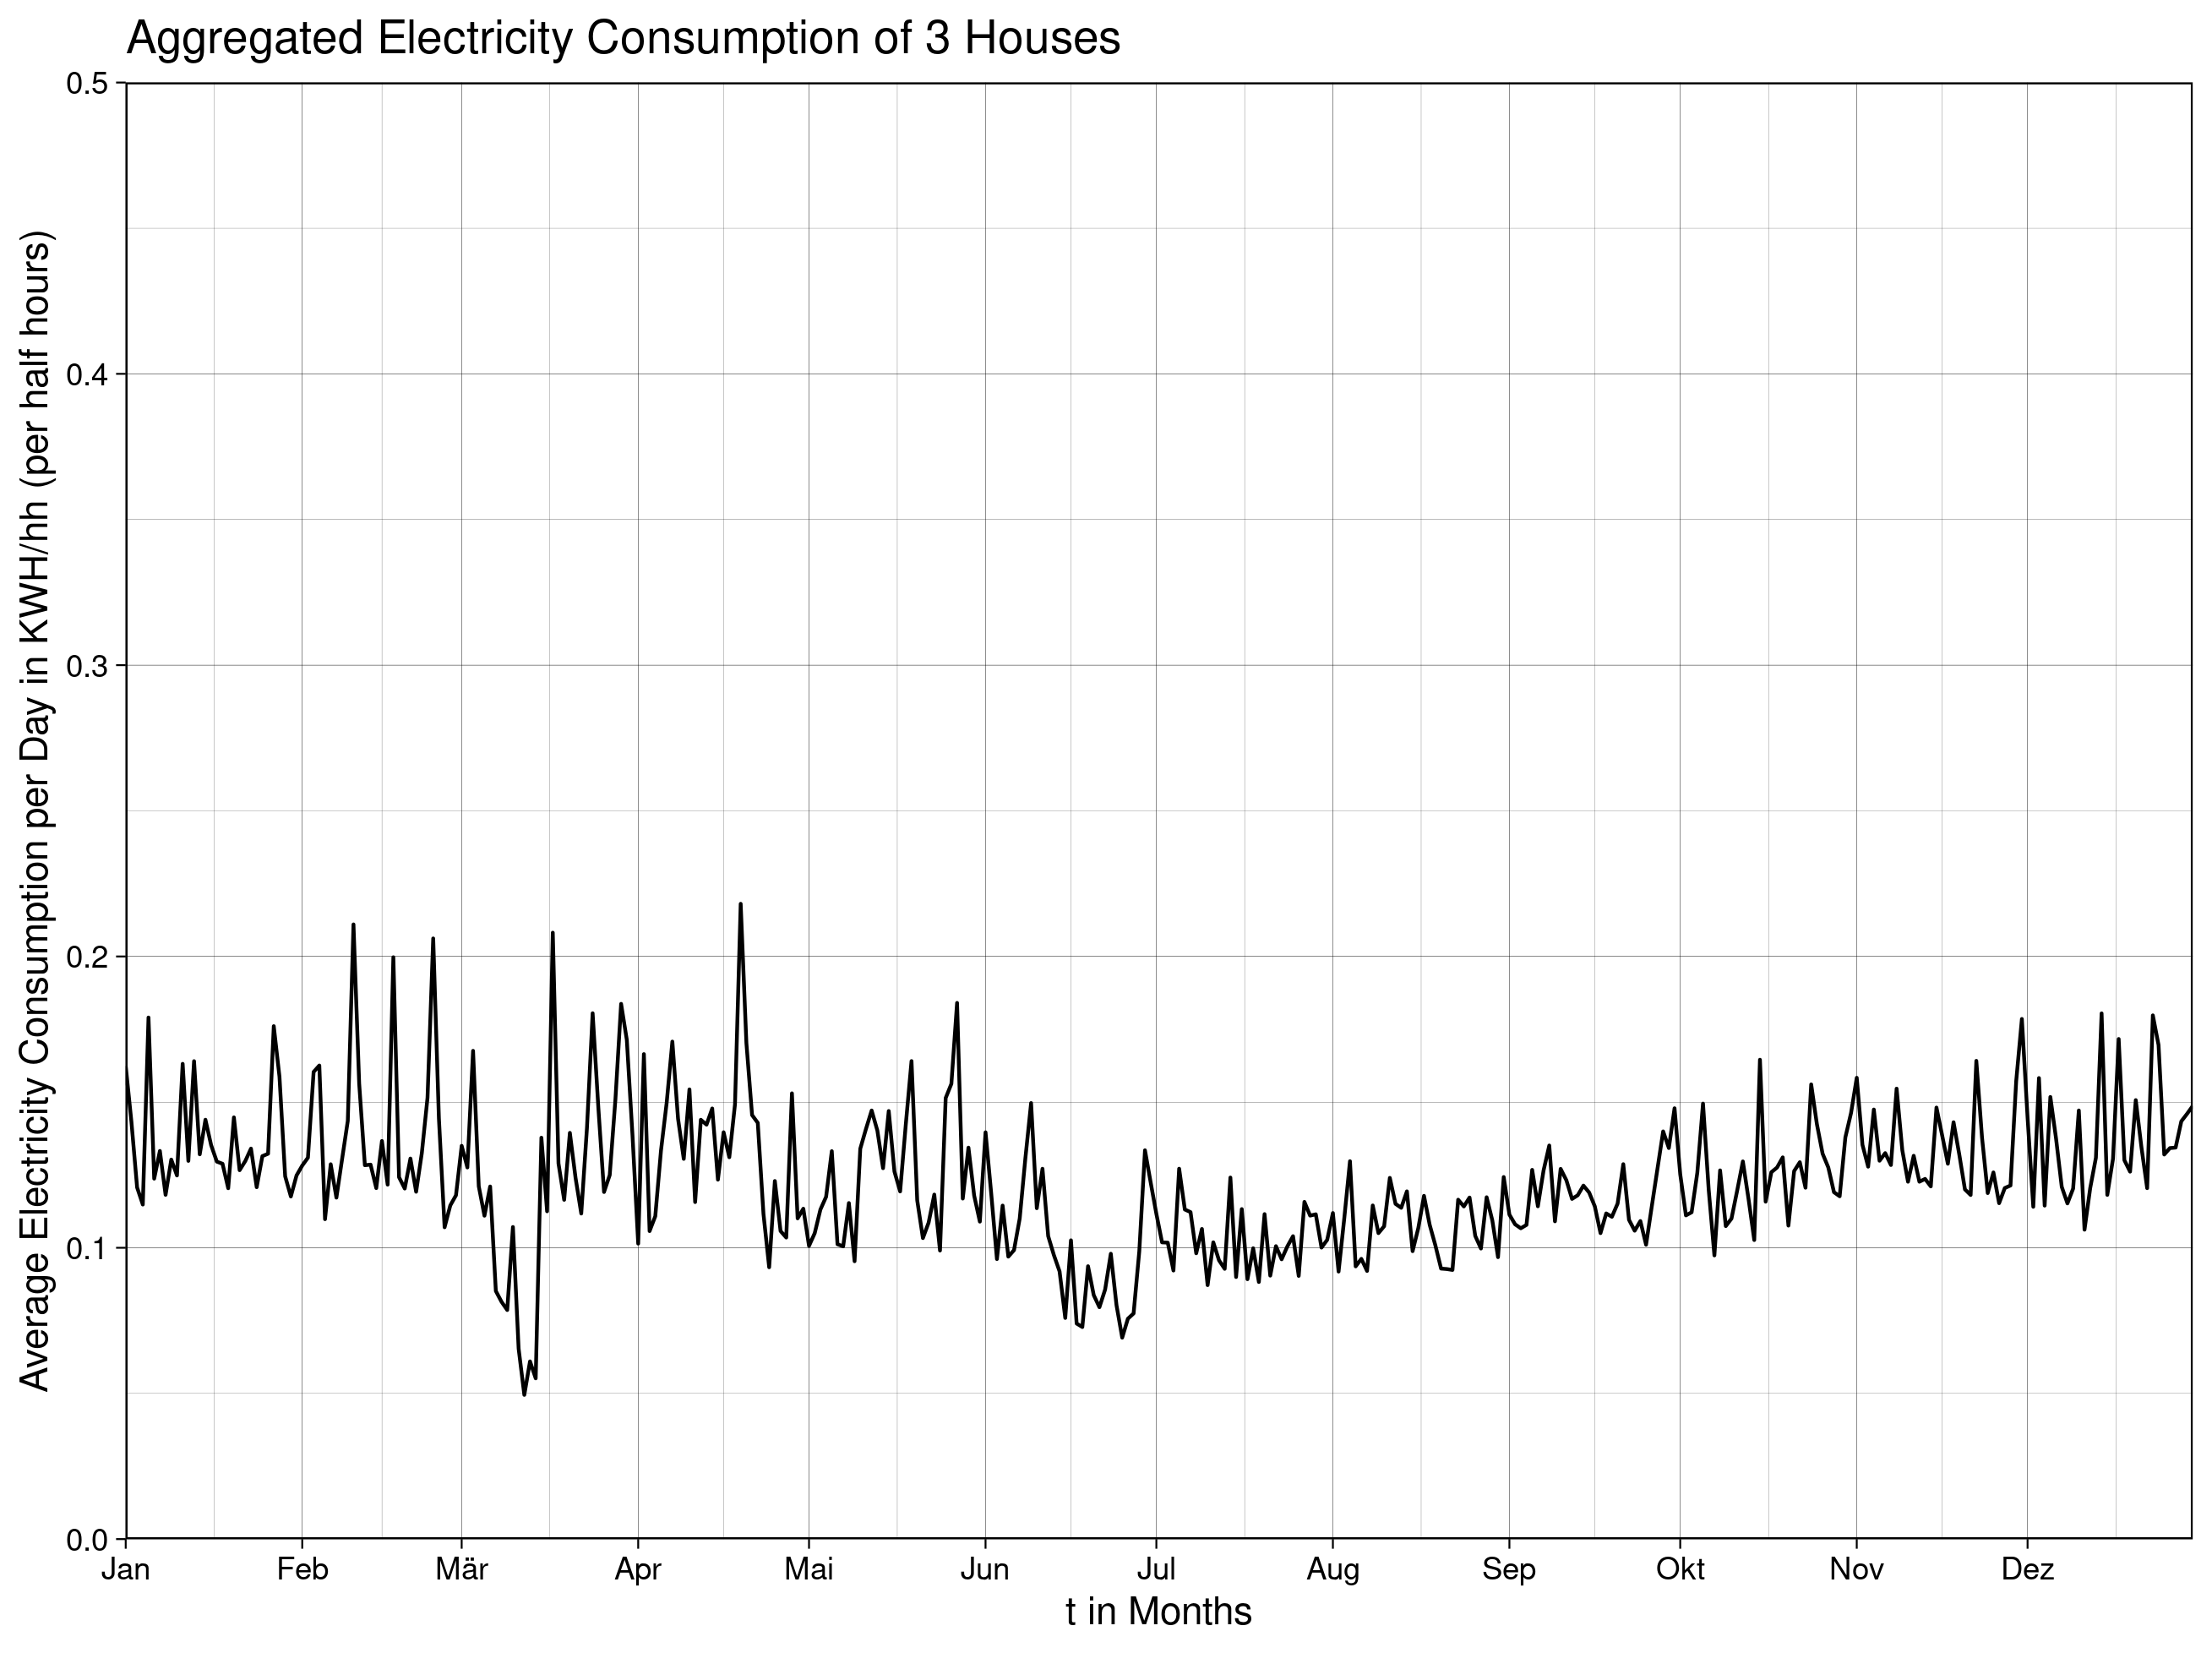
\includegraphics[width=0.85\textwidth]{images/Aggregated Electricity Consumption of 3 Houses.png}
\caption[Aggregated Electricity Consumption of 3 Houses]{}
\label{img:3_Houses}
\end{figure}
\clearpage
}
\afterpage{%
\begin{figure}[!p]
\centering
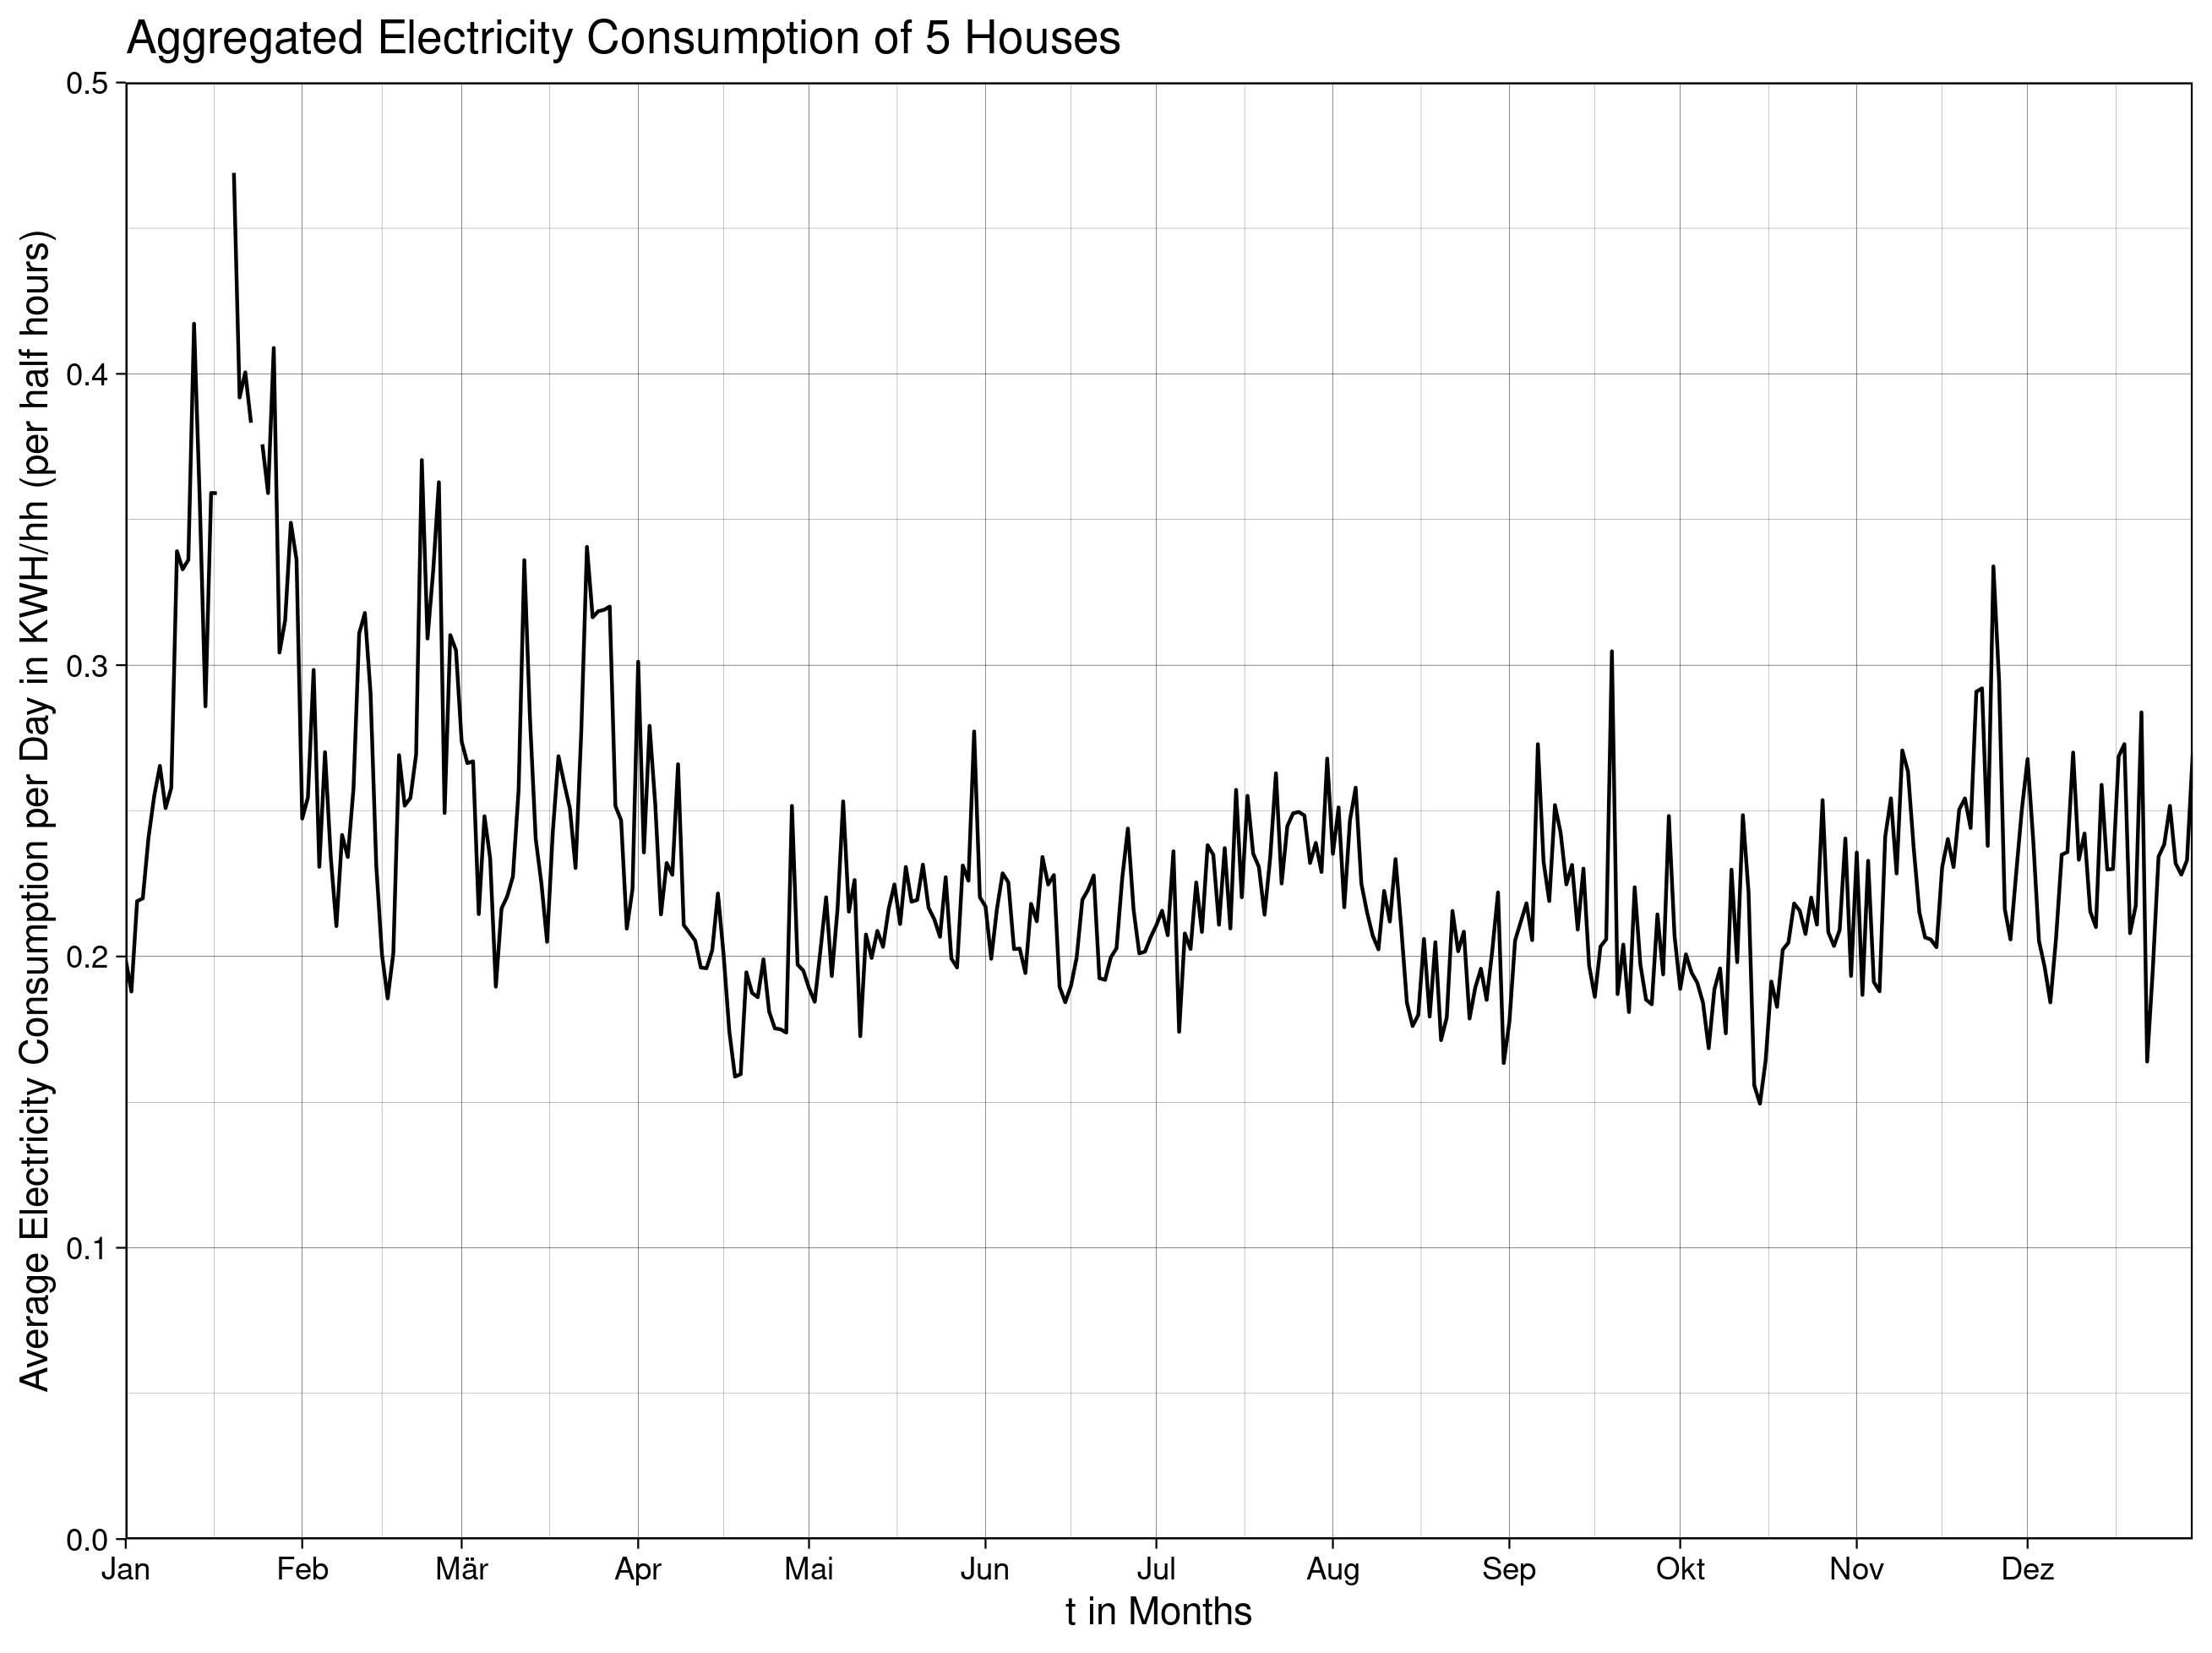
\includegraphics[width=0.85\textwidth]{images/Aggregated Electricity Consumption of 5 Houses.png}
\caption[Aggregated Electricity Consumption of 5 Houses]{}
\label{img:5_Houses}
\end{figure}
\begin{figure}[!p]
\centering
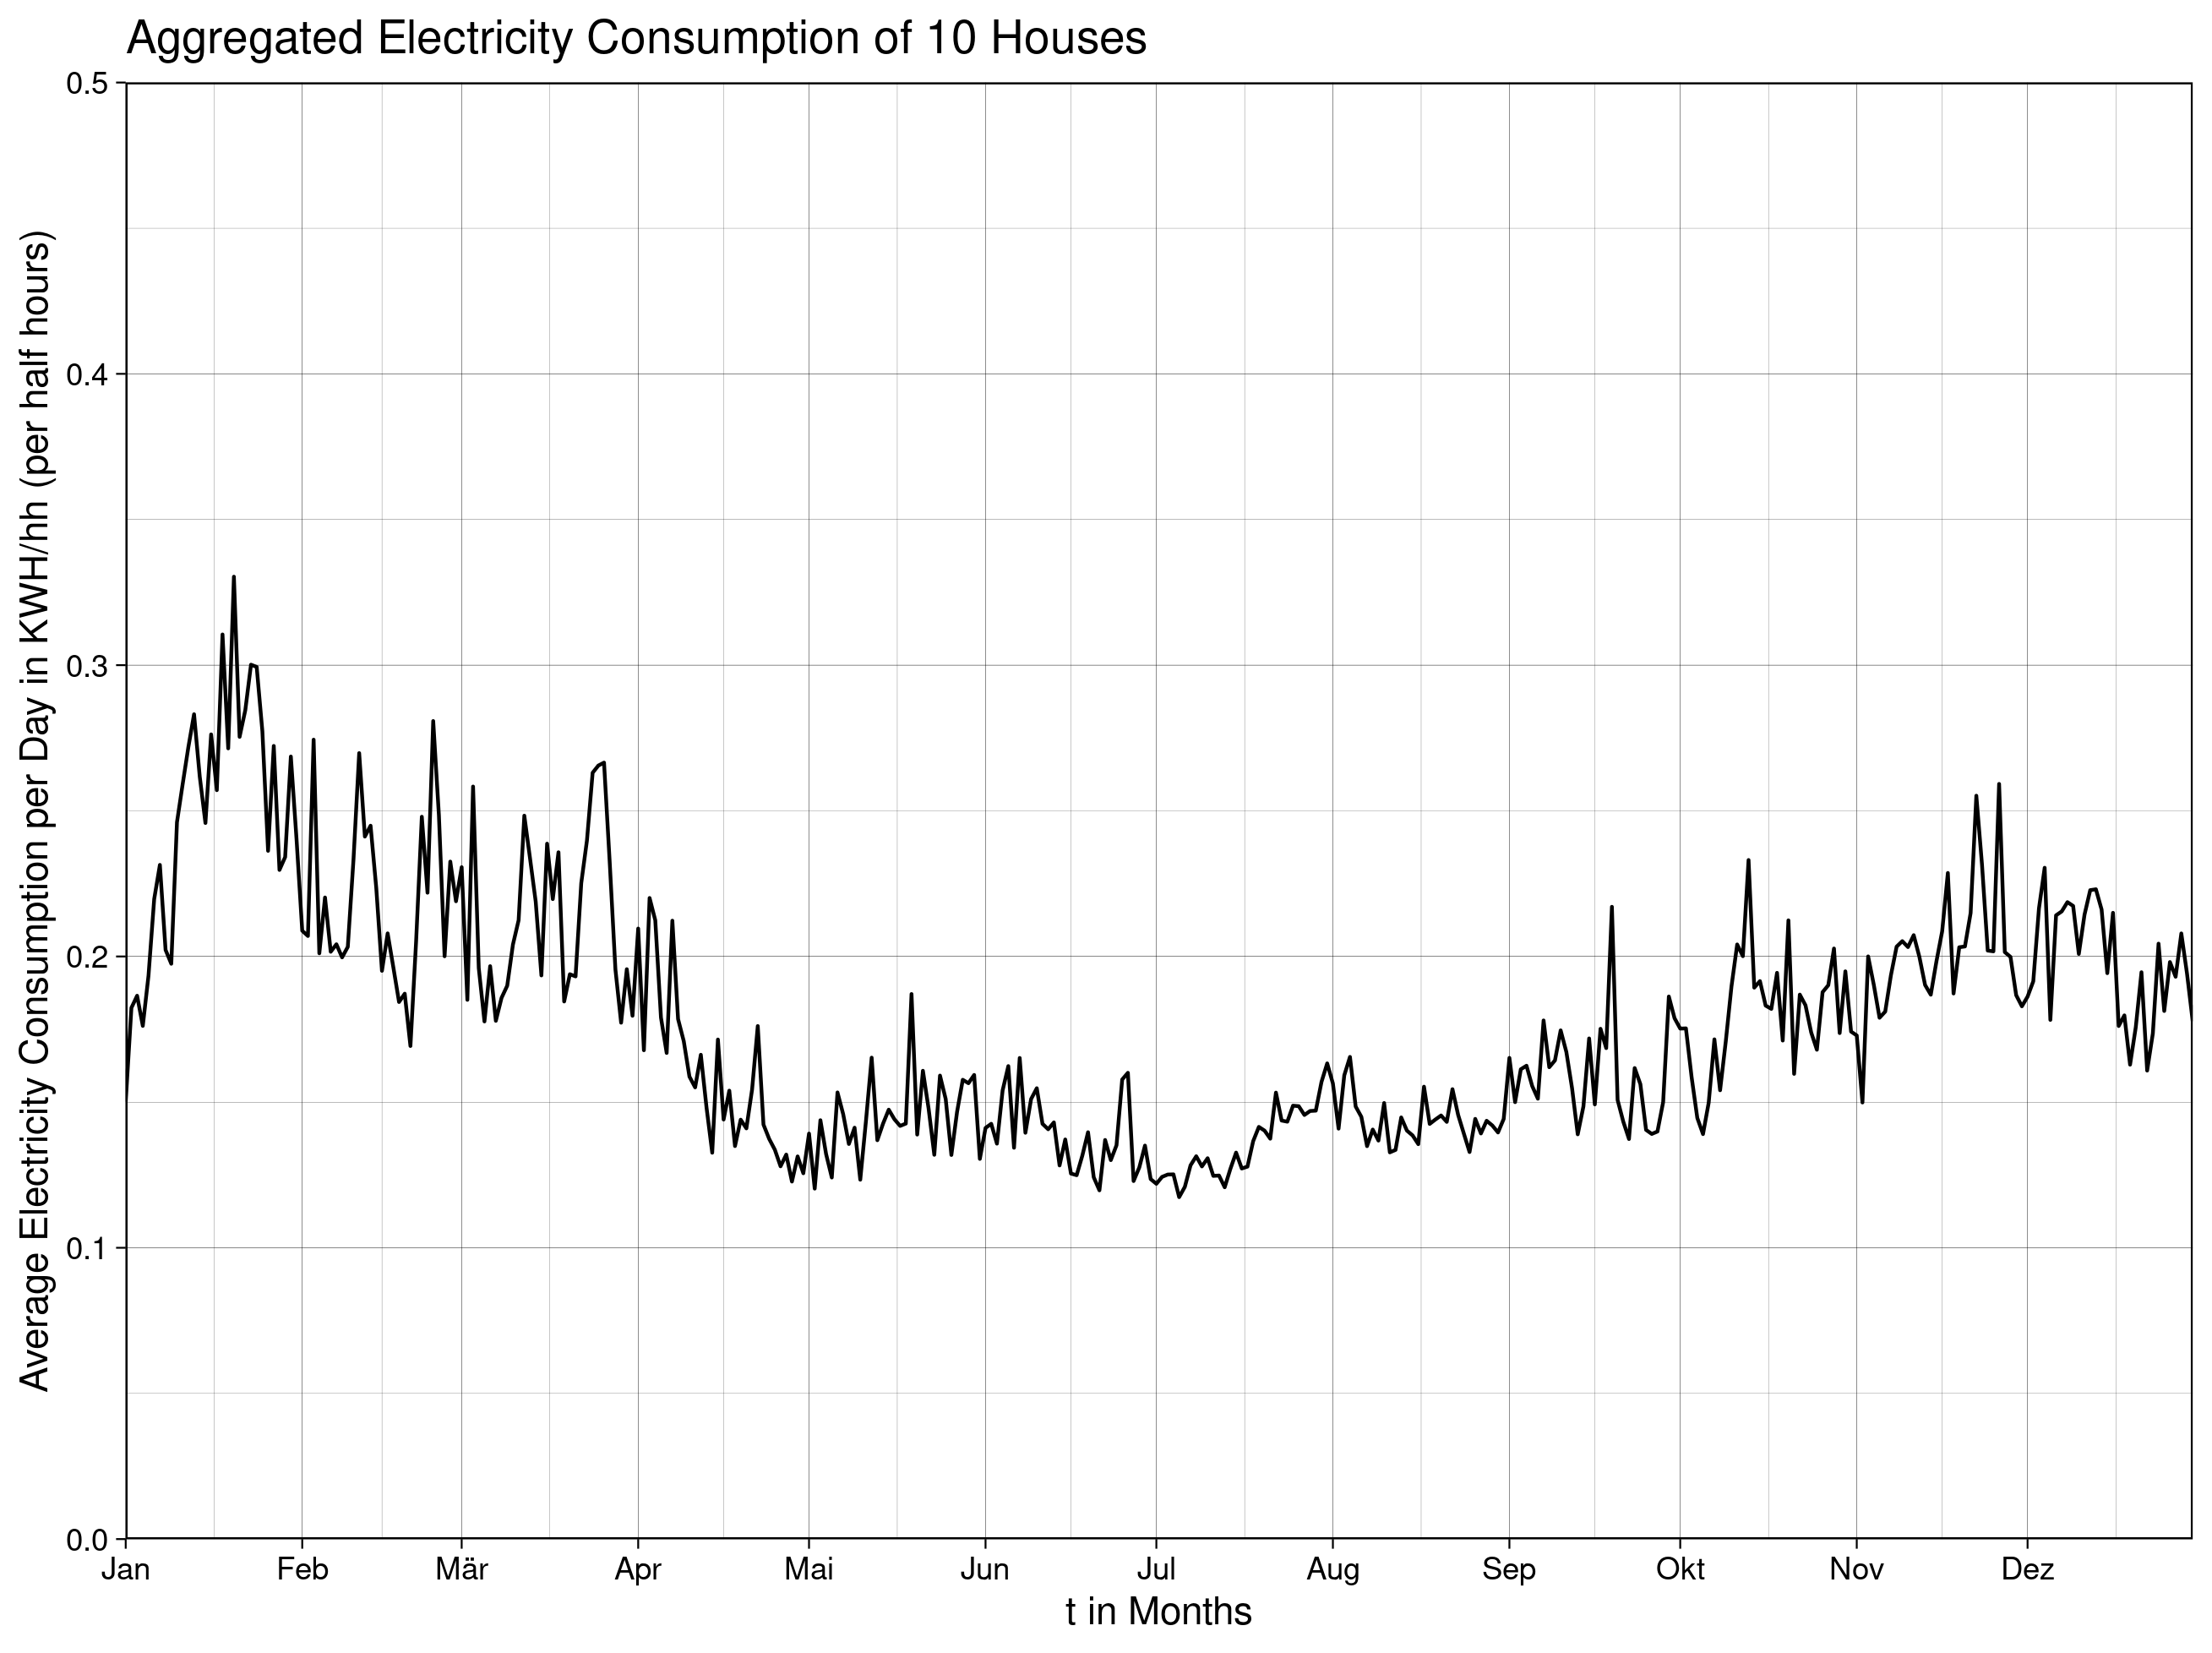
\includegraphics[width=0.85\textwidth]{images/Aggregated Electricity Consumption of 10 Houses.png}
\caption[Aggregated Electricity Consumption of 10 Houses]{}
\label{img:10_Houses}
\end{figure}
\clearpage
}
\afterpage{%
\begin{figure}[!p]
\centering
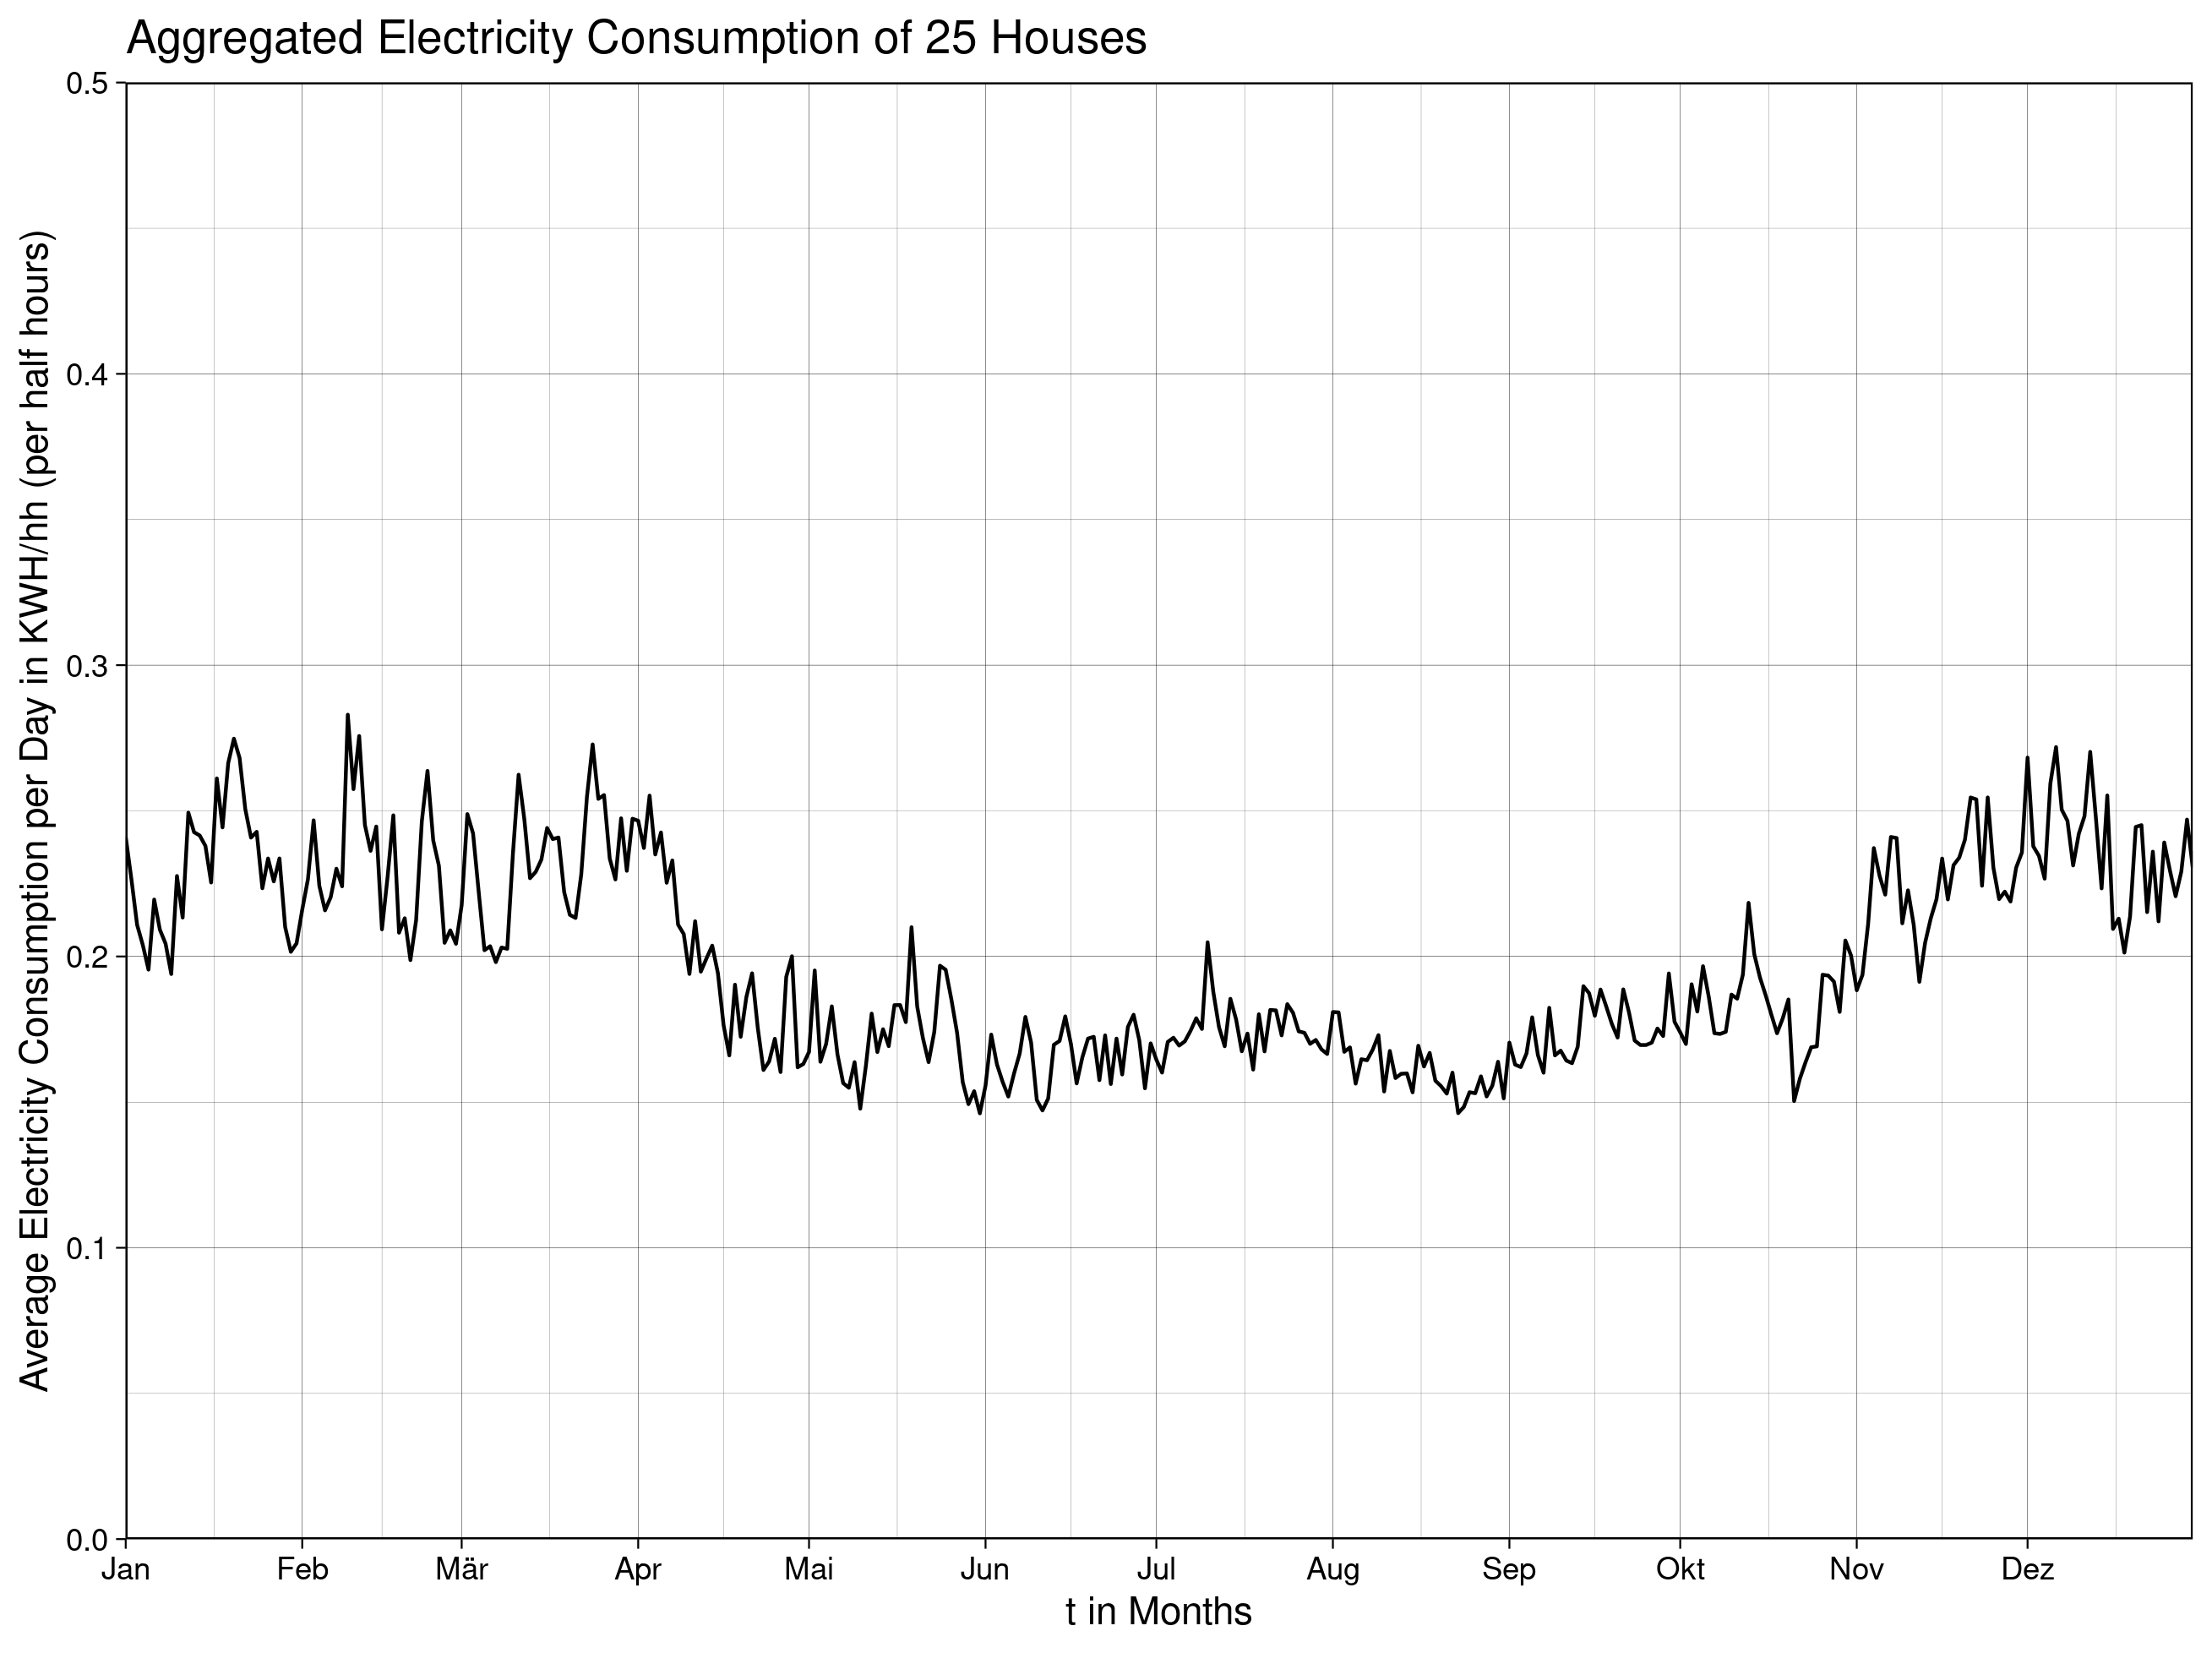
\includegraphics[width=0.85\textwidth]{images/Aggregated Electricity Consumption of 25 Houses.png}
\caption[Aggregated Electricity Consumption of 25 Houses]{}
\label{img:25_Houses}
\end{figure}
\begin{figure}[!p]
\centering
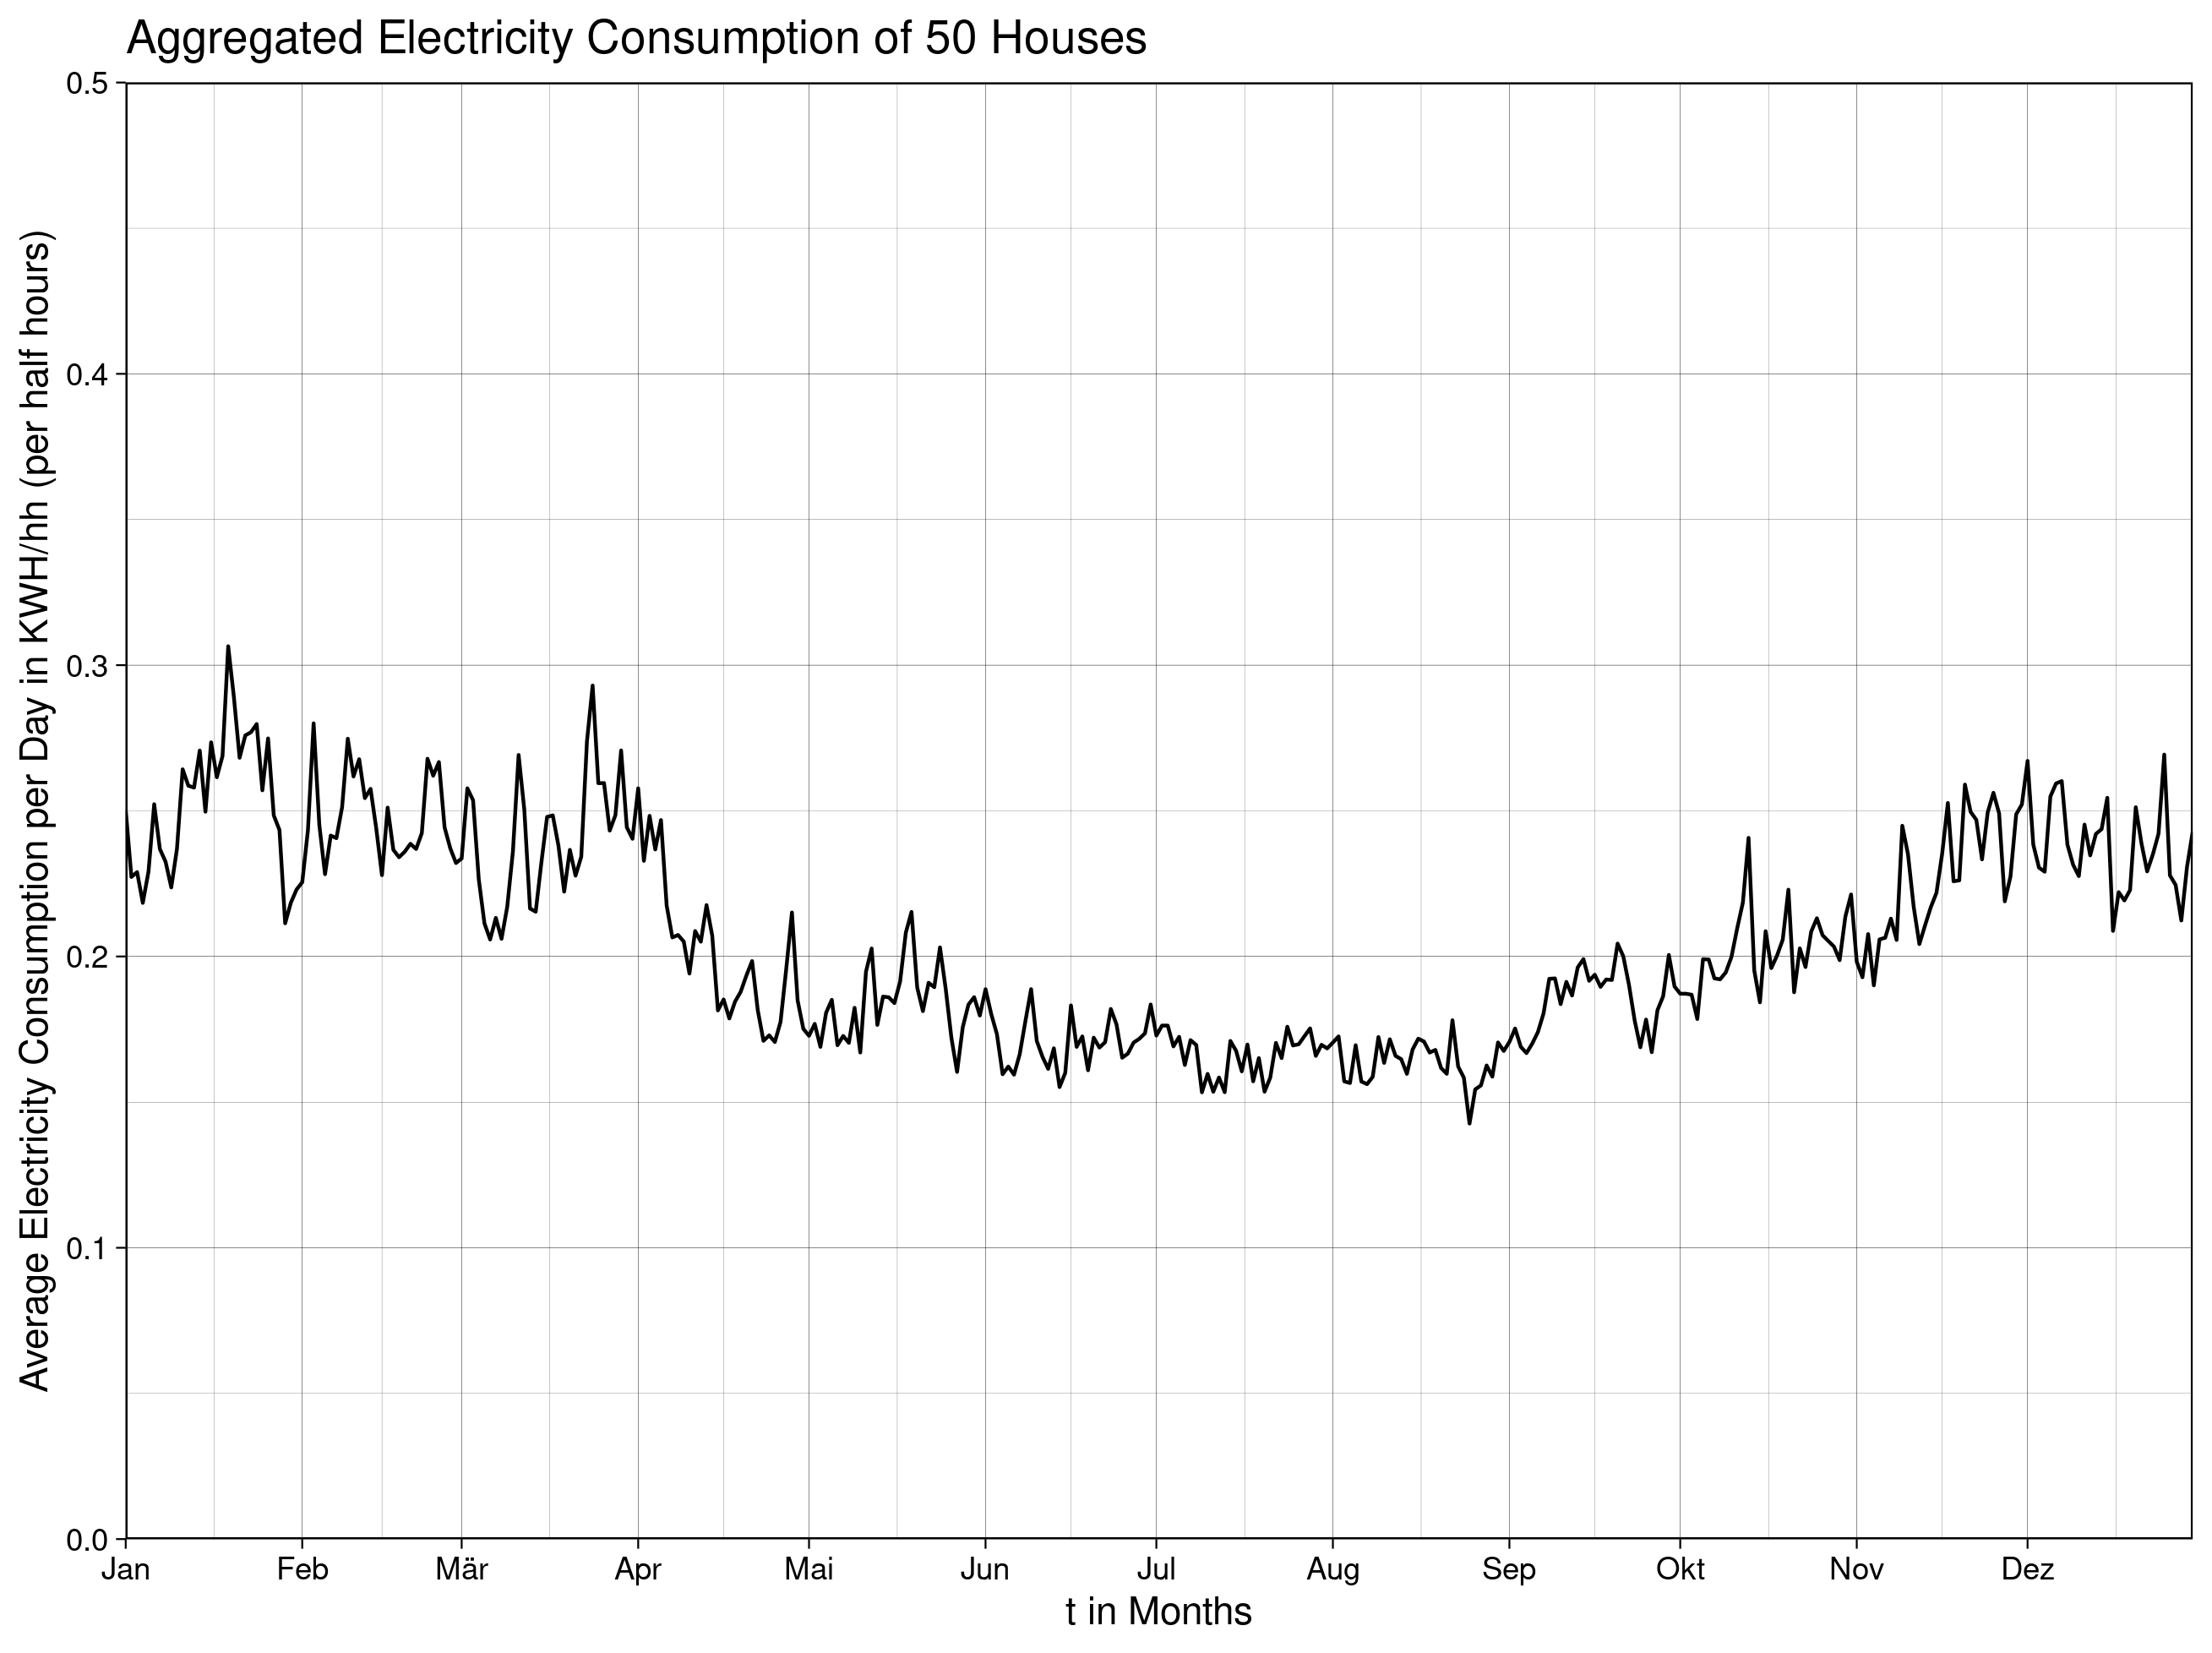
\includegraphics[width=0.85\textwidth]{images/Aggregated Electricity Consumption of 50 Houses.png}
\caption[Aggregated Electricity Consumption of 50 Houses]{}
\label{img:50_Houses}
\end{figure}
\clearpage
}
\afterpage{%
\begin{figure}[!p]
\centering
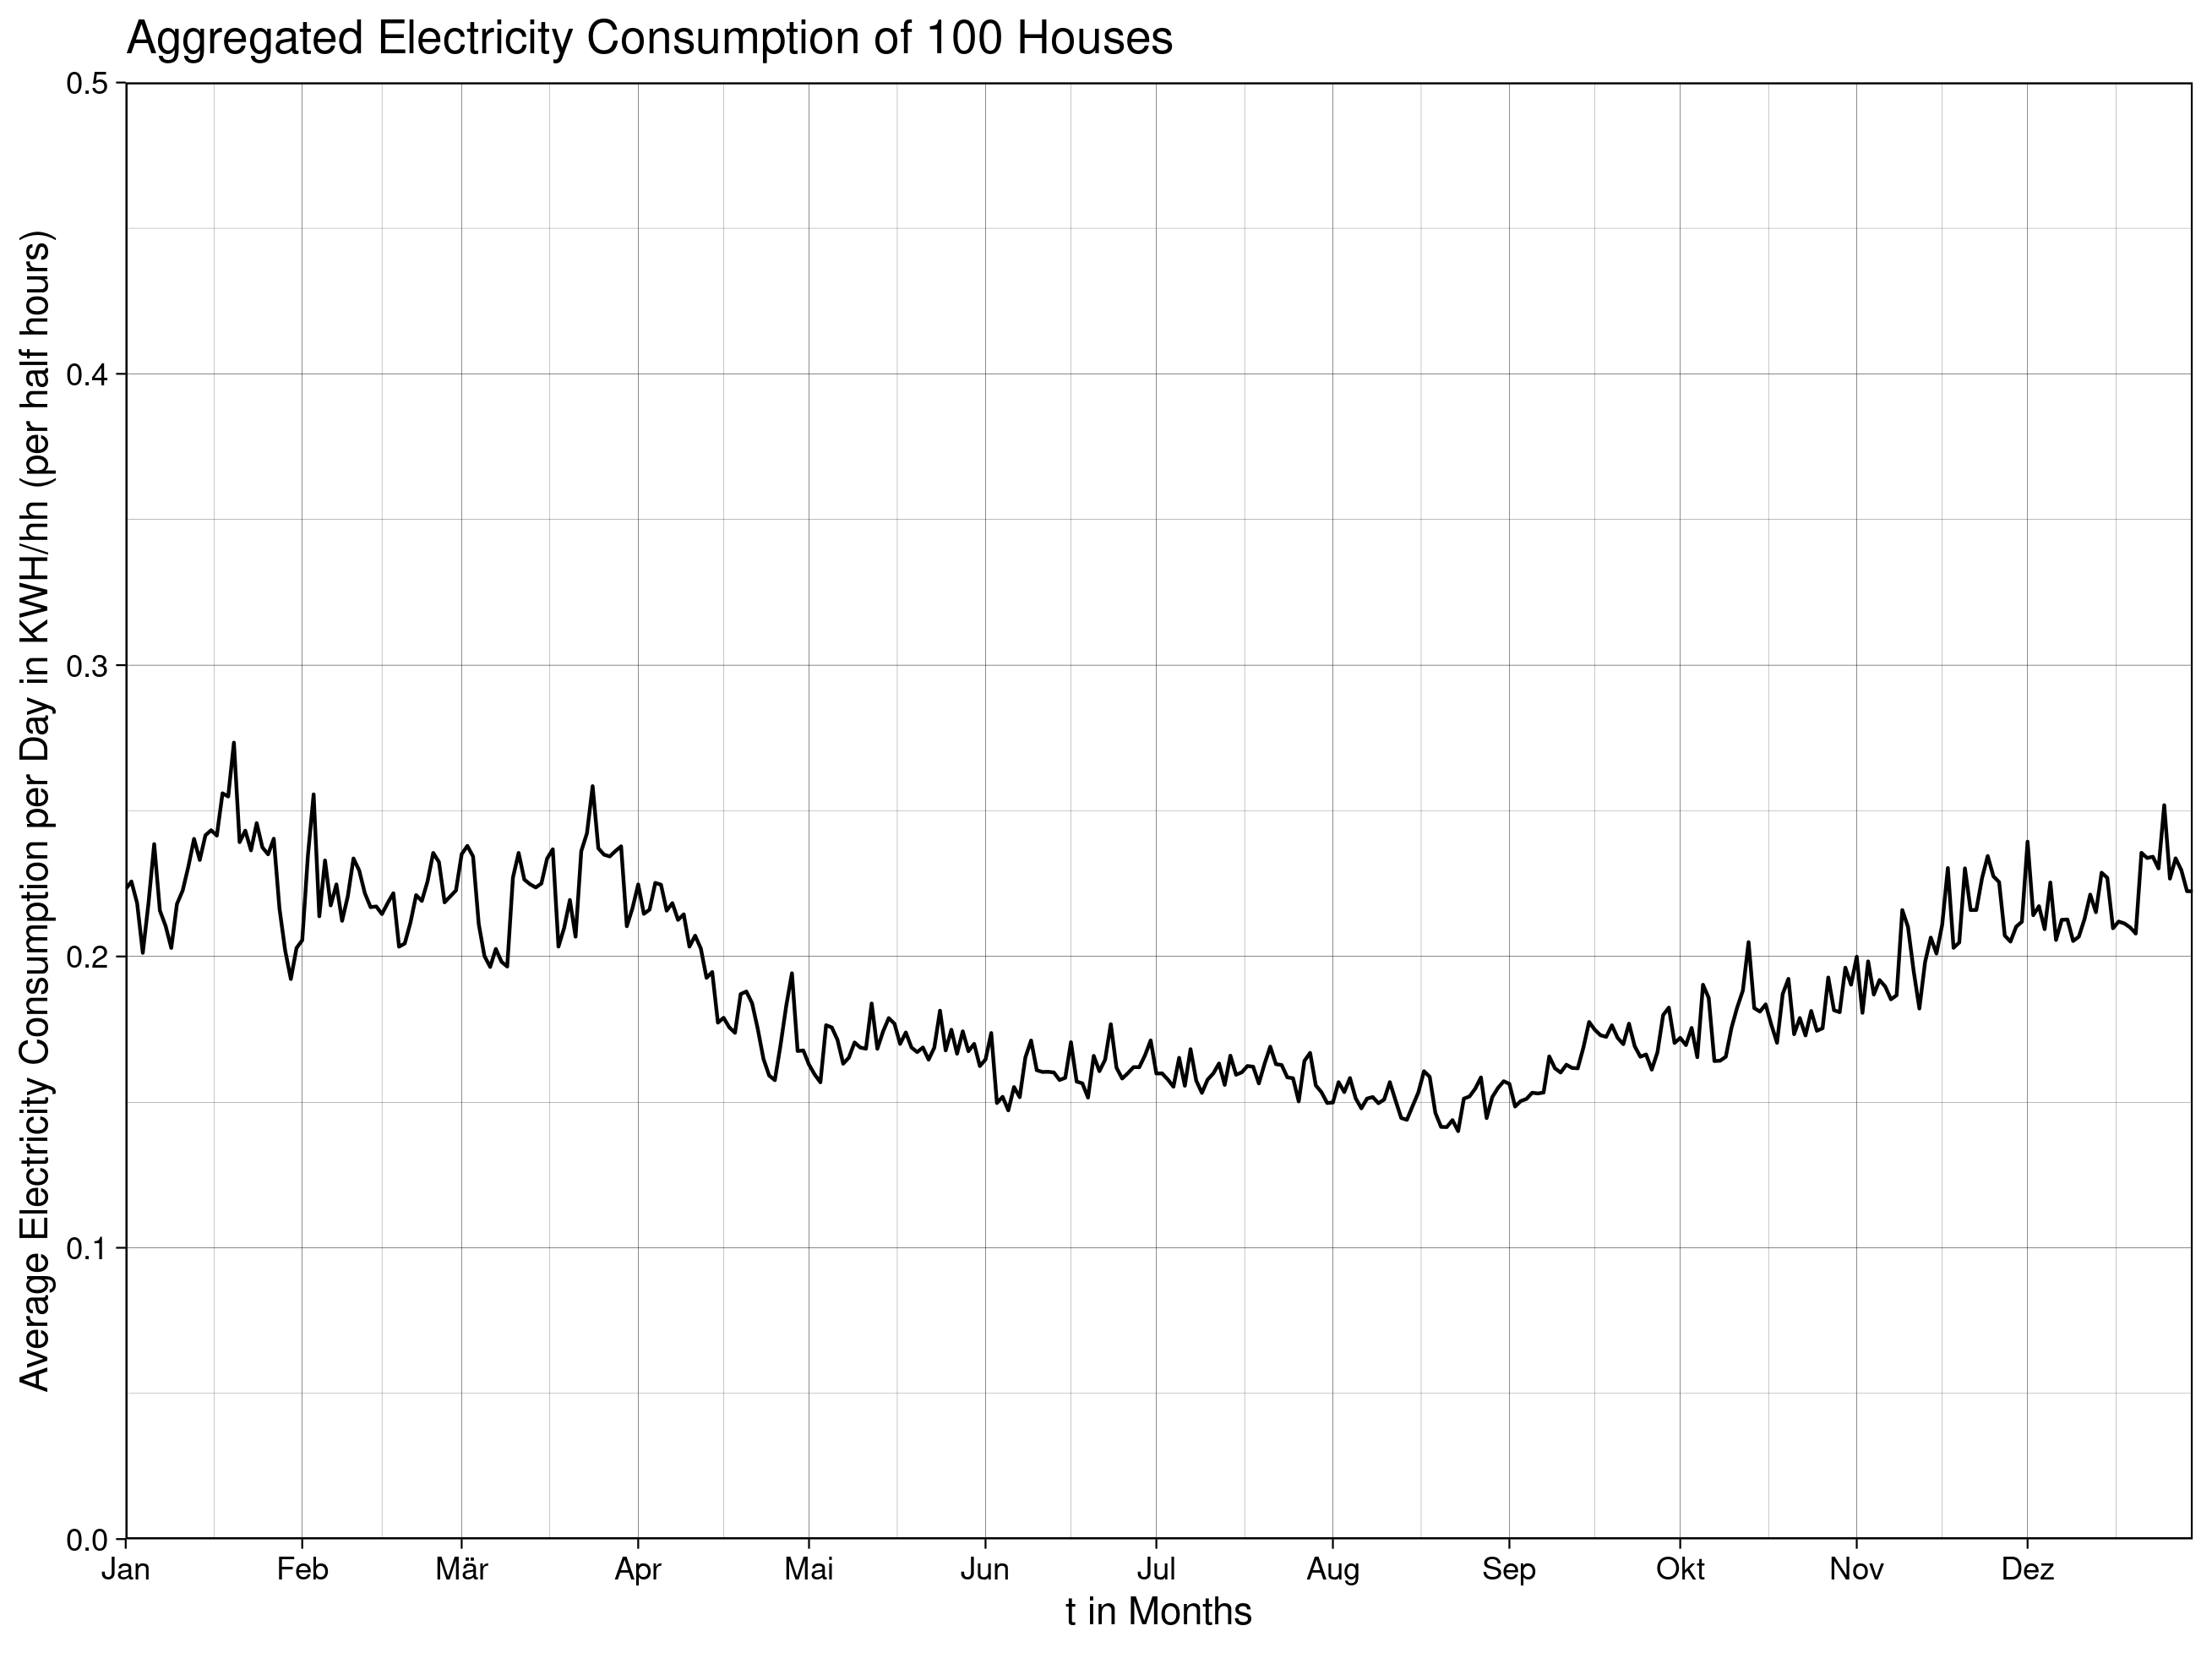
\includegraphics[width=0.85\textwidth]{images/Aggregated Electricity Consumption of 100 Houses.png}
\caption[Aggregated Electricity Consumption of 100 Houses]{}
\label{img:100_Houses}
\end{figure}
\begin{figure}[!p]
\centering
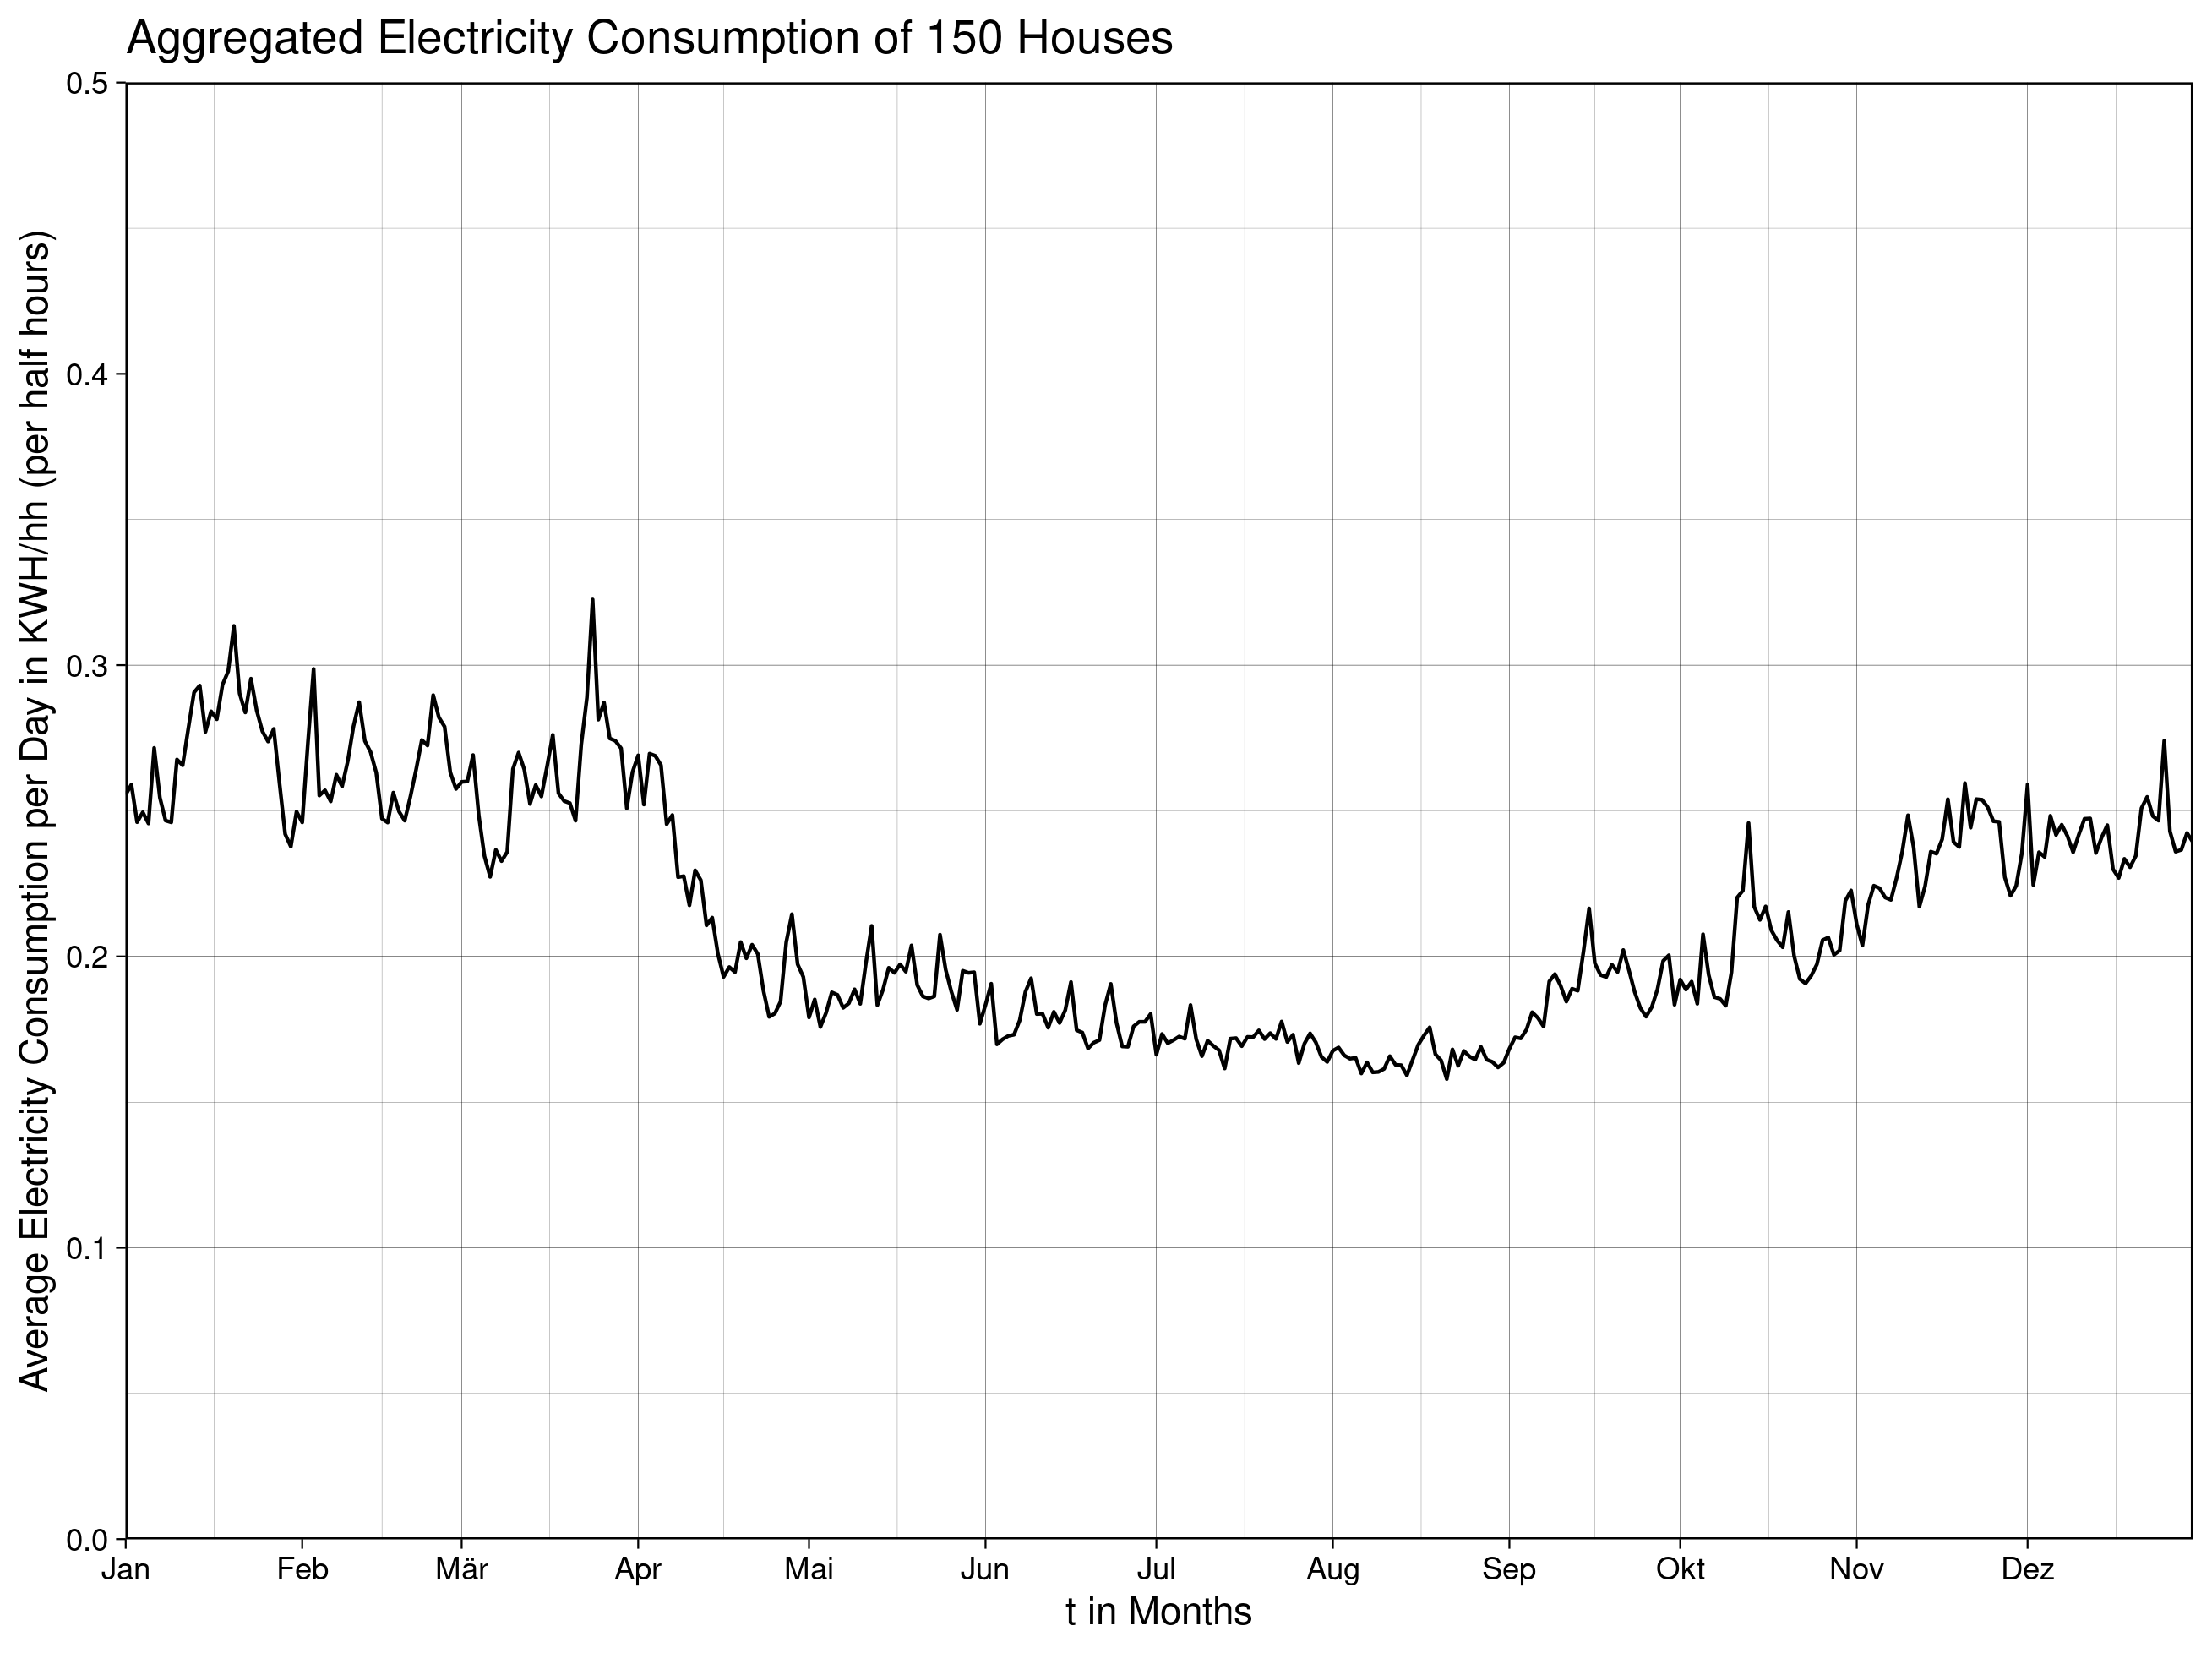
\includegraphics[width=0.85\textwidth]{images/Aggregated Electricity Consumption of 150 Houses.png}
\caption[Aggregated Electricity Consumption of 150 Houses]{}
\label{img:150_houses}
\end{figure}
\clearpage
}

\afterpage{%
\begin{figure}[!p]
\centering
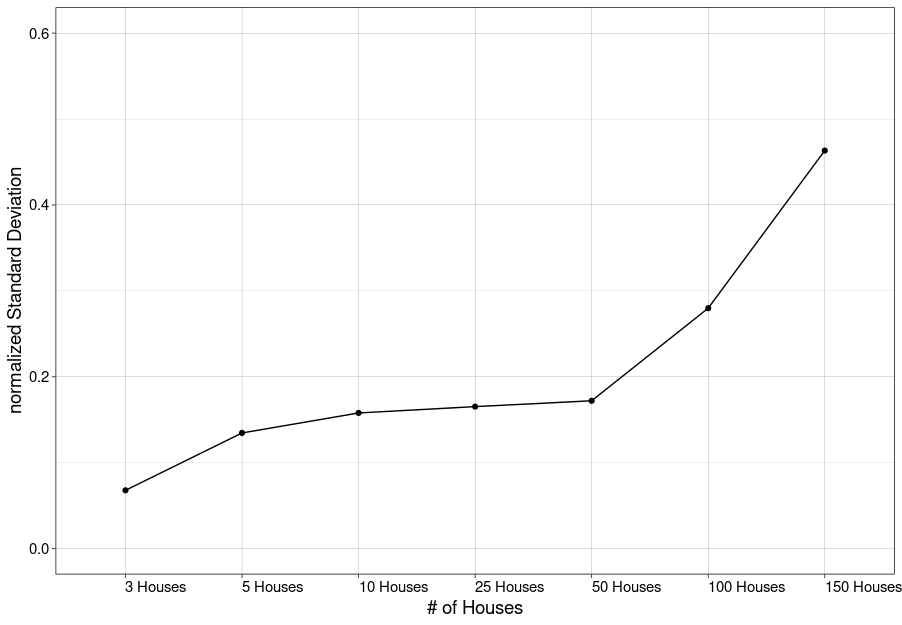
\includegraphics[width=0.85\textwidth]{images/standard_dev_test1.png}
\caption[Standard Deviation of yearlong Experiment]{}
\label{img:SD_year}
\end{figure}
\clearpage
}


\chapter{Experiments}
\label{sec:evaluation}

% Zu jeder Arbeit in unserem Bereich gehört eine Leistungsbewertung. Aus
% diesem Kapitel sollte hervorgehen, welche Methoden angewandt worden,
% die Leistungsfähigkeit zu bewerten und welche Ergabnisse dabei erzielt
% wurden. Wichtig ist es, dem Leser nicht nur ein paar Zahlen
% hinzustellen, sondern auch eine Diskussion der Ergebnisse
% vorzunehmen. Es wird empfohlen zunächst die eigenen Erwartungen
% bezüglich der Ergebnisse zu erläutern und anschließend eventuell
% festgestellte Abweichungen zu erklären.


%statistical analysis and signal processing are being increasingly applied to private data obtained from individuals
The DC network from chapter 3 ensures anonymity of user data in a smart grid. It is impossible for an electricity provider to obtain the individual electricity consumption of a user without performing aggressive attacks. But this criterion alone is insufficient. In chapter two, it was described that 52 different household appliances could be correctly identified from the aggregated electricity consumption of two houses with a accuracy of 55 percent a measurement interval of 1 hour. Accordingly, it is still possible to draw conclusions about individual electricity consumption or about the use of household appliances from different households from an aggregated result. In addition, the measurement interval in the German smart grid is much more frequent and amounts to 15 minutes. To make an analysis over the aggregated result impossible, the DC network must have a minimum number of participants. For this purpose, an experimental analysis was performed in the master thesis to be able to make a statement about the minimum number of participants in a DC network. When researching the information content of aggregated data, only sparse information and no common metric could be found. In particular, of interest is: How much electricity consumption from individual households needs to be aggregated so that certain characteristics, such as the use of individual household appliances, can no longer be analyzed from the results? In this chapter, the experiment investigates from how many participants in the DC network it can be said with certainty that it is no longer possible to draw conclusions about individual users from the result. For this purpose, the assumption and the structure of the experiment and its execution will be described first. Afterwards the results of the experiment are considered and analyzed.
\\
\\
\textbf{Assumption}
\\
\\
The goal of the experiment is that no inferences can be drawn from the result of the aggregated electricity consumption. This includes that no persons can be deanonymized from the result or that no household appliances can be identified from the result. There is no metric that can measure anonymity from electricity consumption, but there are metrics that can measure the information content of electricity consumption. The assumption is therefore that if the information content from the aggregated result of electricity consumption is low, then no conclusions can be drawn about households or household appliances.
\\
\\
\textbf{Experimental Setup}
\\
\\
Ref[relative entropy] described which metrics can calculate the information content of aggregated electricity consumptions. For the experiment, a different procedure was chosen. Electricity consumptions from the London Smart Meter dataset were used. In the dataset, the electricity consumption of 5,567 different households between 2011 and 2014 was recorded with measurement intervals of 30 minutes each. In the experiment, n houses were selected and their electricity consumptions were aggregated for each time point. From the aggregated result, the standard deviation for each individual timestamp was calculated and compared to the individual electricity consumption of a house at that time. The comparison looks if the electricity consumption of a single house is within the tolerance limit of the aggregated result. The tolerance limit is the following interval (aggregated erg- standard deviation<standard deviation<aggregated erg+ standard deviation).  If the electricity consumption of a house is above or below the tolerance limit at a point in time, then it is assumed that the electricity consumption of the house has a high information content at that point in time and that this information content could be read from the result. For each timestamp, each house is counted individually for how often the individual power consumptions are outside the tolerance limit. In order to perform the experiment, a script was programmed in R, which selects random houses from the London Smart Meter data set. Additionally, we filtered for houses that have readings between 2013 and 2014. For the highest possible precision of the calculation, it was ensured that when a comparison calculation is performed, the timestamp is also correctly identical. In short every 30 minutes measurements in 2013-2014 of a house were compared whether the electricity consumption is above or below the tolerance limit of the aggregated results of N houses. For each calculation, the number of times the values are outside the tolerance limit is counted. This experiment was repeated with different N sizes to analyze how strong the effects of the information content in the aggregated result are measurable.
\\
\\
\textbf{Results}
\\
\\
Figure 5.1 - 5.8 show the results of the experimental tests. Experiments were conducted with 2, 3, 5, 10, 25, 50, 100 and 150 random chosen houses per group, whose electricity consumptions were aggregated and the experiments were repeated 2 times. On the X-axis the time in months can be read. On the Y-axis, the average daily electricity consumption within half an hour of a house can be read. If the figure is considered, it can be seen that in the experiments with little aggregated houses (2,3,5,10) more significant variations in the amplitude of the characteristic curves are visible. This can be explained by the fact that in the case of less aggregated houses, individual power consumptions have a greater impact and can therefore have a more significant effect on the overall result. This could be an indication that the information content of a single house can still be determined. As an example, the diagram [ref] with the aggregation group of 2 houses can be viewed. Between the end of March and April there is a noticeable gap and low power consumption in both houses. In London, there were school vacations in 2013 exactly in this period and the assumption is that both households were on vacation in the mentioned period.\\
From 25 - 150 houses the characteristic curves approach the same pattern. The seasons can be clearly recognized. This is directly evident in the house groups 2-10. The fact that the seasons can be recognized so clearly, can be argued indirectly with the fact that a larger house group is observed. This is because individual household appliances no longer stand out clearly and larger patterns of behavior can be recognized, such as the fact that in the winter, people spend more time inside their homes, while in the summer, they spend more time outside. In addition, it is noticeable that the average base load is different in each graph, but converges briskly for larger aggregation groups. 

The average base load can best be viewed in the boxplot diagram by the median. The boxplot diagram almost summarizes the diagrams 5.1 -5.8 with one boxplot each. In conducting the experiments, the preliminary assumption was that with larger aggregations, the result would approach a horizontal constant. The approximation of a constant would be clear evidence that the information content in the result was lost. The experiment cannot prove the prior conjecture. If the results were to converge to a constant at larger aggregations, then the upper quartile and the lower quartile would become narrower at larger aggregation groups. However, this observation cannot be obtained from the boxplot. 
In addition, the number of occurrences that a house's electricity consumption falls outside the REF tolerance range for each timestamp in a year was counted. Figure 5.10 shows the percentage deviation of the tolerance range in the aggregation groups. It can be seen that the percentage deviation is very low for 2 houses and increases sharply for 3 houses and above. The behavior could be observed in both trials of the experiment. One reason for the observation could be that the standard deviation is a measure of the spread of the values of a feature from the average. With so few values, the result of the standard deviation is in many cases larger than the difference of a power consumption to the normalized aggregated result of both houses. Accordingly, almost all values are within the tolerance range. From 3 results onwards, this behavior no longer seems to apply and the number of deviations increases sharply. The number of deviations reaches its highest value in the aggregation group of 10 houses and then the percentage deviation drops sharply. The renewed noticeable increase at 50 houses could not be confirmed in the second experiment and is therefore considered an outlier. The experiment shows that the information content has strongly decreased from an aggregation group of 25 houses and the larger the aggregation group becomes the smaller the counted deviations are outside the tolerance range.
\afterpage{%
\begin{figure}[!p]
\centering
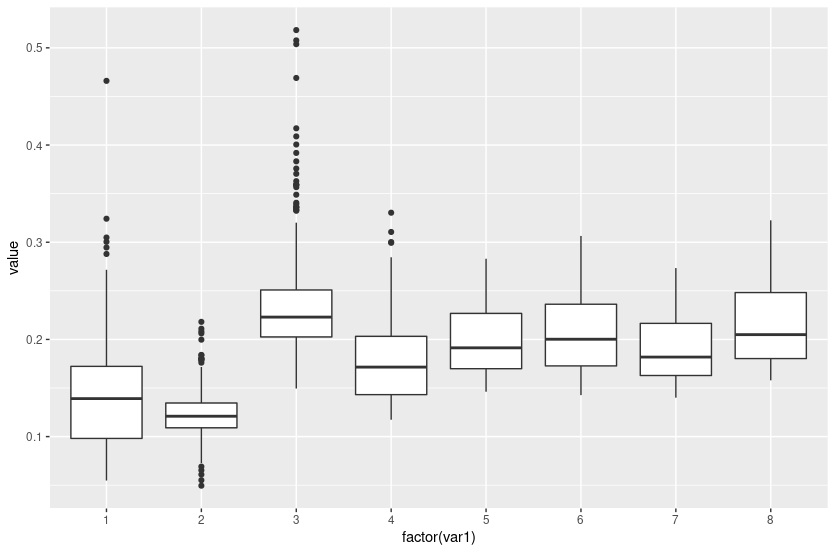
\includegraphics[width=0.85\textwidth]{images/ggplotTest.png}
\caption[Bandbreite Diagramm mit aktivierter Verschlüsselung]{}
\label{img:bytes-e}
\end{figure}
\begin{figure}[!p]
\centering
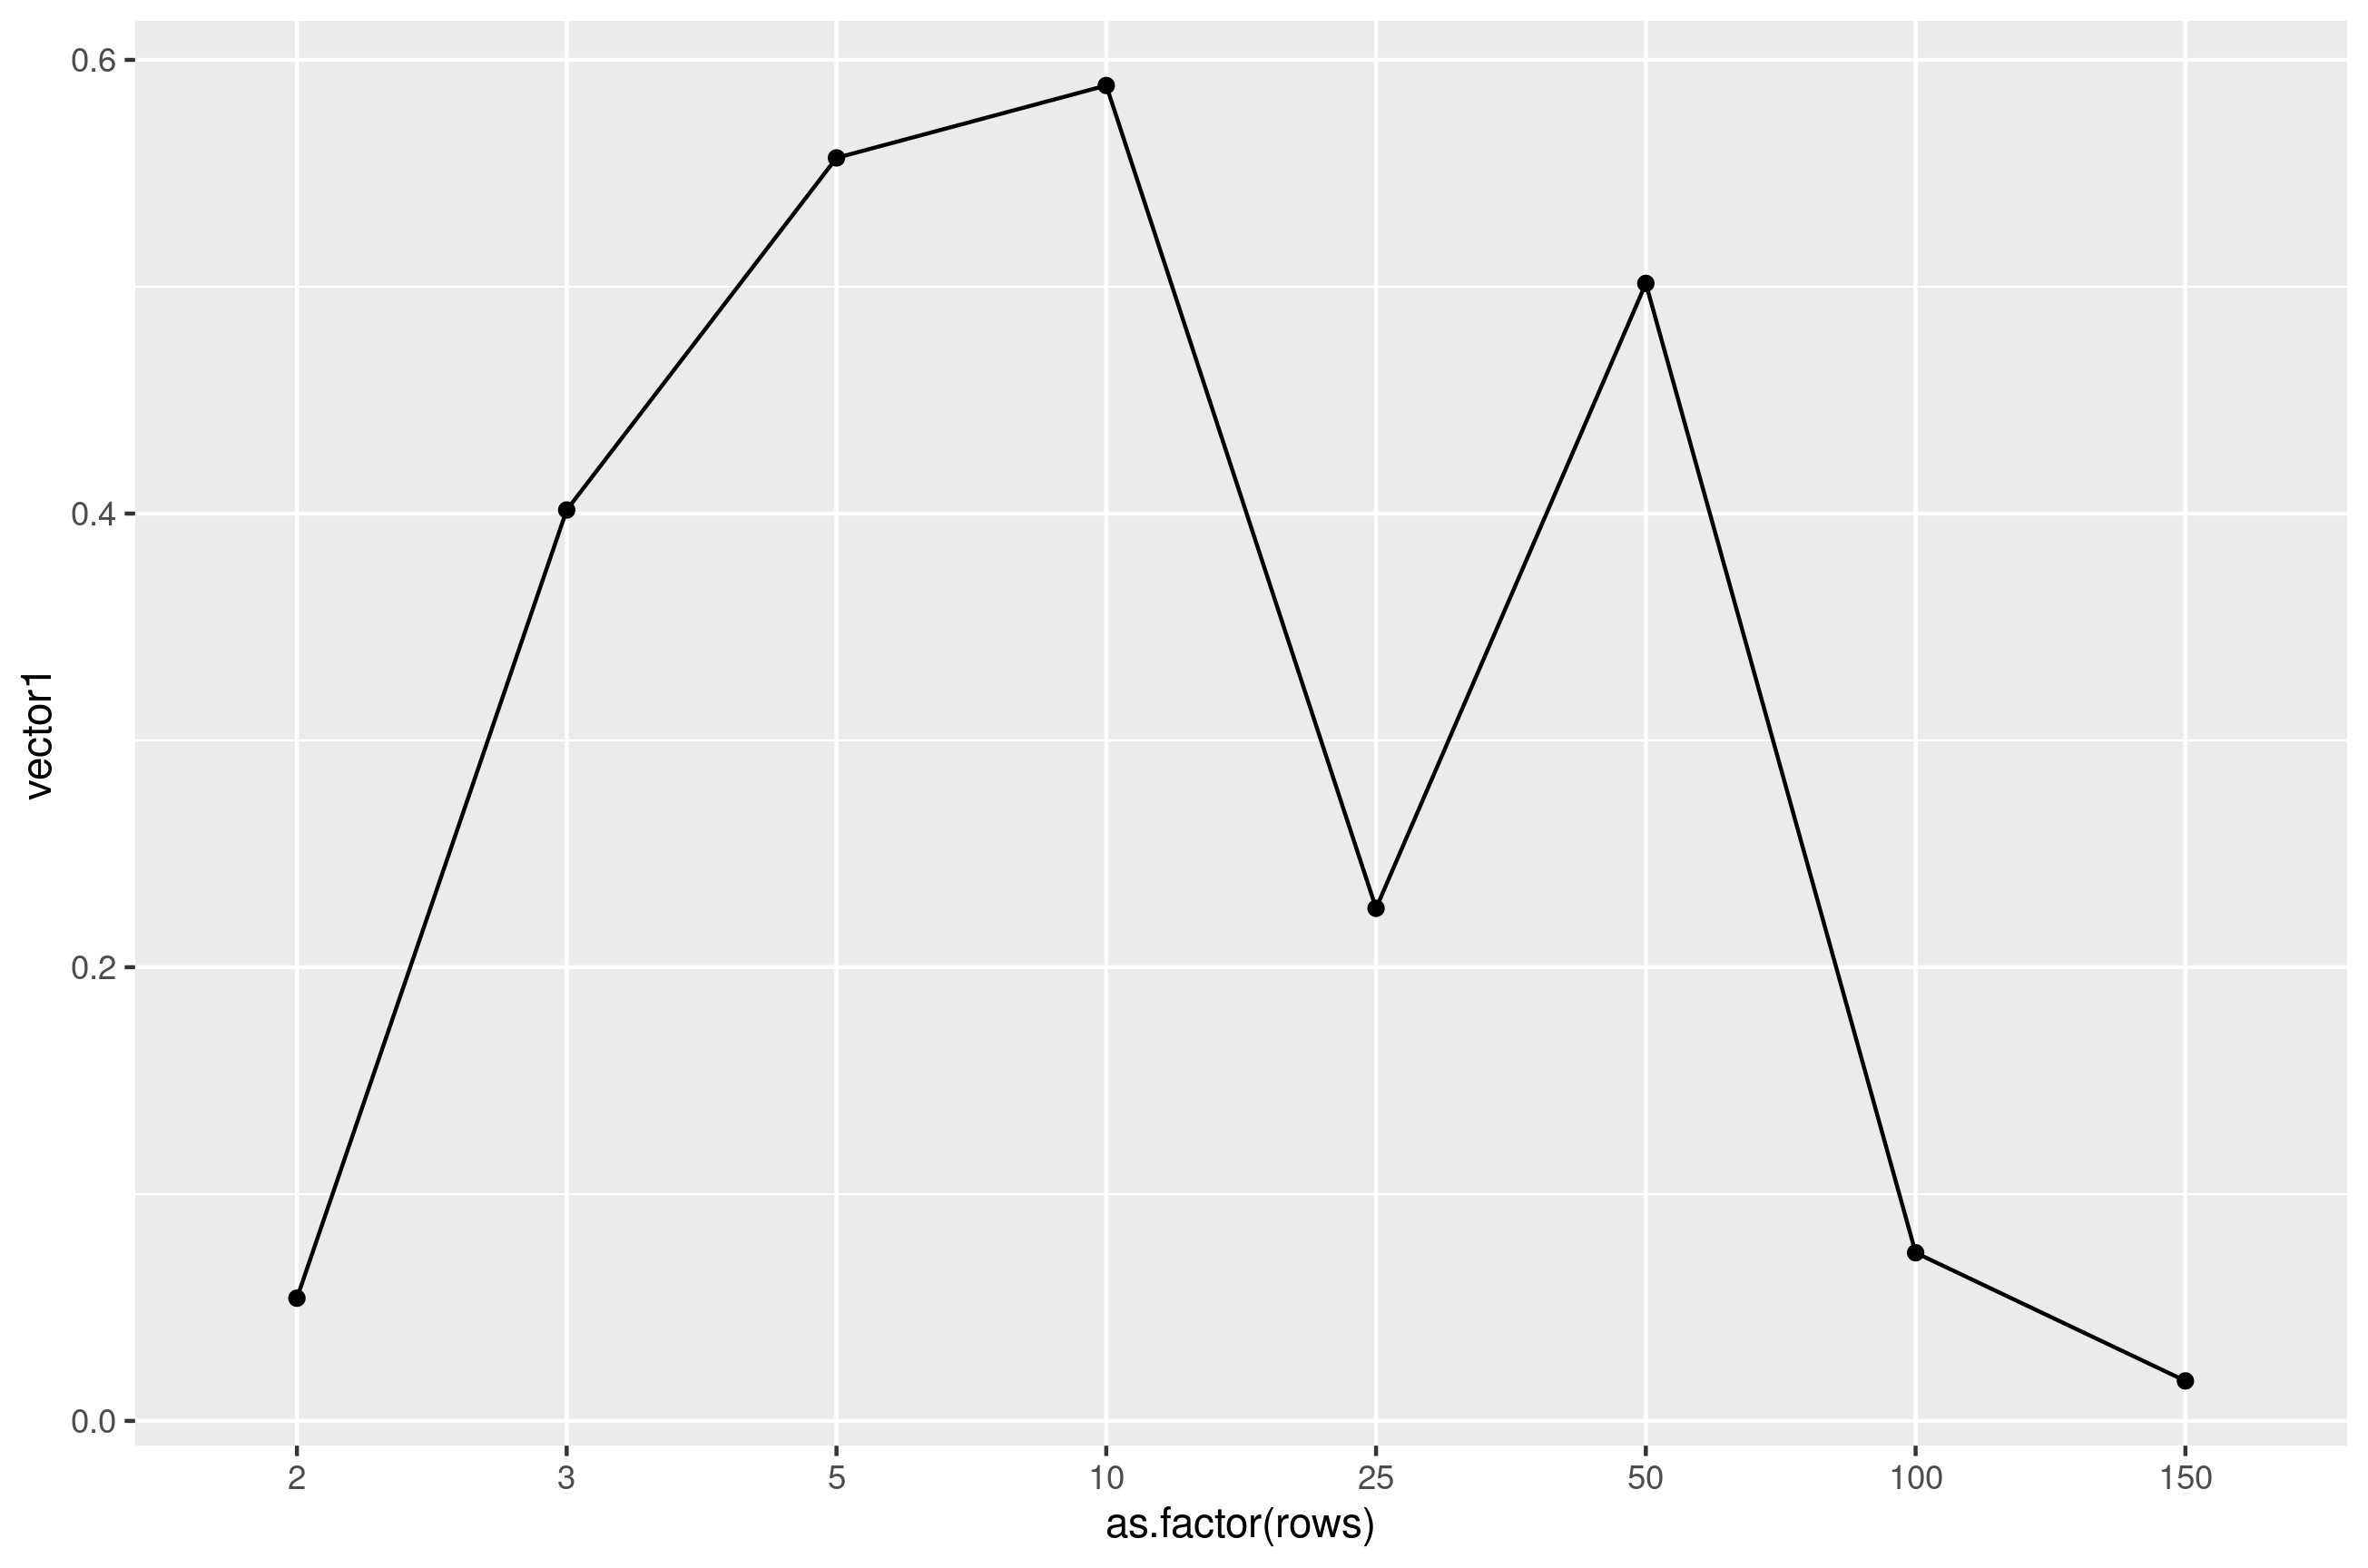
\includegraphics[width=0.85\textwidth]{images/test.png}
\caption[Diagramm der Bandbreite ohne Verschlüsselung]{}
\label{img:bytes-we}
\end{figure}
\clearpage
}

%Nachschauen mit den ferien im april bei 2 häusern
%durchschnittliche Mittelwert(von boxplots)
%ergebnisse der abweichung
%versuche wurden 2 mal wiederholt.

\afterpage{%
\begin{figure}[!p]
\centering
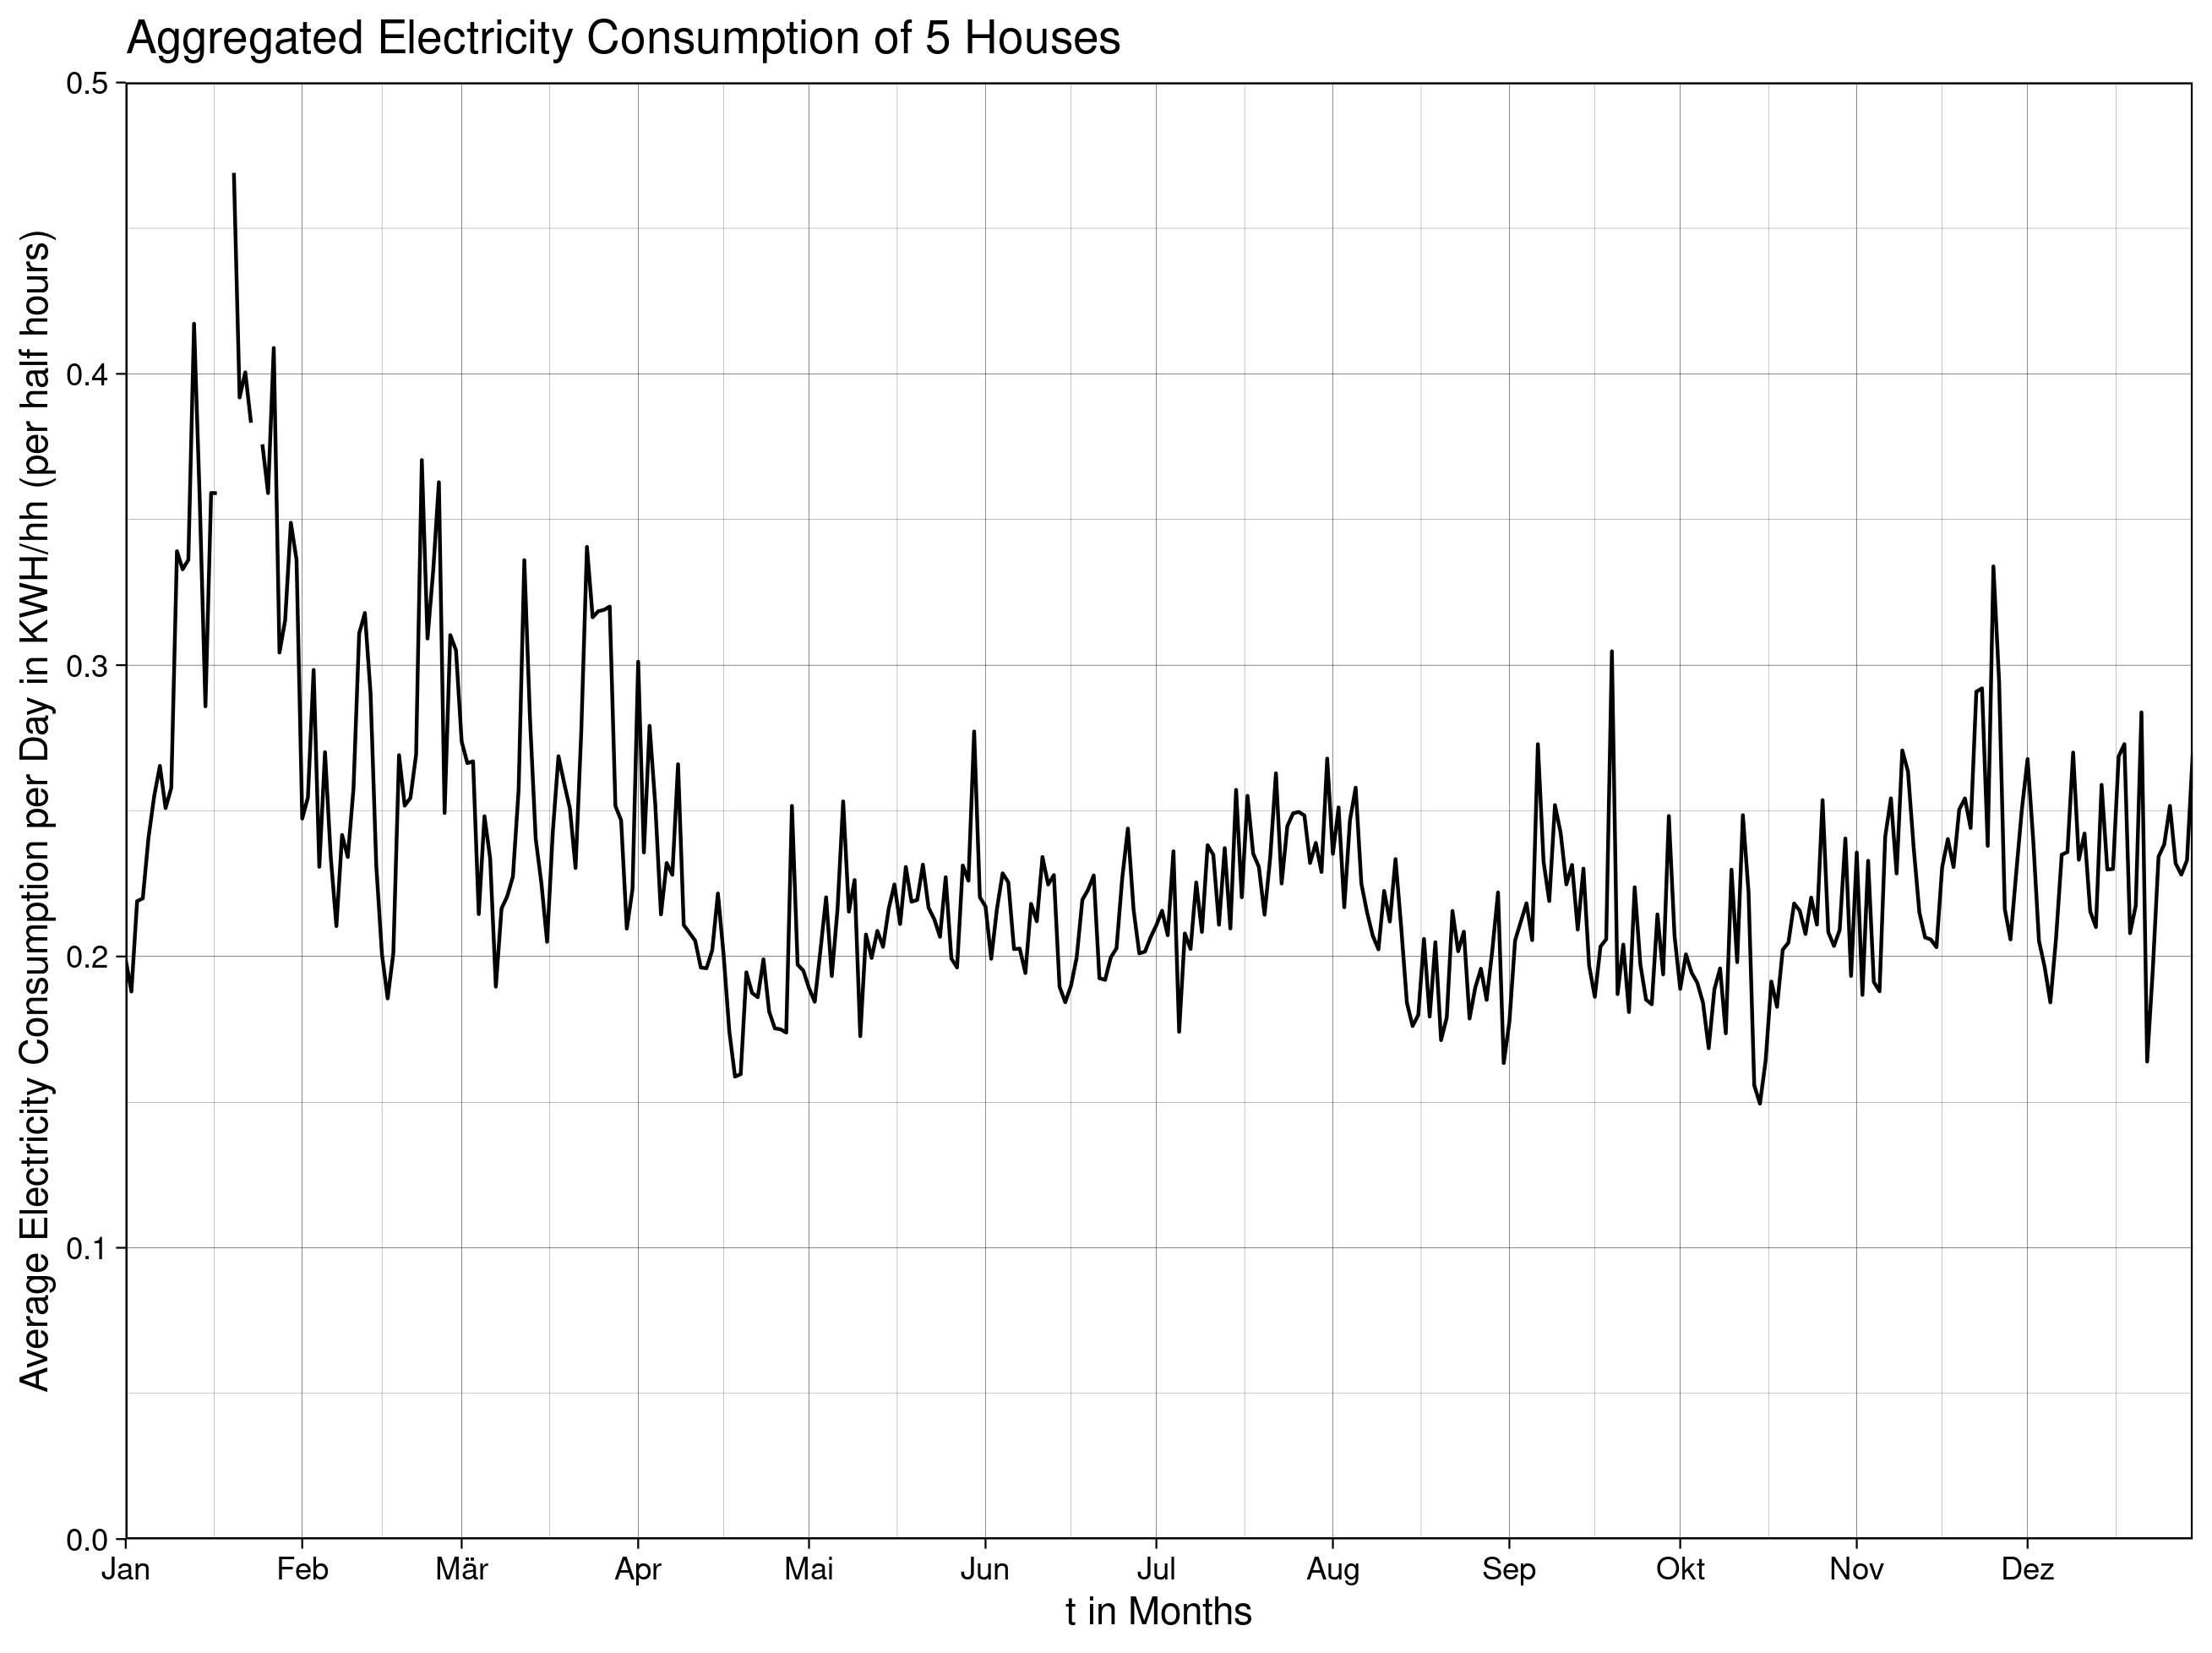
\includegraphics[width=0.85\textwidth]{images/Aggregated Electricity Consumption of 5 Houses.png}
\caption[Bandbreite Diagramm mit aktivierter Verschlüsselung]{}
\label{img:bytes-e}
\end{figure}
\begin{figure}[!p]
\centering
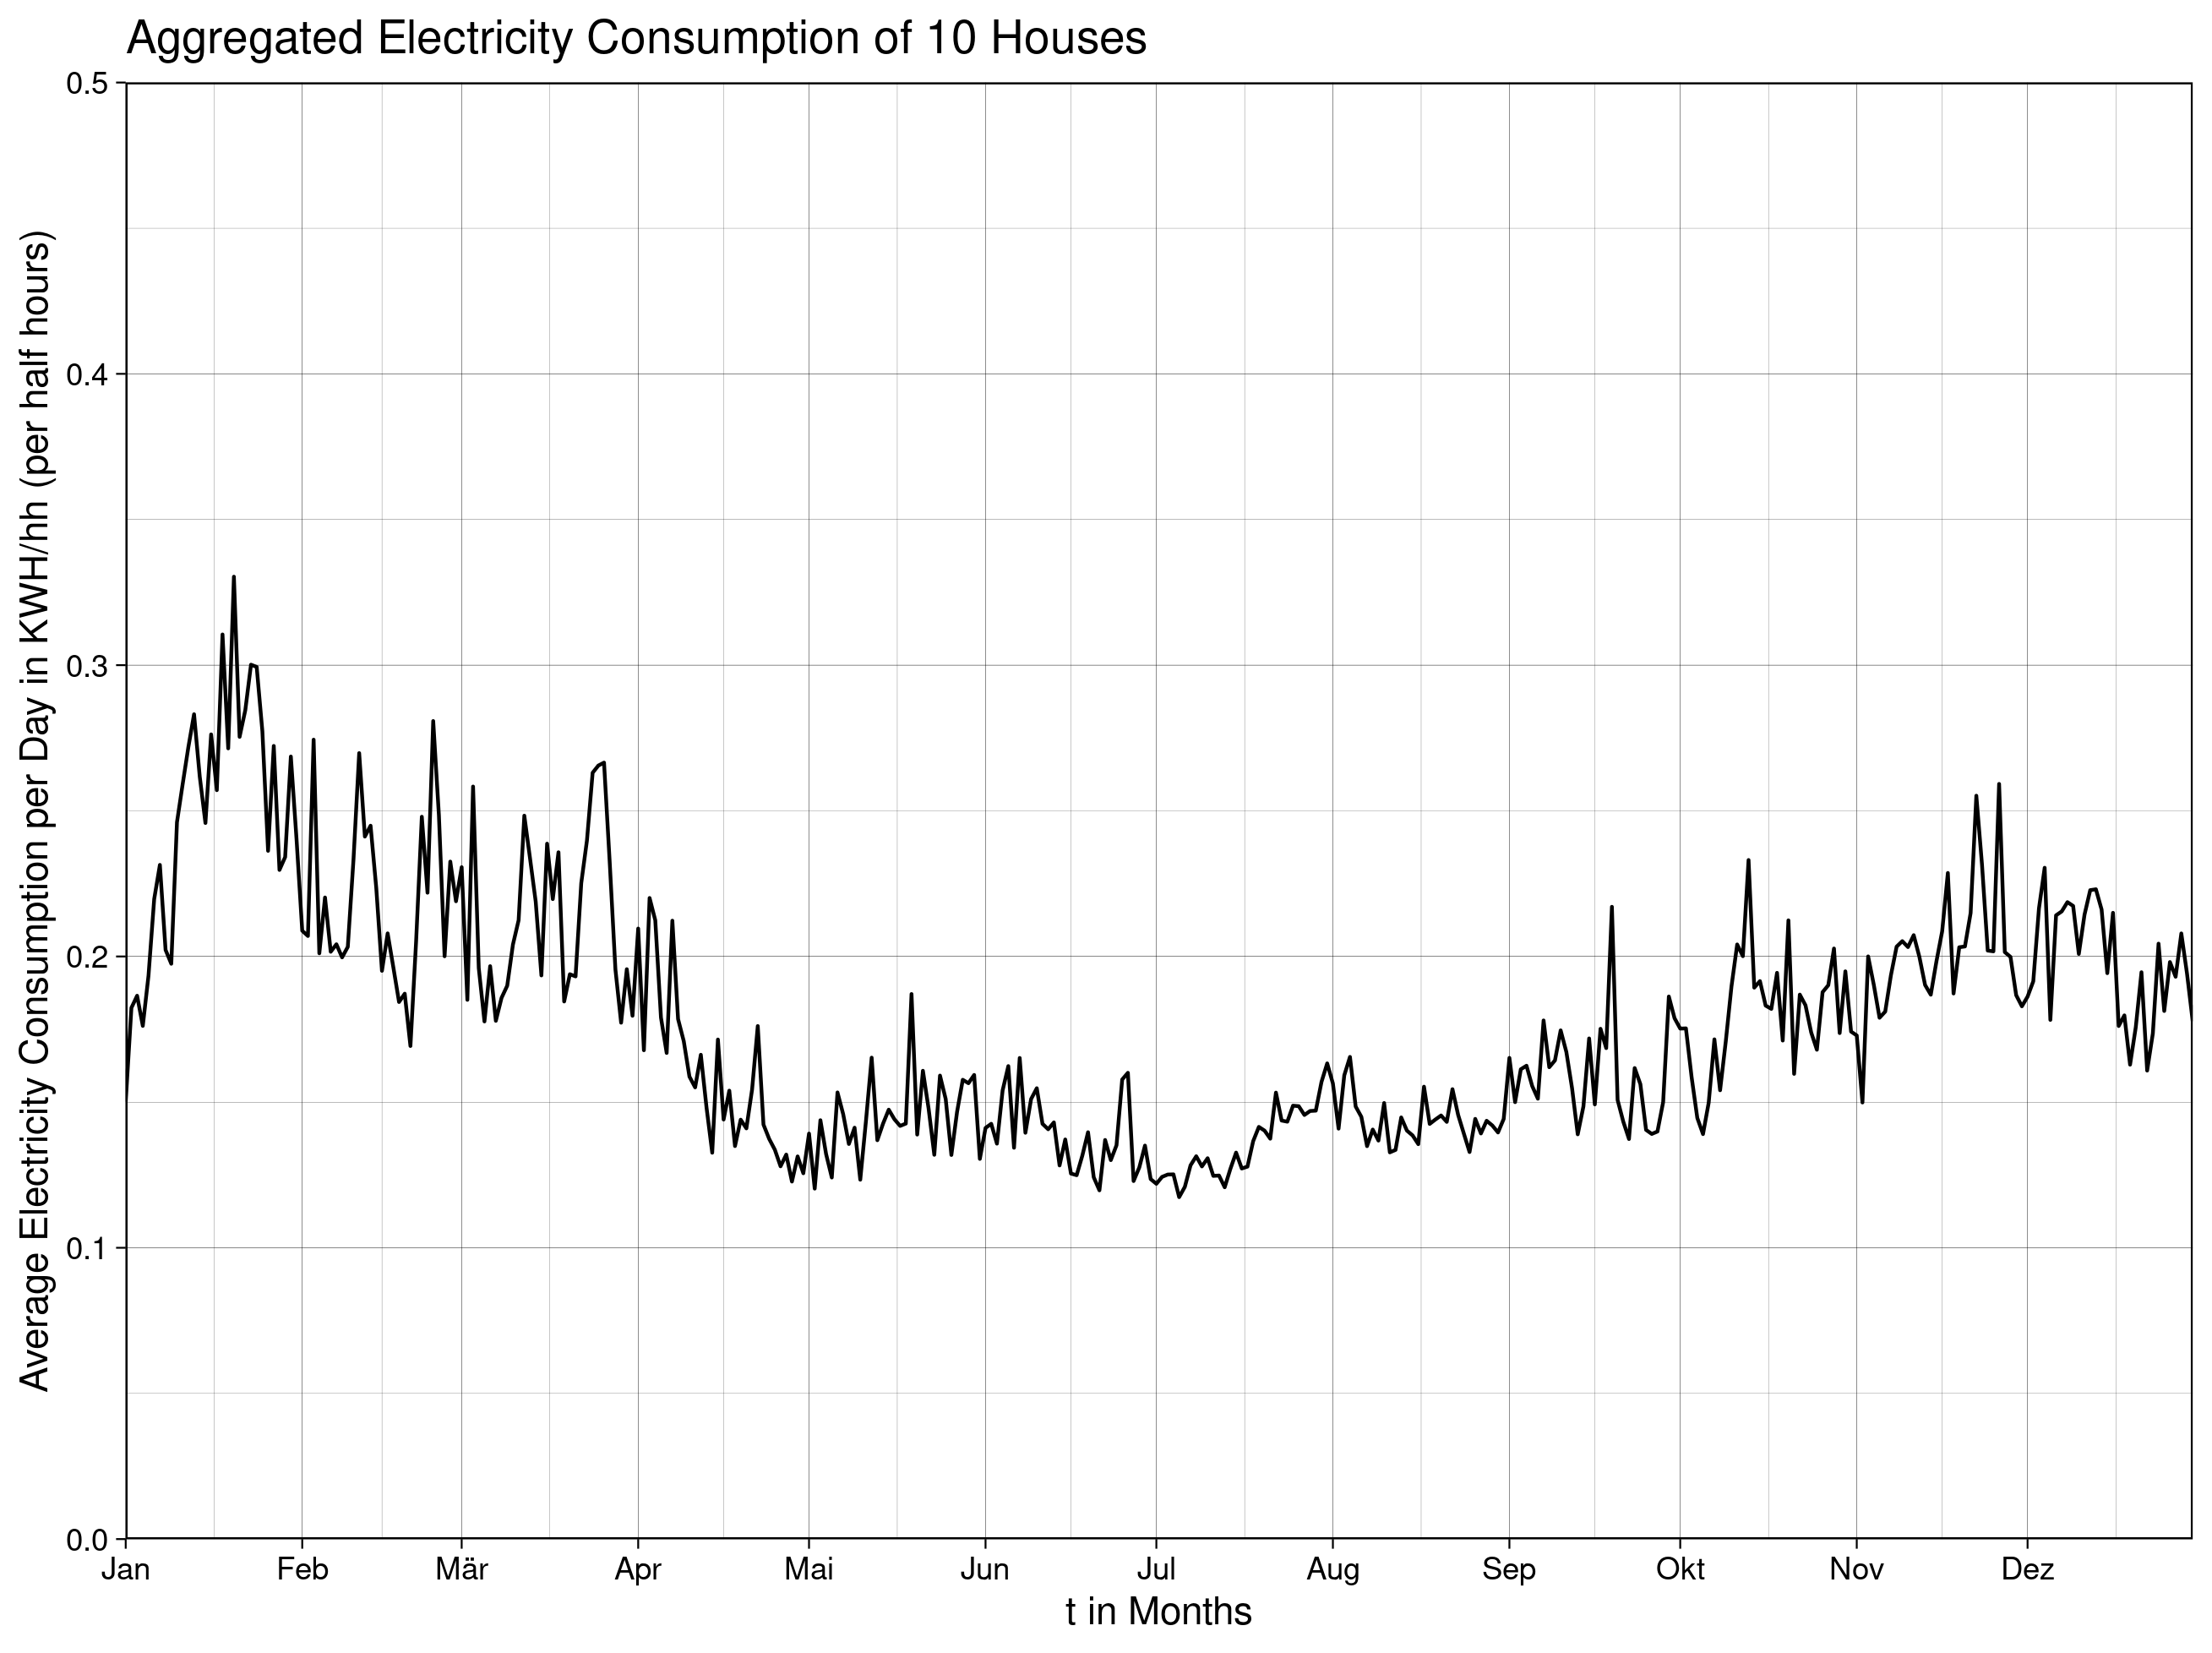
\includegraphics[width=0.85\textwidth]{images/Aggregated Electricity Consumption of 10 Houses.png}
\caption[Diagramm der Bandbreite ohne Verschlüsselung]{}
\label{img:bytes-we}
\end{figure}
\clearpage
}
\afterpage{%
\begin{figure}[!p]
\centering
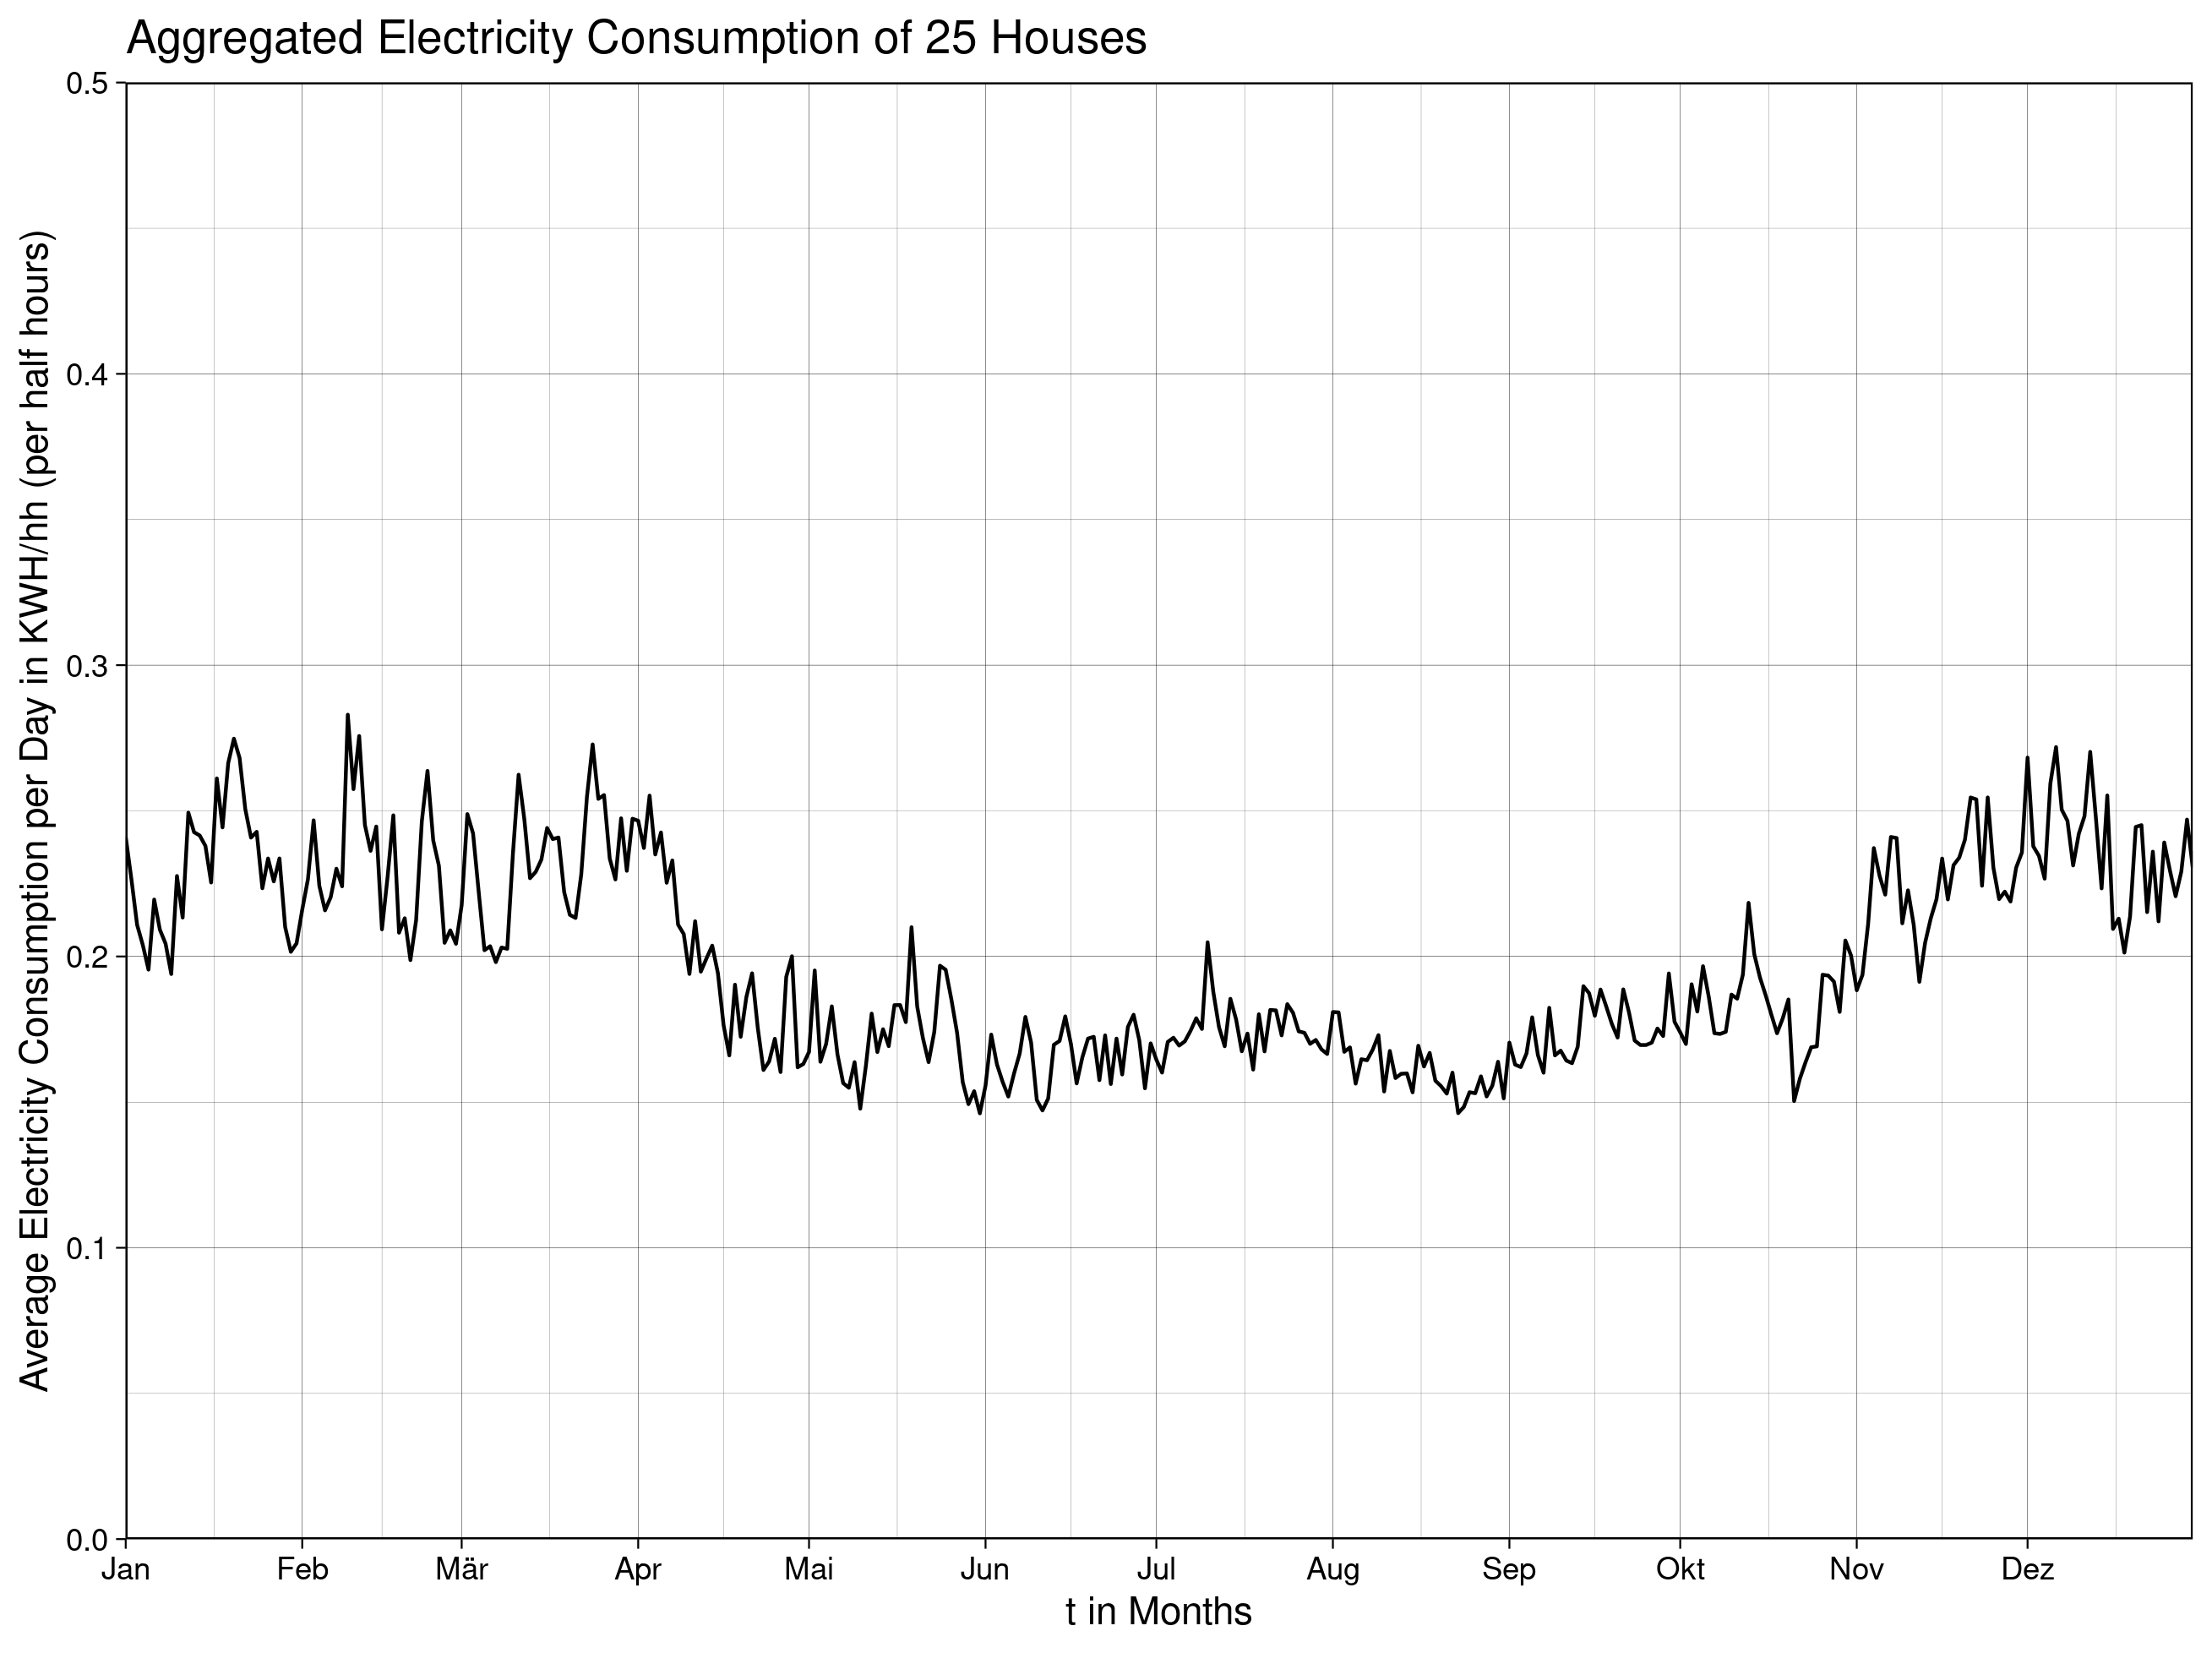
\includegraphics[width=0.85\textwidth]{images/Aggregated Electricity Consumption of 25 Houses.png}
\caption[Bandbreite Diagramm mit aktivierter Verschlüsselung]{}
\label{img:bytes-e}
\end{figure}
\begin{figure}[!p]
\centering
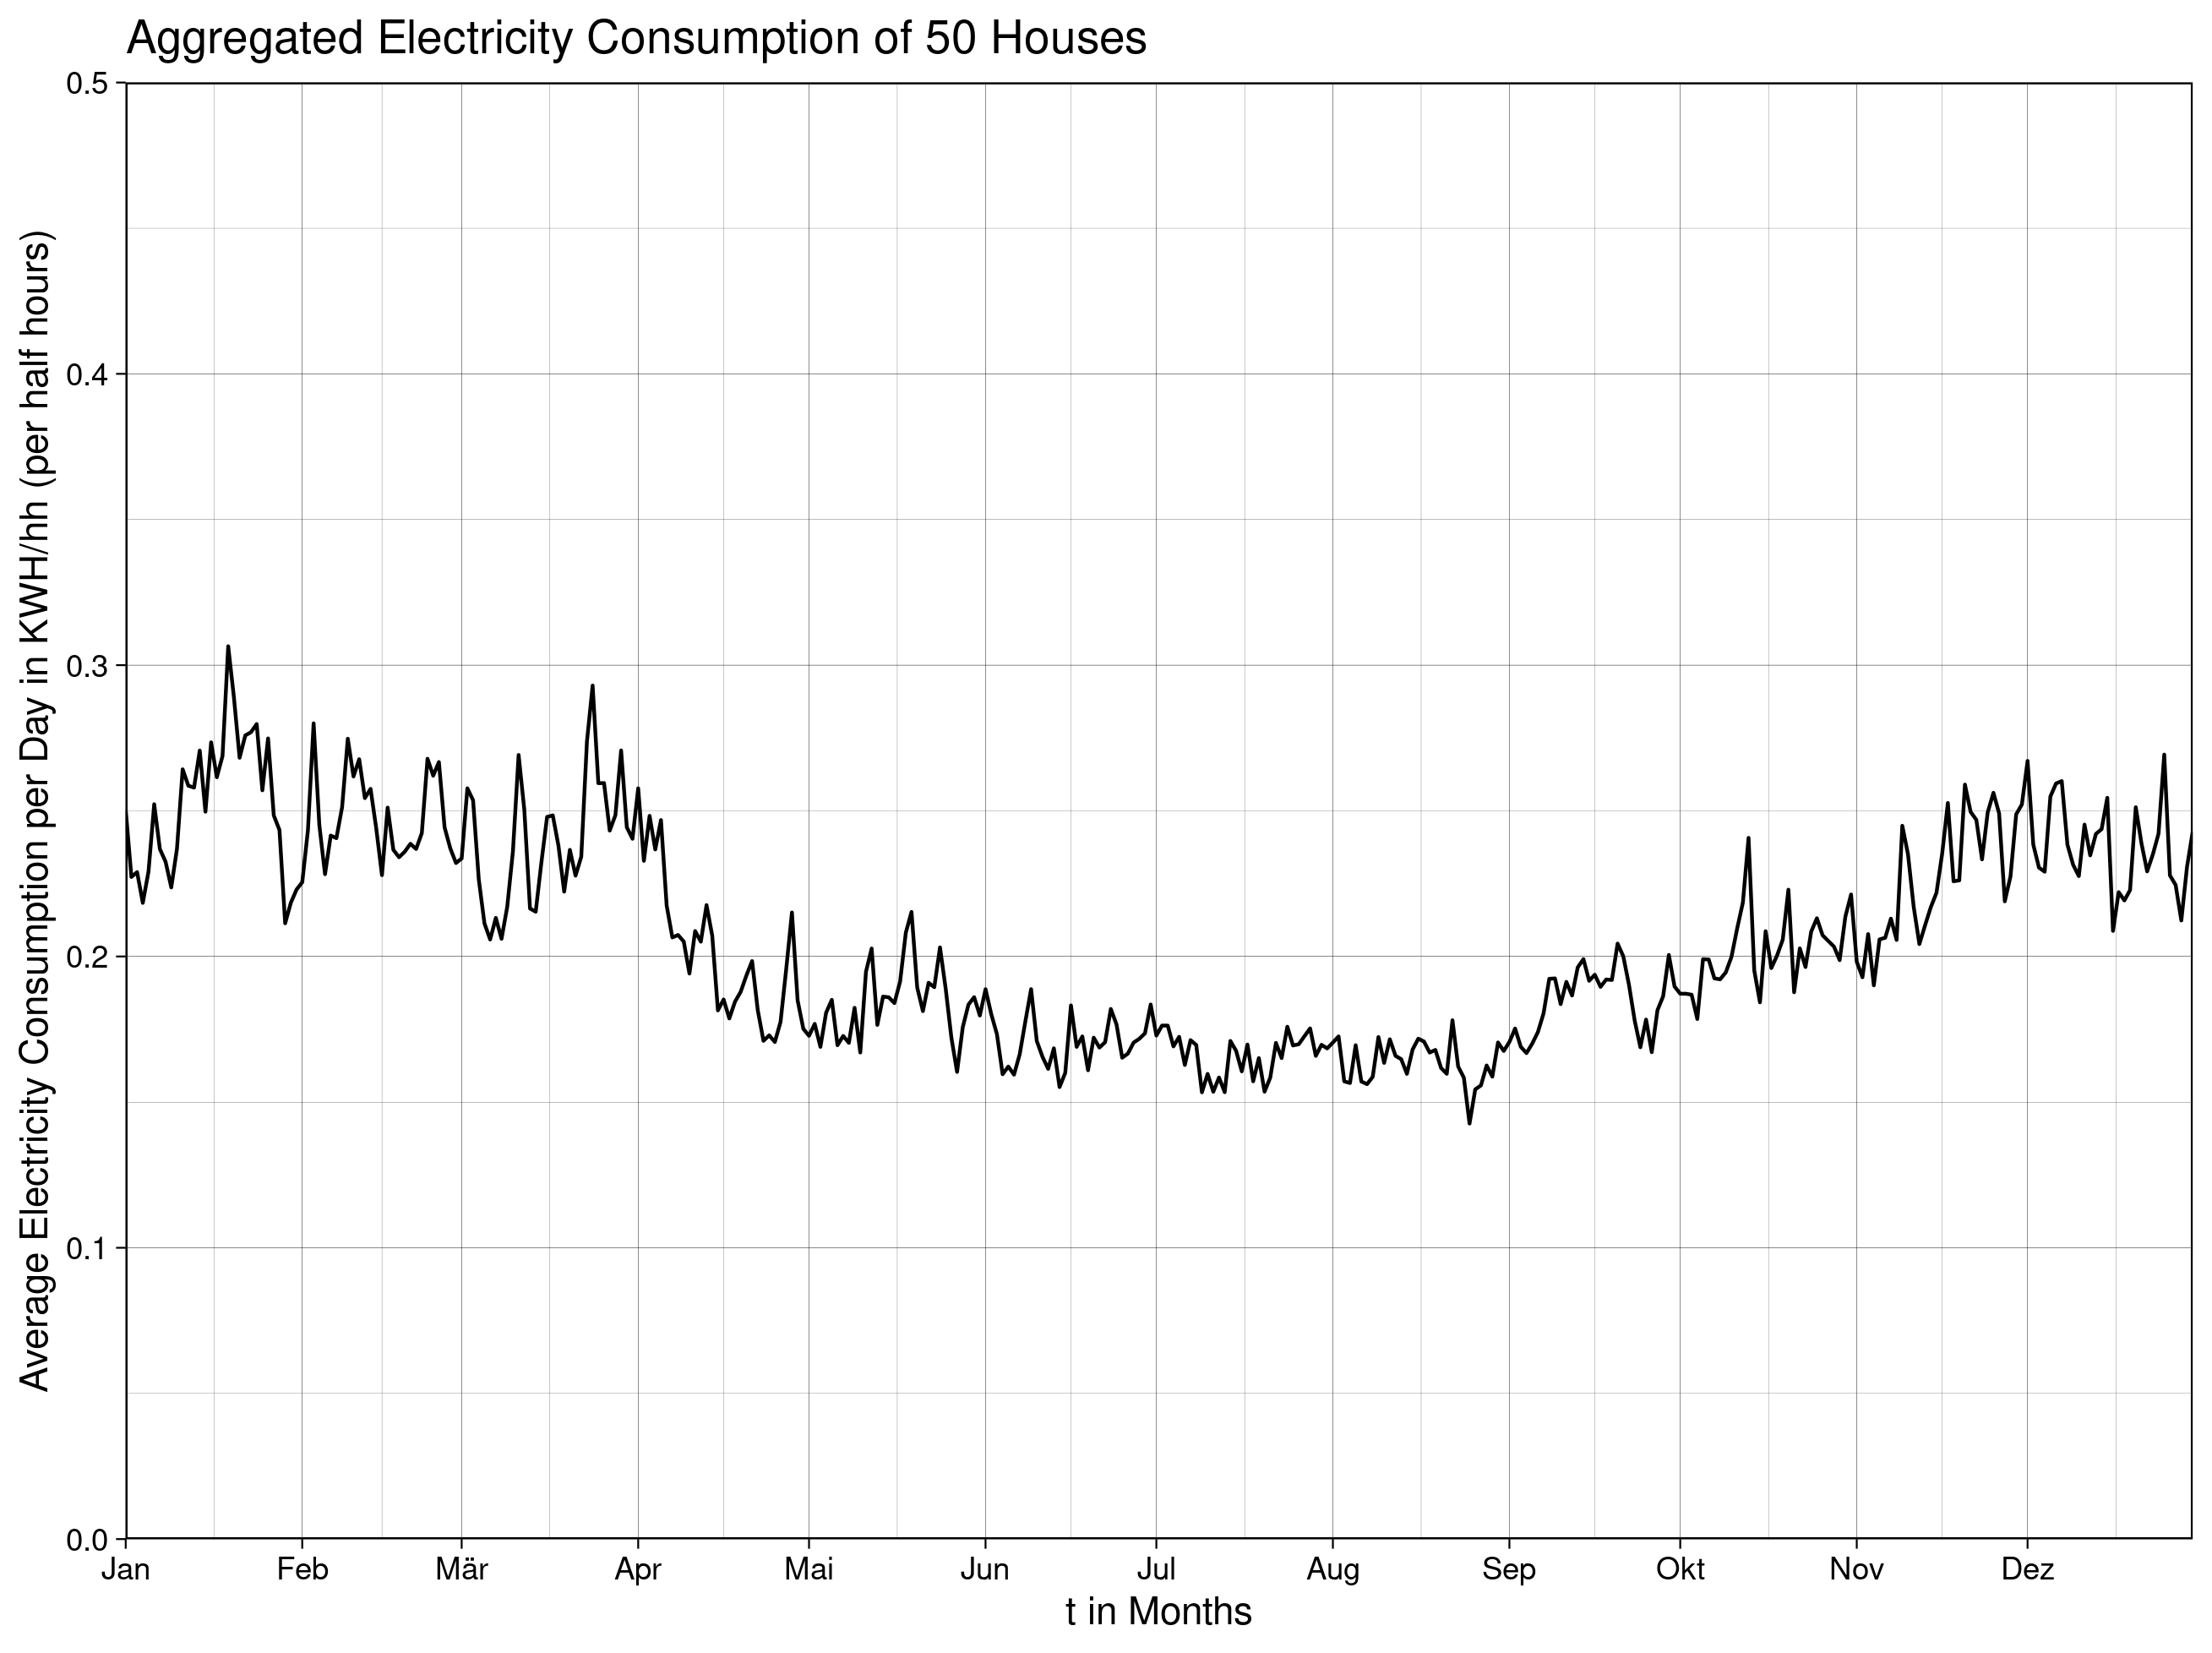
\includegraphics[width=0.85\textwidth]{images/Aggregated Electricity Consumption of 50 Houses.png}
\caption[Diagramm der Bandbreite ohne Verschlüsselung]{}
\label{img:bytes-we}
\end{figure}
\clearpage
}
\afterpage{%
\begin{figure}[!p]
\centering
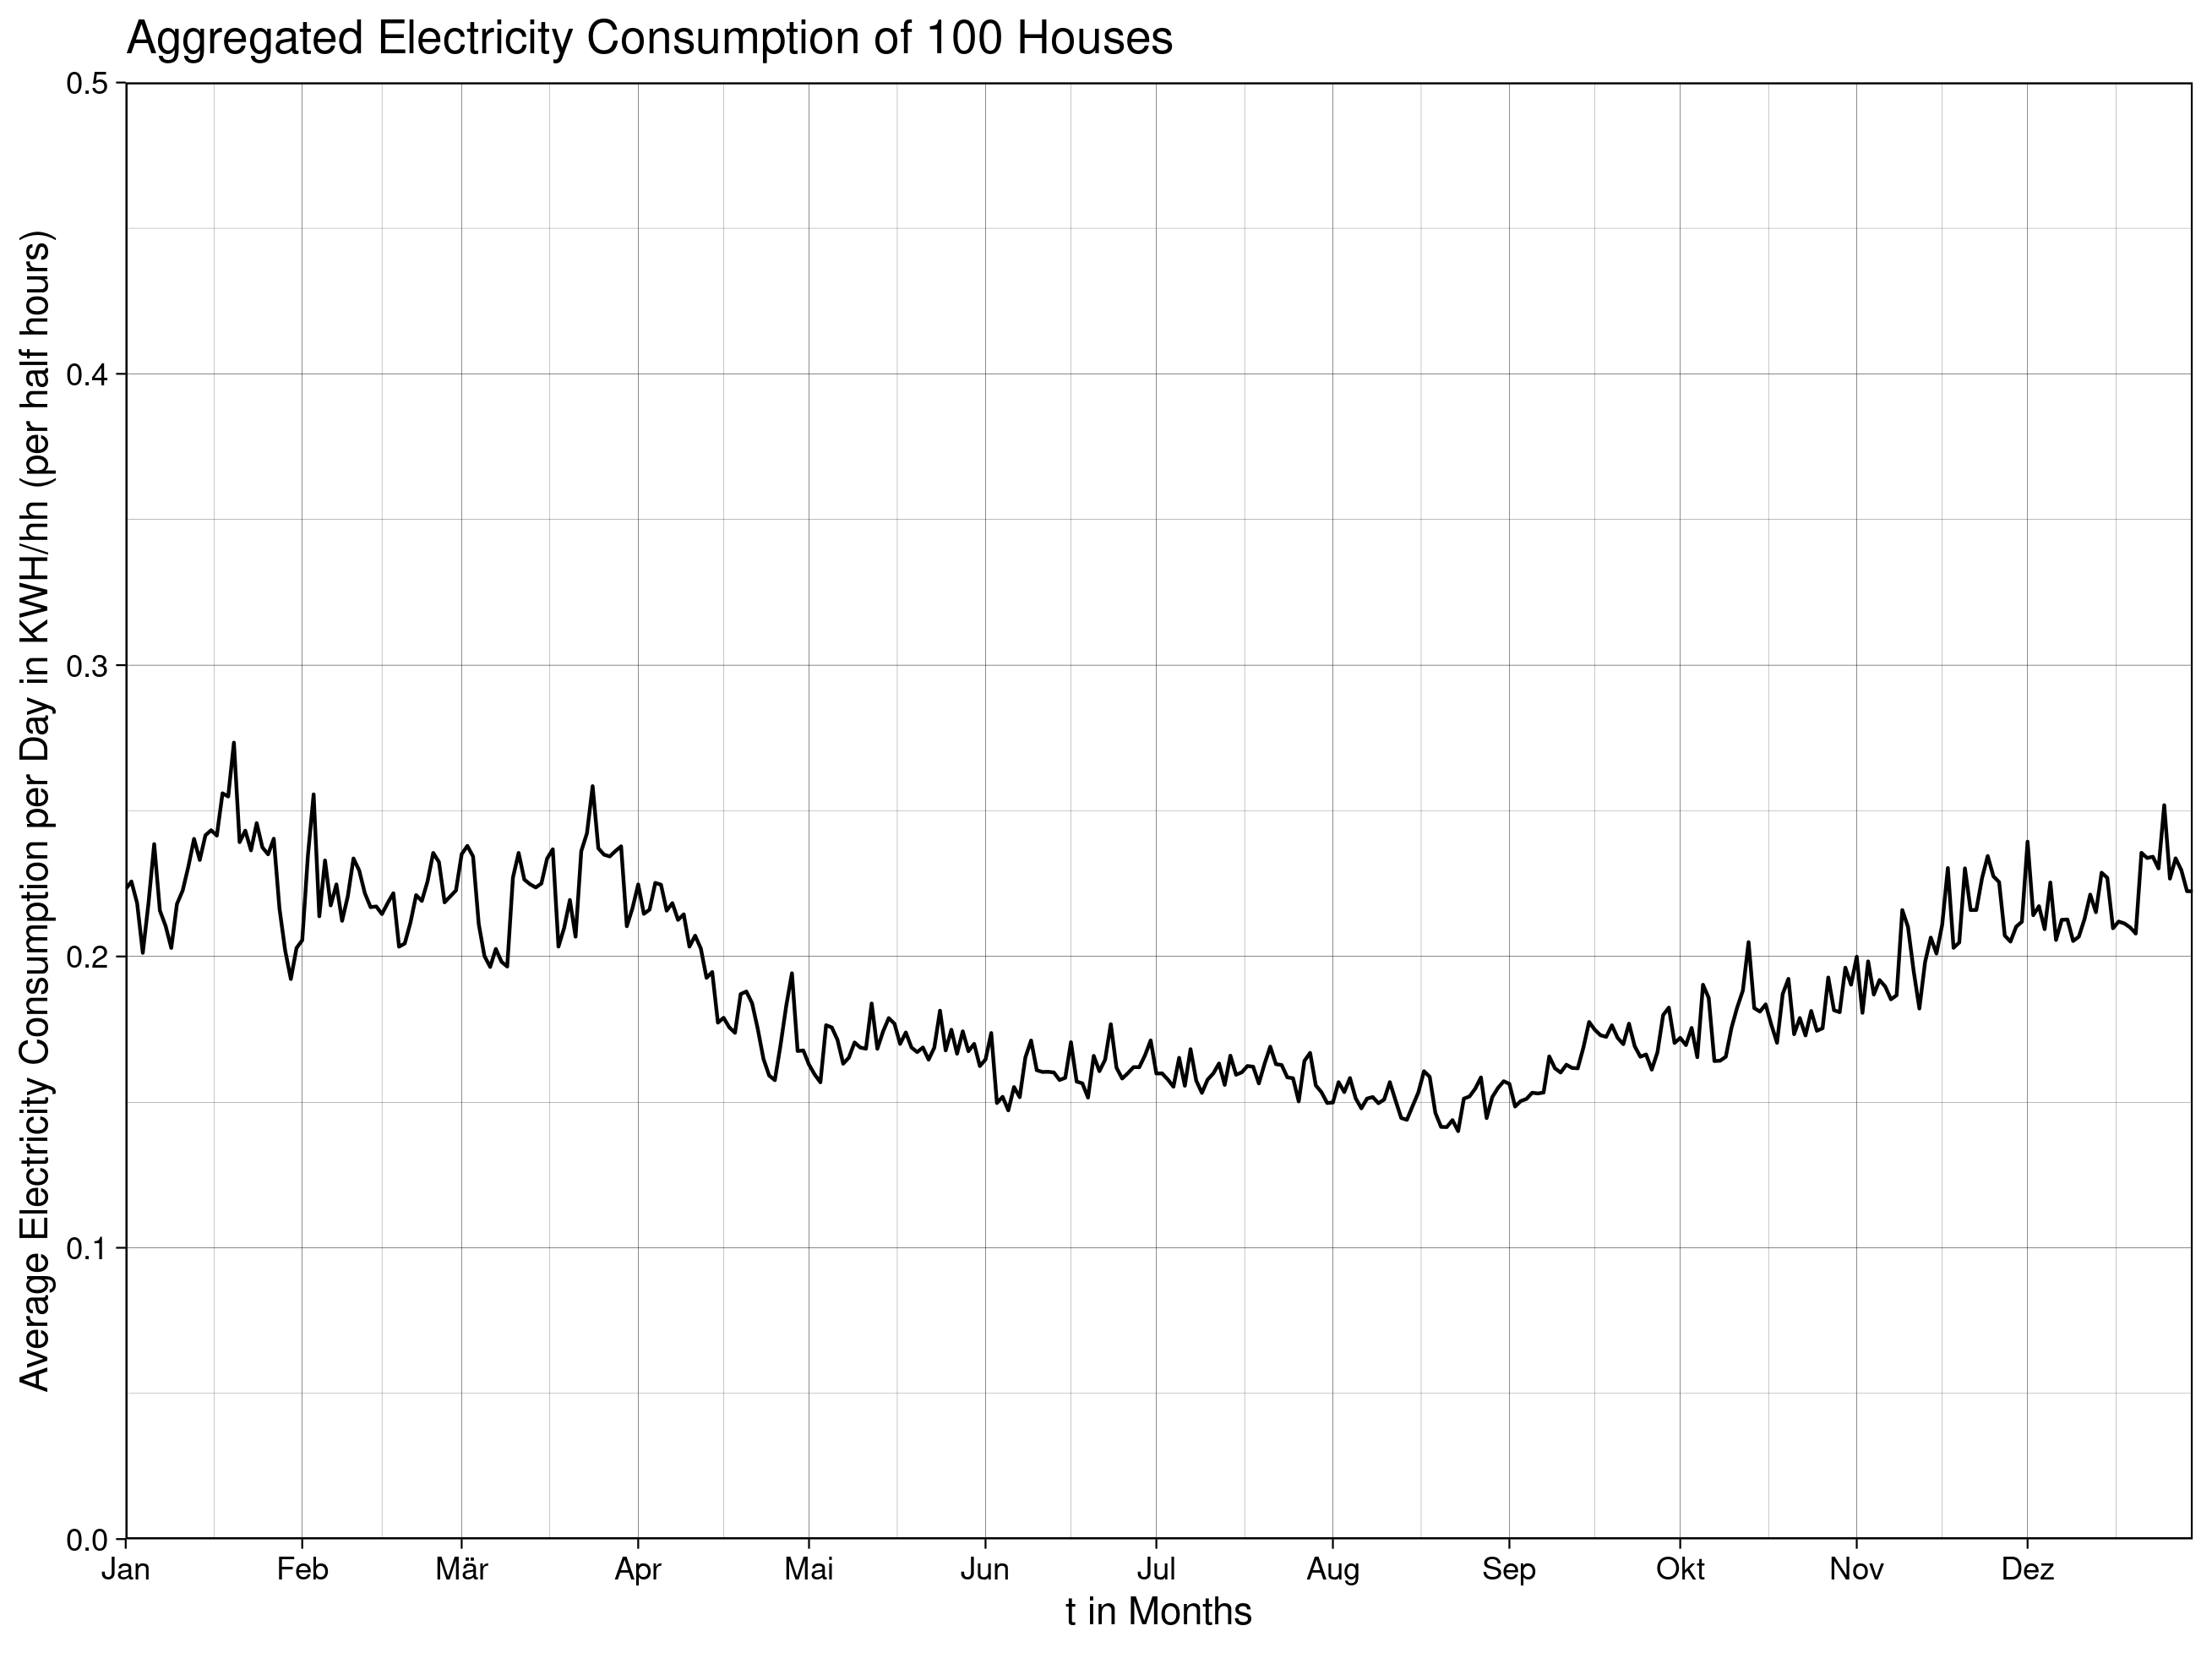
\includegraphics[width=0.85\textwidth]{images/Aggregated Electricity Consumption of 100 Houses.png}
\caption[Bandbreite Diagramm mit aktivierter Verschlüsselung]{}
\label{img:bytes-e}
\end{figure}
\begin{figure}[!p]
\centering
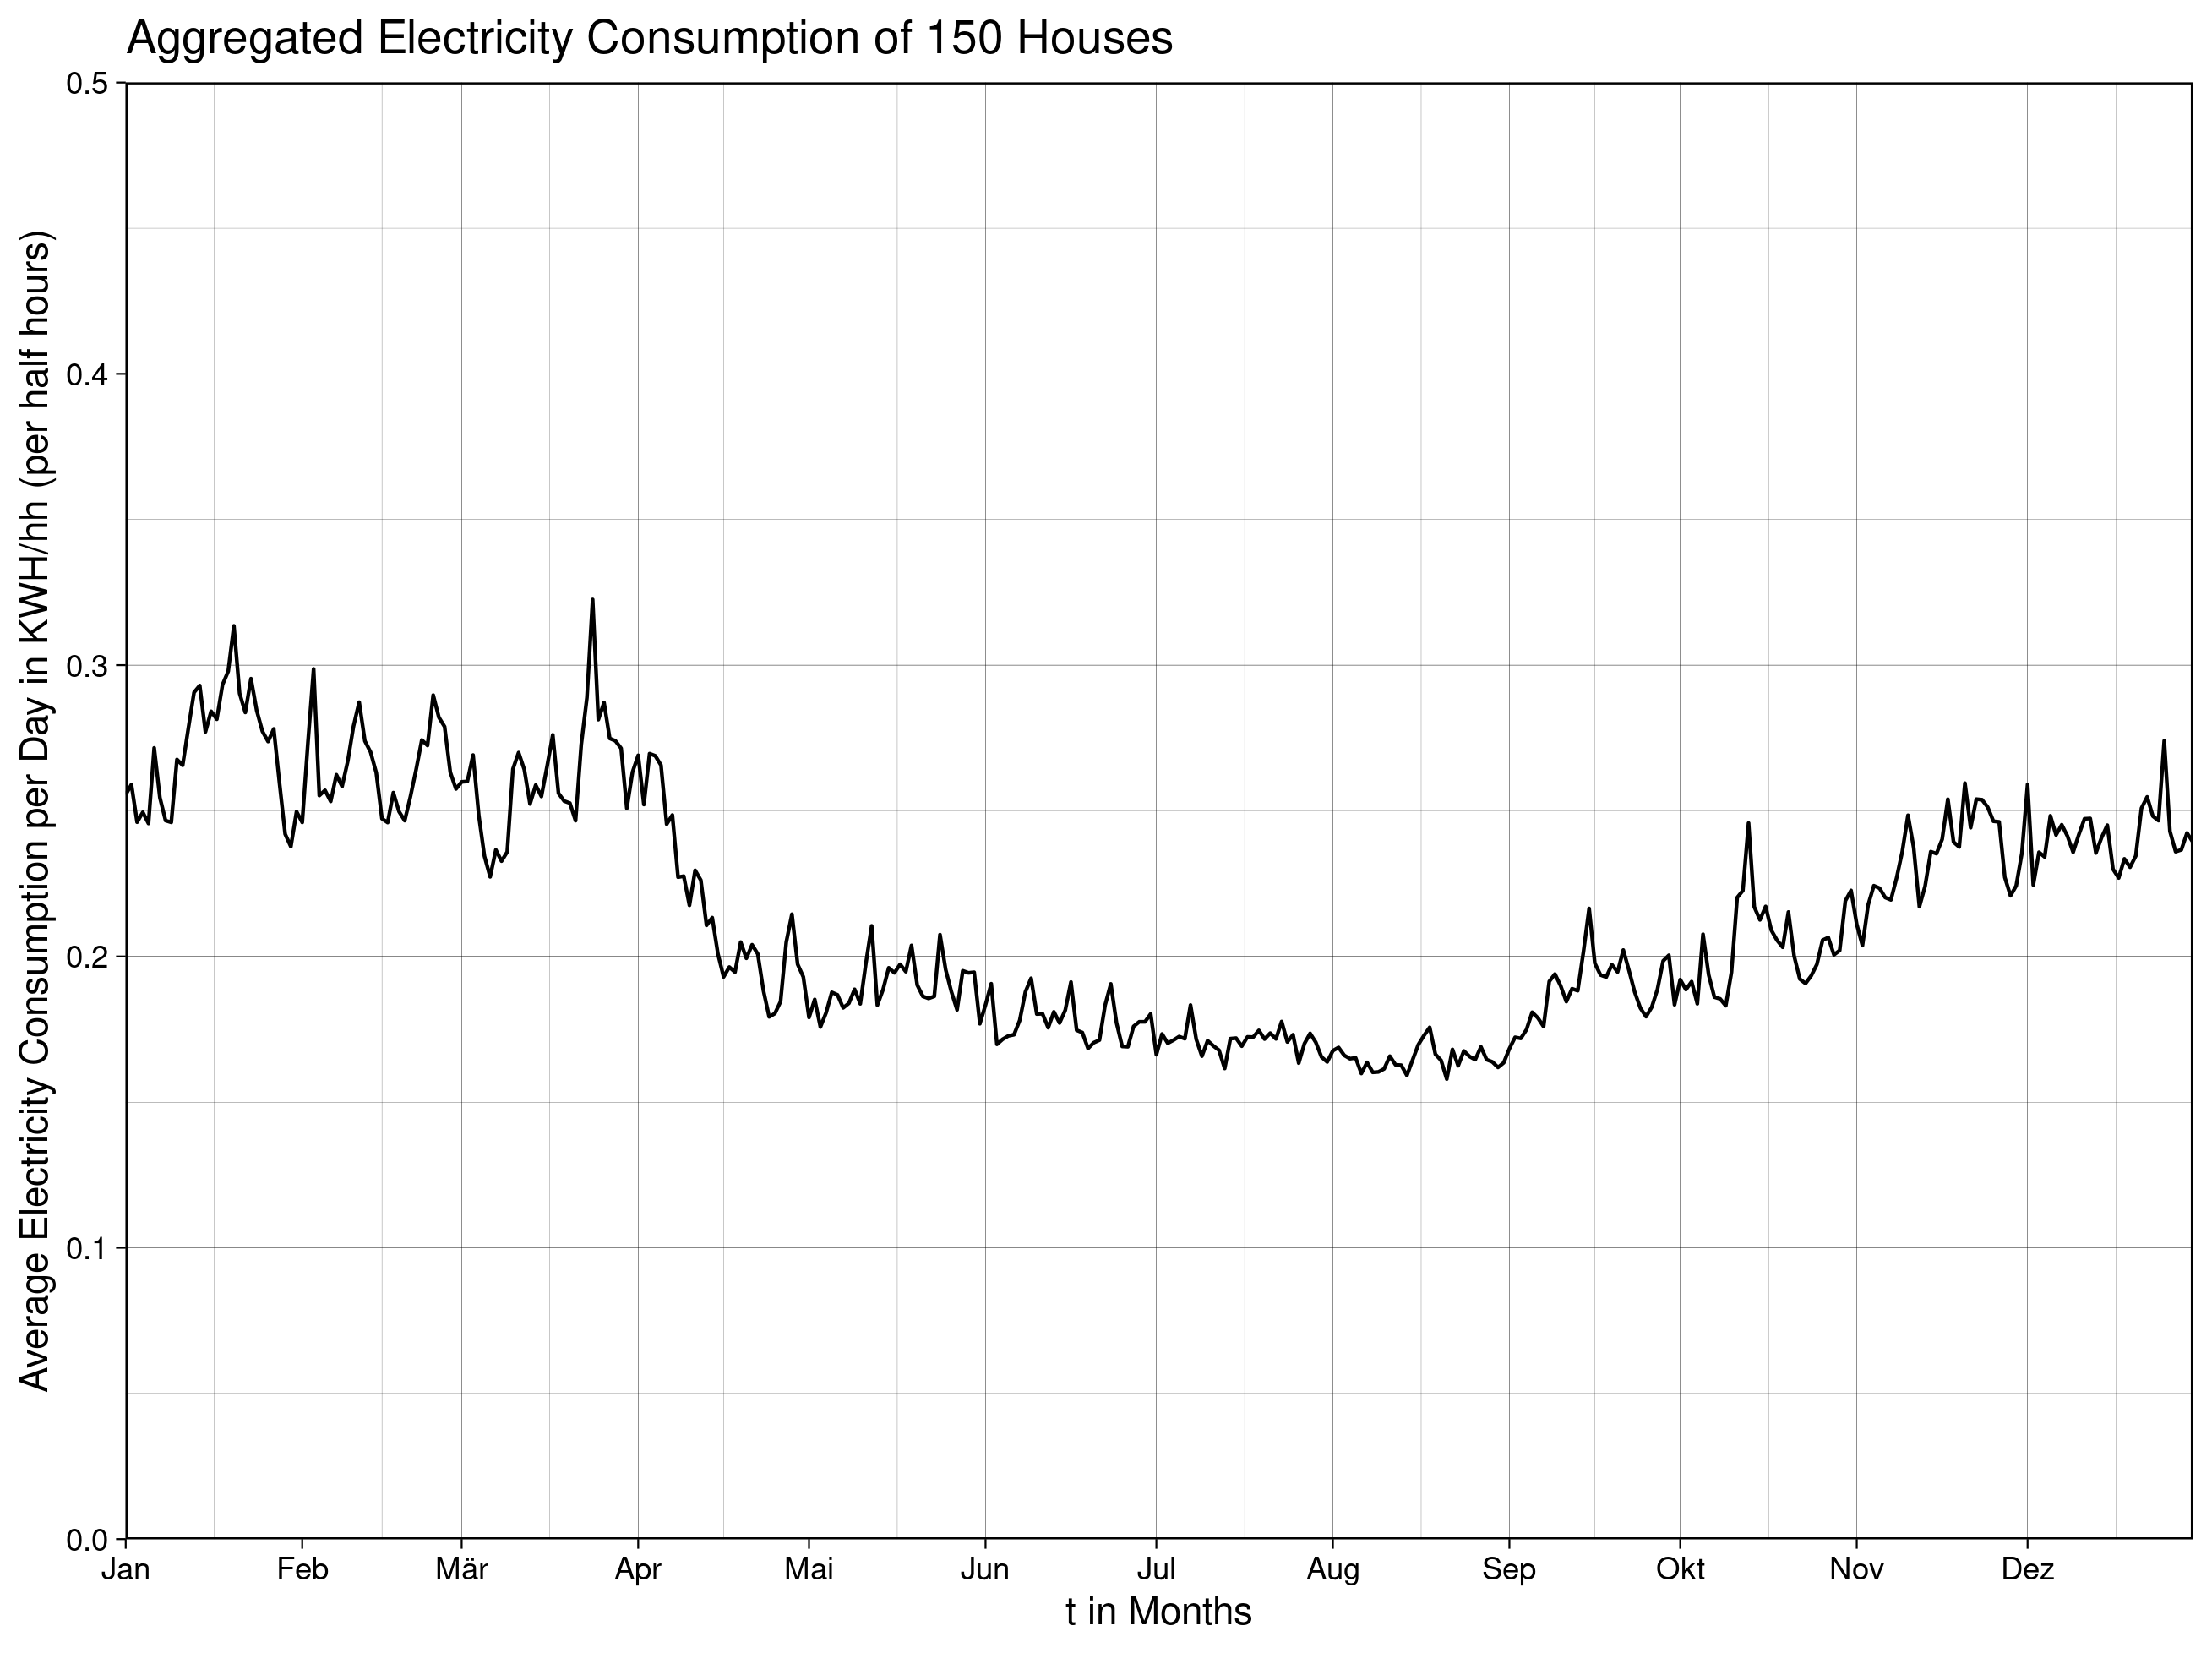
\includegraphics[width=0.85\textwidth]{images/Aggregated Electricity Consumption of 150 Houses.png}
\caption[Diagramm der Bandbreite ohne Verschlüsselung]{}
\label{img:bytes-we}
\end{figure}
\clearpage
}


\todo{letztes Experiment implementieren}

\cleardoublepage

%%% Local Variables:
%%% TeX-master: "diplom"
%%% End:

\chapter{Evaluation}
\label{Evaluation}
In this chapter the properties of the DC network are analyzed. Various characteristics are evaluated, including the performance of the process, the security and the necessary minimum size of the network.
\section{Performance}
Regarding the performance, it is considered to what extent the proposed network is more efficient or inefficient compared to the Technical Guideline.\todo{ein wenig mehr schreiben}
\\
\\
\textbf{Computational Performance}
\\
\\
The proposed DC network is highly scalable. Due to the fact that on the SGMW side only a simple computation of the power consumption with a generated key through a PRNG has to be performed to form the local sum, hardly any computational power will have to be used. Furthermore, a local sum is sent only every 15 minutes. The computational overhead caused by the sending the local sum is negligible for the SMGW and the protocol should be able to run without problems even on lightweight systems. It has to be considered that the used PRNG really generates random numbers. The built-in hardware security module in the SGMW should perform this task without faults. On the side of the power provider, only simple operations need to be performed as well. Every single local sum of a SMGW has to be added up to form the global sum. Addition of many thousands of summands is no problem for ordinary computers and the complexity of the calculation does not deviate from the proposal of the technical guideline, since the transmitted data has to be summed up as well.\\
\\
\textbf{Performance of the Error Correction}
\\
\\
The transmission bit allows the power provider to immediately detect which SMGW in the network has failed. Even if several SMGW fail at the same time, it is no issue for the neighboring SMGW to resend the updated local sum to the power provider. Then the power provider efficiently calculates the global sum [REF procedure]. \\
\\
\textbf{Message Overhead}
\\
\\
The messages sent in the protocol can be implemented with a small header. The message field in which the local sums are entered must always be the same size, otherwise the DC network cannot be implemented. Therefore, large data packets are not to be expected, since the local sums require a sufficiently large message field, which will not require more than several 100 bytes. \\
\\
\textbf{Memory Overhead}
\\
\\
The memory overhead of SMGW in a DC network is minimal. Only the PRNG key from the neighbors need to be stored. However, the power provider needs to store the key graph and the power provider has a larger storage overhead compared to the technical guideline. 
\\
\\
\textbf{Message Overhead}
\\
\\
When registering a requesting SMGW in a DC network, several messages must be exchanged between the SMGW and the electricity provider as well as between the requesting SMGW and the neighbor SMGW. If a DC network round runs without errors, no additional messages are exchanged.
In case of error correction measures, a large number of multiple messages must be sent, otherwise no meaningful global sum can be calculated and the members in a DC network must coordinate to correct the error. Considering that normally only one message is sent to the power provider every 15 minutes, it should be bearable for the power provider if there is a minimal to medium traffic volume every 15 minutes in a DC network.
\section{Security}
The security evaluation considers the extent to which the security objectives are better or worse protected compared to the technical guideline from the BSI. Possible attacks on the security objectives have already been explained in the Design chapter.
\\
\\
\textbf{Availability}
\\
\\
Availability is one of the most important security objectives of the DC network. If an SGMW should fail, e.g. due to a missing Internet connection, then no global sum can be formed and the functionality of the network is not possible. This is equivalent to an unavailable network for the power provider. Measures have been described to deal with this failure. If an attacker succeeds in taking over an SMGW, he can deliberately send incorrect local sums with the intention of disrupting availability. Against this active attack, an algorithm was proposed that allows the power provider to switch to F-mode and search for the attacker and restore availability. According to this, temporary outages may occur in the DC network, but all of them can be solved in a short time by troubleshooting procedures. A degradation of availability is therefore not expected.
\todo{Vertraulichkeit}
\\
\\
\textbf{Anonymity}
\\
\\
By using PRNG, anonymity decreases from information-theoretically secure to complexity-theoretically secure anonymity. Nevertheless even if an SMGW is controlled by an attacker, it would not be possible for the attacker to read the power consumption of other SMGWs. This is because the attacker has no access to the global total. This can only be calculated by the electricity provider. With the proposed method, the attacker lacks the necessary information to launch a potential attack on the DC network (if the attacker only has control over one SMGW). Furthermore, the attacker also has no information about the key graph. This further complicates the chances of a successful attack to deanonymize the electricity consumption of costumers. The electricity provider is potentially the most dangerous attacker in the protocol, since the SMGWs cannot communicate with each other, they rely on the electricity provider to register in the DC network. As a result, the power provider has to take over administrative tasks and therefore possesses a lot of control. To ensure that the electricity supplier is not too powerful, its competences have been restricted. The best chance of the electricity provider to break the anonymity to its customers is that the administrative powers are abused to connect individual SMGWs to malicious neighbors. Once the electricity provider manages to link an SMGW with only malicious neighbors, the local sum can be reconstructed and the electricity consumption is visible. This is prevented by forcing the electricity provider to select a random neighbor upon entry and not being able to remove SMGWs from the network on its own. These measures make it almost impossible for the electricity provider to affect the selection of neighbors in the DC network.
\\
\\
\textbf{Eavesdropping}
\\
\\
In the case of eavesdropping on one or more lines of SMGWs by an attacker, attackers can read but not understand payload data because the local sum is not a meaningful message. An attacker can therefore only observe when an SMGW sends local sums. Furthermore, the attacker can assume from an increased message volume that an error correction procedure is being used in the DC network. 
\\
\\
\textbf{Malicious Electricity Provider}
\\
\\
The strongest attacker in the DC network is an electricity provider that has malicious intent with the motivation to obtain additional privacy compromising data. Due to the advanced administrative functions available to the electricity provider, the electricity provider could be tricked into exploiting its administrative rights. Therefore, there is a fine line between granting administrative privileges to the electricity provider to maintain the DC network and restricting administrative privileges so that the electricity provider cannot breach security. Careful consideration has been given in the design to what powers are necessary for the electricity provider. However, if a malicious power provider does tamper with the DC network, the SGMW will have the ability to leave the DC network.
\\
\\
\textbf{Protocol compatibility with the TR}
\\
\\
The protocol has been designed with the structural specifications of the technical guideline. Therefore, after implementation, it could be integrated into the currently specified German smart grid without any major complications. The WAN interface of the SMGW does not need to be extended and existing communication links are not affected by the protocol. 


\todo{vllt noch ein wenig mehr?}

\clearpage

%%% Local Variables:
%%% TeX-master: "diplom"
%%% End:

\chapter{Conclusion and Future Work}
\label{sec:conclusion}

%  Schlußfolgerungen, Fragen, Ausblicke

% Dieses Kapitel ist sicherlich das am Schwierigsten zu schreibende. Es
% dient einer gerafften Zusammenfassung dessen, was man gelernt hat. Es
% ist möglicherweise gespickt von Rückwärtsverweisen in den Text, um dem
% faulen aber interessierten Leser (der Regelfall) doch noch einmal die
% Chance zu geben, sich etwas fundierter weiterzubilden. Manche guten
% Arbeiten werfen mehr Probleme auf als sie lösen. Dies darf man ruhig
% zugeben und diskutieren. Man kann gegebenenfalls auch schreiben, was
% man in dieser Sache noch zu tun gedenkt oder den Nachfolgern ein paar
% Tips geben. Aber man sollte nicht um jeden Preis Fragen, die gar nicht
% da sind, mit Gewalt aufbringen und dem Leser suggerieren, wie
% weitsichtig man doch ist. Dieses Kapitel muß kurz sein, damit es
% gelesen wird.
Smart meters offer a great opportunity to automate the existing power grid and increase the quality in the grid \ref{sec:intro}. At the same time, smart meters can be misused to create accurate behavior profiles of individuals in their own homes \ref{subsec:NILM_sec}. The \gls{BSI}'s \gls{TR-03109} is a first standard that establishes uniform requirements for the security of smart meters and provides a minimum level of protection. Nevertheless, analyses of electricity consumption can be carried out by the electricity provider without any major effort, as pseudonymization alone cannot prevent this \ref{sec:TR_03109}. Therefore, a technical solution to the problem must be found and a variety of proposals are already being considered in the scientific community.\\ This work deals with DC networks, which are classified as aggregation without trusted third party methods. DC networks have not been considered in detail in science as a solution for privacy-preserving smart grids. The proposed design is a dc network based network protocol, which follows the requirements of the \gls{BSI} \gls{TR-03109}. Even though not all requirements of the \gls{TR-03109} could be implemented in detail, the considered design can be adopted in the German Smart Grid without major structural changes to the existing infrastructure or software \ref{sec:design}. The solution therefore deviates from the original DC network as described e.g. in \cite{chaum1988dining}, because the restrictions of the \gls{TR-03109} would not be compatible with a normal DC network and the classical DC network could not be implemented. Therefore, the electricity provider must be given administrative authority over the DC network as well as over the key graph in order for the DC network to be compliant with the \gls{BSI} \gls{TR-03109}. The proposed design changes had to be weighed throughout that, on the one hand, the DC network does not lose in security and anonymity. On the other hand, the proposed DC network must be efficient and operable in the real world with the administrative powers of the power provider. It must be able to dynamically respond to errors and fend off potential attackers. The two requirements of security and operability have always been at odds with each other and have meant that any change to the classic DC network has had to be carefully considered. \\
In the chapter \ref{Evaluation}, the characteristics of the proposed DC network were considered in terms of security and performance. While there may be an overhead in terms of message volume, the DC network does not lose in security compared to the classical DC network. In the case of an attacker, the power provider has procedures available to protect its network \ref{error_corr} and in the case of the strongest attacker, namely a malicious power provider, the clients have options available to protect themselves from the power provider. Furthermore, the design of the network provides many hurdles for the DC network to be structurally protected from a malicious power provider. The increased message volume is negligible since the power consumption is sent only every 15 minutes and likewise error correction actions result in only a slightly higher message volume. Moreover, the proposed DC network is scalable and can handle large numbers of users~\ref{performance}.\\
In addition, the proposed DC network was implemented on four Raspberry Pis (three clients and one electricity provider) to simulate real conditions and prove that it is a workable and viable protocol. Furthermore, a stochastic experiment was implemented to study how the information content of electricity consumption is preserved in aggregated results, so that also no conclusions can be drawn from the aggregated result. The findings from the experiments were used to obtain a minimum number of DC network participants. The results show that a high level of anonymity can be achieved with as few as 10 - 25 participants (see \ref{sec:experiments}). \\
\\
\textbf{Future Work}
\\
\\
In the case of the manipulation of the local superposition \ref{subsec:mani_local}, the algorithm could not be implemented in the demo. Since the algorithm was defined by the author and not implemented, the correctness of the algorithm cannot be answered with complete certainty. \\
Furthermore, the experiments looked for a minimum number of participants in a DC network. Different metrics were used and the results were analyzed. To get further clarity on the minimum number of DC networks, it would be possible to perform a cluster analysis and linear regression. 


%\todo{der algo wurde nicht auf korrektheit überprüft? wo das hinschreiben in Conclusion oder in evaluation?}

\cleardoublepage

%%% Local Variables:
%%% TeX-master: "diplom"
%%% End:


\appendix

%\addchap{Glossar}

% makeglossaries diplom
%\printglossary[style=altlist]
%\printglossary[type=\acronymtype,style=long]

\printbibliography
\iffalse
    % an aid for Kile autocompletion
    \bibliography{own.bib}
\fi

\end{document}
